\documentclass{article}

\usepackage[utf8]{inputenc}
\usepackage{graphicx}
\usepackage{amsmath}
\usepackage{amsfonts}
\usepackage{textcomp}
\usepackage{amssymb}
\usepackage{amsthm}
\usepackage{subcaption}
\usepackage{times}
\usepackage[portuguese]{babel}
\usepackage{geometry}
\geometry{a4paper, left=3cm, top=3cm, right=2cm, bottom=2cm}
\usepackage{multicol}

\title{\textbf{Cálculo 1}}
\author{Notas de aulas de Luiz Antônio, escrito por Caio Tomás. Curso ministrado no ano de 2018.\\ Ref.: Um curso de Cálculo vol.1, Guidorizzi}
\date{}
\begin{document}
{\fontfamily{ptm}\selectfont
\begin{titlepage}
\clearpage \maketitle \thispagestyle{empty}
\end{titlepage}

\clearpage \tableofcontents \thispagestyle{empty}

\begin{newpage}
\section{Limites}
\subsection{Limite e continuidade- uma noção intuitiva}
\hspace{12pt} Intuitivamente, dizer que uma função $f$ é contínua em um ponto $p$ de seu domínio quer dizer que $f$ não apresenta ''salto'' em $p$. Podemos dizer também que, se é possível desenhar o gráfico de $f$ sem retirar o lápis do papel, então $f$ é contínua em todo seu domínio.
\par Também intuitivamente, dizer que o limite de $f(x)$, quando $x$ tende a $p$, é igual a $L$, significa que quando $x$ se aproxima de $p$, $f(x)$ se aproxima de $L$. Em símbolos, escrevemos:
\begin{equation*}\displaystyle{\lim_{x\to p}f(x) = L}.\end{equation*}
\par Por fim, também intuitivamente, é razoável esperar que se $f$ estiver definida em $p$ e for contínua em $p$, então $\displaystyle{\lim_{x\to p}f(x) = f(p)}$, e reciprocamente. É possível provar que isso realmente é verdade, isto é, $f$ é contínua em $p$ se, e somente se $\displaystyle{\lim_{x\to p}f(x) = f(p)}$. A título de curiosidade, tanto a definição formal quanto a demonstração dessa relação são tratados em cursos de análise real. Aqui as definições formais serão apresentadas, somente para proporcionar um primeiro contato com a análise.
\par
\vspace{0.3cm}  
\subsection{Exercícios iniciais - limite}
\begin{flushleft}
1. Calcule os limites abaixo.
\end{flushleft}
\begin{multicols}{3}
a)$\displaystyle{\lim_{x\to\ -3} \frac{x^2 - 9}{x+3}}$\\
b)$\displaystyle{\lim_{x\to\ -\frac{3}{2}} \frac{6x^2 + 11x + 3}{2x^2 - 5x - 12}}$\\
c)$\displaystyle{\lim_{x\to\ -1} \frac{x^3 + 3x^2 -x - 3}{x^3 - x^2 + 2}}$
\end{multicols}
\par
\begin{flushleft}
1.1 Resolução.
\end{flushleft}
\vspace{0.3cm}
\par
a)$\displaystyle{\lim_{x\to-3} \frac{x^2 - 9}{x+3} =
\lim_{x\to-3} \frac{(x+3)(x-3)}{(x+3)} =
\lim_{x\to-3} (x-3) = -6}$.
\vspace{0.3cm}
\par
b)$\displaystyle{\lim_{x\to -\frac{3}{2}} \frac{6x^2 + 11x + 3}{2x^2 - 5x - 12} = \lim_{x\to -\frac{3}{2}} \frac{(x+3/2)(6x+2)}{(x+3/2)(2x-8)} = \lim_{x\to -\frac{3}{2}} \frac{3x + 1}{x-4} = \frac{7}{11}}$.
\vspace{0.3cm}
\par
c)$\displaystyle{\lim_{x\to -1} \frac{x^3 + 3x^2 -x - 3}{x^3 - x^2 + 2} = \lim_{x\to -1} \frac{(x+1)(x^2 + 2x - 3)}{(x+1)(x^2 - 2x + 2)} = -\frac{4}{5}}$.
\vspace{0.3cm}
\begin{flushleft}
2. Calcule $\displaystyle{\lim_{h\to 0} \frac{f(x+h) - f(x)}{h}}$, sendo $f$ dado por:
\end{flushleft}
\par
\begin{multicols}{3}
\hspace{-15pt}a)$f(x)=x^2$\\
b)$f(x)=2x^2 + x$\\
c)$f(x)=5$\\
d)$f(x)=-x^3 + 2x$\\
e)$f(x)=1/x$\\
f)$f(x)=3x+1$
\end{multicols}
\vspace{0.3cm}
\begin{flushleft}
2.1 Resolução.
\end{flushleft}
\par
\vspace{0.3cm}
a)$\displaystyle{\lim_{h\to 0} \frac{(x+h)^2 - x^2}{h} = \lim_{h\to\ 0} \frac{2xh + h^2}{h} = 2x}$.
\par
\vspace{0.3cm}
b)$\displaystyle{\lim_{h\to 0} \frac{2(x+h)^2 + (x+h) - 2x^2 - x}{h} = \lim_{h\to\ 0} \frac{4xh + 2h^2 + h}{h} = 4x + 1}$.
\par
\vspace{0.3cm}
c)$\displaystyle{\lim_{h\to 0} \frac{5-5}{h} = \lim_{h\to\ 0} 0 = 0}$.
\par
\vspace{0.3cm}
d)$\displaystyle{\lim_{h\to 0} \frac{-(x+h)^3 + 2(x+h) + x^3 - 2x}{h} =\lim_{h\to\ 0} \frac{-3hx^2 - 3xh^2 - h^3 + 2h}{h} = -3x^2 + 2}$.
\par
\vspace{0.3cm}
e)$\displaystyle{\lim_{h\to 0} \frac{\frac{1}{x+h} - \frac{1}{x}}{h} =\lim_{h\to 0} \frac{-h}{x(x+h)h} = -\frac{1}{x^2}}$.
\par
\vspace{0.3cm}
f)$\displaystyle{\lim_{h\to 0} \frac{3(x+h) + 1 - 3x - 1}{h} = \lim_{h\to 0} \frac{3h}{h}= 3}$.
\par
\vspace{0.3cm}
\textbf{Observação}: Nas resoluções anterirores foi possível simplificar expressões do tipo $x/x$ porque dizer que $x$ \textit{tende} a zero é diferente de dizer que $x$ \textit{é} zero. Dizer que $x$ tende a zero é dizer que $x$ está tão próximo de zero quanto quisermos sem, contudo, assumir o valor zero. Essa formulação pode parecer um pouco esquisita, mas em análise real provamos esse fato rigorosamente, utilizando $\epsilon $ (épsilon) e $\delta $ (delta). A definição formal de limite será apresentada mais à frente, com o simples objetivo de lhe dar uma amostra da análise real. Após eliminada a indeterminação (se houver) podemos admitir que $x$ é zero para o cálculo do limite.
\subsection{Propriedades operatórias}
\textbf{Teoremas.}
\par
\vspace{0.3cm}
Se $\displaystyle{\lim_{x\to a} f(x) = L}$ e $\displaystyle{\lim_{x\to a} g(x) = M}$, então:
\par
\vspace{0.2cm}
1.$\displaystyle{\lim_{x\to a} (f(x) + g(x)) = \lim_{x\to a} f(x) + \lim_{x\to a} g(x) = L + M}$;
\par
\vspace{0.2cm}
2.$\displaystyle{\lim_{x\to a} (f(x) - g(x)) = \lim_{x\to a} f(x) - \lim_{x\to a} g(x) = L - M}$;
\par
\vspace{0.2cm}
3.$\displaystyle{\lim_{x\to a} (f(x)g(x)) = (\lim_{x\to a} f(x))(\lim_{x\to a} g(x)) = L\cdot M}$;
\par
\vspace{0.2cm}
4.$\displaystyle{\lim_{x\to a} \frac{f(x)}{g(x)} = \frac{\lim_{x\to a} f(x)}{\lim_{x\to a} g(x)} = \frac{L}{M}, M\neq 0}$;
\par
\vspace{0.2cm}
5.$\displaystyle{\lim_{x\to a} (f(x))^n = (\lim_{x\to a} f(x))^n = L^n, \forall n\in\mathbb{N}}$;
\par
\vspace{0.2cm}
6.$\displaystyle{\lim_{x\to a} \sqrt[n]{f(x)} = \sqrt[n]{\lim_{x\to a} f(x)} = \sqrt[n]{L}}$, com $L\geq 0$ se $n$ for par natural não nulo e $L\in\mathbb{R}$ se $n$ for natural ímpar.
\vspace{0.2cm}
\par
\begin{flushleft}
3. Calcule:
\end{flushleft}
\begin{multicols}{3}
\hspace{-15pt}a) $\displaystyle{\lim_{x\to 2} \frac{x^2 - 4}{\sqrt{x+2} - \sqrt{3x-2}}}$\\
b) $\displaystyle{\lim_{x\to 2} \frac{\sqrt{3x - 2} - 2}{\sqrt{4x + 1} - 3}}$\\
c) $\displaystyle{\lim_{x\to 1} \frac{x^n - 1}{x - 1}}$, $n\in\mathbb{N^*}$   \\
d) $\displaystyle{\lim_{x\to 2} \frac{\sqrt[3]{5x - 2} - 2}{\sqrt{x - 1} - 1}}$\\
e) $\displaystyle{\lim_{x\to 0} \frac{\sqrt{x+1} - 1}{\sqrt[3]{x+1} - 1}}$
    \\
f) $\displaystyle{\lim_{x\to 1} \frac{\sqrt[3]{x} - 1}{\sqrt[4]{x} - 1}}$
\end{multicols}
\par
\vspace{0.3cm}
\begin{flushleft}
4. Seja $f$ definida em $\mathbb{R}$. Suponha que $\displaystyle{\lim_{x\to 0} \frac{f(x)}{x} = 1}$. Calcule:
\end{flushleft}
\par
\begin{multicols}{4}
a) $\displaystyle{\lim_{x\to 0} \frac{f(3x)}{x}}$\\
b) $\displaystyle{\lim_{x\to 0} \frac{f(x^2)}{x}}$             \\
c) $\displaystyle{\lim_{x\to 1} \frac{f(x^2 - 1)}{x-1}}$       \\
d) $\displaystyle{\lim_{x\to 0} \frac{f(7x)}{3x}}$     
\end{multicols}
\par
\vspace{0.3cm}
\begin{flushleft}
5. Seja $f$ definida em $\mathbb{R}$ e $p$ um número real dado. Suponha que $\displaystyle{\lim_{x\to p} \frac{f(x) - f(p)}{x-p} = L}$. Calcule:
\end{flushleft}
\par
\begin{multicols}{4}
\hspace{-15pt}a) $\displaystyle{\lim_{h\to 0} \frac{f(p+h) - f(p)}{h}}$\\
b) $\displaystyle{\lim_{h\to 0} \frac{f(p+3h) - f(p)}{h}}$\\
c) $\displaystyle{\lim_{h\to 0} \frac{f(p-h) - f(p)}{h}}$--\\
d) $\displaystyle{\lim_{h\to 0} \frac{f(p+h) - f(p-h)}{h}}$
\end{multicols}
\par
\vspace{0.3cm}
\begin{flushleft}
3.1 Resolução.
\end{flushleft}
\par
a) $\displaystyle{\lim_{x\to 2} \frac{x^2 - 4}{\sqrt{x+2} - \sqrt{3x-2}} = \lim_{x\to 2} \frac{(x-2)(x+2)(\sqrt{x+2} + \sqrt{3x - 2})}{-2x + 4} = \lim_{x\to 2} \frac{(x+2)(\sqrt{x+2}+\sqrt{3x - 2})}{-2} = -8}$.
\par
\vspace{0.3cm}
b) $\displaystyle{\lim_{x\to 2} \frac{\sqrt{3x - 2} - 2}{\sqrt{4x + 1} - 3} = \lim_{x\to 2} \frac{(3x - 2 - 4)(\sqrt{4x + 1} + 3)}{(4x + 1 - 9)(\sqrt{3x - 2} + 2)} = \lim_{x\to 2} \frac{3(x-2)(\sqrt{4x + 1} + 3)}{4(x-2)(\sqrt{3x - 2} + 2)} = \frac{9}{8}}$.
\par
\vspace{0.3cm}
c) $\displaystyle{\lim_{x\to 1} \frac{x^n - 1}{x - 1} = \lim_{x\to 1} \frac{(x^{n-1} +  x^{n-2} + ... + x + 1)(x-1)}{x-1} = n}$.
\par
\vspace{0.3cm}
d) $\displaystyle{\lim_{x\to 2} \frac{\sqrt[3]{5x - 2} - 2}{\sqrt{x - 1} - 1} = \lim_{x\to 2} \frac{(\sqrt[3]{5x - 2} - 2)((5x-2)^{2/3} + 2(5x - 2)^{1/3} + 4)(\sqrt{x-1} + 1)}{(\sqrt{x-1} - 1)(\sqrt{x-1} + 1)((5x-2)^{2/3} + 2(5x - 2)^{1/3} + 4)}} =$ \par $= \displaystyle{\lim_{x\to 2} \frac{5(x-2)(\sqrt{x-1} + 1)}{(x-2)((5x-2)^{2/3} + 2(5x - 2)^{1/3} + 4)} = \frac{5}{6}}$.
\par
\vspace{0.3cm}
e) $\displaystyle{\lim_{x\to 0} \frac{\sqrt{x+1} - 1}{\sqrt[3]{x+1} - 1} = \lim_{x\to 0} \frac{(\sqrt{x+1} - 1)(\sqrt{x+1} + 1)((x+1)^{2/3} + (x+1)^{1/3} + 1)}{(\sqrt[3]{x+1} - 1)((x+1)^{2/3} + (x+1)^{1/3} + 1)(\sqrt{x+1} + 1)}} =$ \par  $=\displaystyle{\lim_{x\to 0} \frac{x((x+1)^{2/3} + (x+1)^{1/3} + 1)}{x(\sqrt{x+1} + 1)} = \frac{3}{2}}$.
\par
\vspace{0.3cm}
f) $\displaystyle{\lim_{x\to 1}} \frac{\sqrt[3]{x} - 1}{\sqrt[4]{x} - 1}=\displaystyle{\lim_{x\to 1}} \frac{(\sqrt[3]{x} - 1)(x^{2/3} + x^{1/3} + 1)(x^{1/4} + 1)(x^{1/2} + 1)}{(\sqrt[4]{x} - 1)(x^{1/4} + 1)(x^{1/2} + 1)(x^{2/3} + x^{1/3} + 1)}=$ \par  $=\displaystyle{\lim_{x\to 1} \frac{(x-1)(x^{1/4} + 1)(x^{1/2} + 1)}{(x-1)(x^{2/3} + x^{1/3} + 1)}= \frac{4}{3}}$.
\par
\vspace{0.3cm}
\begin{flushleft}
4.1 Resolução.
\end{flushleft}
\par
a) $\displaystyle{\lim_{x\to 0} \frac{f(3x)}{x} = 3 \lim_{x\to 0} \frac{f(3x)}{3x}}$.
\par Fazendo $u=3x$, vem: $3 \displaystyle{\lim_{x\to 0} \frac{f(3x)}{3x} = \lim_{u\to 0} \frac{f(u)}{u} = 3}$.
\par
\vspace{0.3cm}
b) $\displaystyle{\lim_{x\to 0} \frac{f(x^2)}{x} = \lim_{x\to 0} x\frac{f(x^2)}{x^2} = (\lim_{x\to 0} x)\Big(\lim_{x\to 0} \frac{f(x^2)}{x^2}\Big)}$.
\vspace{0.3cm}
\par Tomando $v=x^{2}$, temos: $(\displaystyle{\lim_{x\to 0} x)\Big(\lim_{x\to 0} \frac{f(x^2)}{x^2}\Big) = 0\cdot\lim_{v\to 0} \frac{f(v)}{v} = 0\cdot 1 = 0}$.
\par
\vspace{0.3cm}
c) $\displaystyle{\lim_{x\to 1} \frac{f(x^2 - 1)}{x-1} = \lim_{x\to 1} \frac{(x+1)f(x^2 - 1)}{x^2 - 1} = (\lim_{x\to 1} x+1)\Big(\lim_{x\to 1} \frac{f(x^2 - 1)}{x^2 - 1}\Big) = 2 \lim_{x\to 1} \frac{f(x^2 - 1)}{x^2 - 1}}$.
\par Tomando $\sigma = x^2 - 1$, vem: $2 \displaystyle{\lim_{\sigma \to 0} \frac{f(\sigma)}{\sigma} = 2}$.
\par
\vspace{0.3cm}
d) $\displaystyle{\lim_{x\to 0} \frac{f(7x)}{3x} = \frac{7}{3} \lim_{x\to 0} \frac{f(7x)}{7x}}$.
\par
Tome $\eta = 7x$. Então: $\displaystyle{\frac{7}{3} \lim_{x\to 0} \frac{f(7x)}{7x} = \frac{7}{3}\lim_{\eta \to 0} \frac{f(\eta)}{\eta } =\frac{7}{3}}$.
\par
\vspace{0.3cm}
\begin{flushleft}
5.1 Resolução.
\end{flushleft}
\par
a) Tomando $h = x - p$, temos: $\displaystyle{\lim_{h\to 0} \frac{f(p+h) - f(p)}{h} = \lim_{x\to p} \frac{f(x) - f(p)}{x - p} =L}$.
\par
\vspace{0.3cm}
b) Tome $h = \frac{x-p}{3}$. Então: $\displaystyle{\lim_{h\to 0} \frac{f(p+3h) - f(p)}{h} = \lim_{x\to p} \frac{f(x) - f(p)}{\frac{x-p}{3}} = 3\lim_{x\to p} \frac{f(x) - f(p)}{x-p} = 3L}$.
\par
\vspace{0.3cm}
c) Seja $h = p-x$. Logo: $\displaystyle{\lim_{h\to 0} \frac{f(p-h) - f(p)}{h} = \lim_{x \to p} \frac{f(x) - f(p)}{-(x-p)} = -\lim_{x\to p} \frac{f(x) - f(p)}{x-p} = -L}$.
\par
\vspace{0.3cm}
d) Note que : $\displaystyle{\lim_{h\to 0} \frac{f(p+h) - f(p-h)}{h} = \lim_{h\to 0} \frac{(f(p+h) - f(p)) - (f(p-h) - f(p))}{h} =}$\par
$=\displaystyle{\lim_{h\to 0} \frac{f(p+h) - f(p)}{h} - \lim_{h\to 0} \frac{f(p-h) - f(p)}{h} = L - (-L) = 2L}$.
\par
\vspace{0.3cm}
\textbf{Observação}: é muito comum, no Cálculo, além de manipulações algébricas, o uso das técnicas de substituição de variável,$\,$\textquotedblleft somar $0$"$\,$(adicionando e subtraindo um mesmo termo) e$\,$\textquotedblleft multiplicar por $1$"$\,$(multiplicando e dividindo por um mesmo termo). O uso dessas técnicas objetiva a simplificação/transformação do problema em algo mais simples de se trabalhar ou mais conhecido. Em se tratando de limites, (e derivadas, como veremos mais à frente) substituições, fatorações,$\,$\textquotedblleft multiplicações por $1$"$\,$e$\,$ \textquotedblleft somas de $0$"$\,$resolvem grande parte dos problemas mais básicos e intermediários. Haverá, contudo, situações em que será necessário usar técnicas mais poderosas, como as regras de L'Hôpital. Por fim, em se tratando de integrais, além da substituição veremos mais duas técnicas: integração por partes e integração por frações parcias (há técnicas de integração mais avançadas, como a técnica de Feynman e a transformada de Laplace, mas que não serão abordadas nesse documento).
\vspace{0.3cm}
\subsection{Limites laterais - limite lateral à esquerda e limite lateral à direita}
\par\hspace{12pt} O limite lateral à direita de $f(x)$ em $x=a$, indicado por $\displaystyle{\lim_{x\to a^{+}} f(x)}$, nos dá o comportamento de $f(x)$ para valores de $x$ próximos de $a$, porém maiores que $a$.
\par O limite lateral à esquerda de $f(x)$ em $x=a$, indicado por $\displaystyle{\lim_{x\to a^{-}} f(x)}$, nos dá o comportamento de $f(x)$ para valores de $x$ próximos de $a$, porém menores que $a$.
\vspace{0.3cm}
\subsection{Teorema da Existência}
\par\hspace{12pt} O limite $\displaystyle{\lim_{x\to a} f(x)}$ existe se, e somente se, os limites laterais $\displaystyle{\lim_{x\to a^{+}} f(x)}$ e $\displaystyle{\lim_{x\to a^{-}} f(x)}$ existem e são iguais.
\begin{equation*} \therefore \lim_{x\to a} f(x) = L \Leftrightarrow \lim_{x\to a^{+}} f(x) = \lim_{x\to a^{-}} f(x) = L. \end{equation*}
\vspace{0.3cm}
\subsection{Teorema da Unicidade}
\par\hspace{12pt} O limite $\displaystyle{\lim_{x\to a} f(x)}$, quando existe, é único. Em símbolos, escrevemos:
\begin{equation*} \displaystyle{\lim_{x\to a} f(x)} = L_1 , \displaystyle{\lim_{x\to a} f(x)} = L_2 \Rightarrow L_1 = L_2. \end{equation*}
\par
\subsection{Exercícios - limites laterais}
\begin{flushleft}
1. Calcule:
\end{flushleft}
\par
\begin{multicols}{3}
a)$\displaystyle{\lim_{x\to 0^{+}} \frac{|x|}{x}}$\\
b)$\displaystyle{\lim_{x\to 0^{-}} \frac{|x|}{x}}$\\
c)$\displaystyle{\lim_{x\to 0} \frac{|x|}{x}}$
\end{multicols}
\par
\vspace{0.3cm}
\begin{flushleft}
1.1 Resolução.
\end{flushleft}
\par
a) Como $x$ está tendendo a $0$ por valores maiores que $0$, $|x| = x$. Então:   \begin{equation*} \displaystyle{\lim_{x\to 0^{+}}} \frac{|x|}{x} =  \displaystyle{\lim_{x\to 0^{+}}} \frac{x}{x} = 1.\end{equation*}
\par
\vspace{0.3cm}
b) Como $x$ está tendendo a $0$ por valores menores que $0$, $|x|=-x$. Logo:
\begin{equation*} \displaystyle{\lim_{x\to 0^{-}}} \frac{|x|}{x} = \displaystyle{\lim_{x\to 0^{-}}} \frac{-x}{x} = -1.\end{equation*}
\par
\vspace{0.3cm}
c) Como $\displaystyle{\lim_{x\to 0^{-}}} \frac{|x|}{x} \neq \displaystyle{\lim_{x\to 0^{+}}} \frac{|x|}{x}$, $\displaystyle{\lim_{x\to 0}} \frac{|x|}{x}$ não existe.
\par
\vspace{0.3cm}
\textbf{Observação:} esboçando o gráfico de $\displaystyle{f(x)=\frac{|x|}{x}}$, nota-se que $f$ é descontínua em $x=0$ (isto é, o gráfico$\,$\textquotedblleft pula"$\,$de $-1$ para $1$).
\par
\vspace{0.3cm}
\begin{flushleft}
2. Calcule
\end{flushleft}
\par
a) $\displaystyle{\lim_{x\to 1^{+}}} \frac{f(x) - f(1)}{x-1}$, em que $f(x) = x+1$ se $x \geq 1$ e $f(x) = 2x$ se $x<1$;
\par
\vspace{0.3cm}
b) $\displaystyle{\lim_{x\to 1}} \frac{f(x) - f(1)}{x-1}$, em que $f(x) = x^2$ se $x \leq 1$ e $f(x) = 2x - 1$ se $x>1$.
\par
\vspace{0.3cm}
\begin{flushleft}
2.1 Resolução.
\end{flushleft}
\par
a) Note que $x\rightarrow 1^{+} \Rightarrow x>1 \Rightarrow f(x)=x+1$. Logo:
\begin{equation*} \displaystyle{\lim_{x\to 1^{+}}} \frac{f(x) - f(1)}{x-1} = \displaystyle{\lim_{x\to 1^{+}}} \frac{x+1-2}{x-1} = 1.\end{equation*}
\par
\vspace{0.3cm}
b) Calculando o limite lateral à esquerda ($x\rightarrow 1^{-} \Rightarrow x<1 \Rightarrow f(x) = x^2$):
\begin{equation*} \displaystyle{\lim_{x\to 1^{-}}} \frac{f(x) - f(1)}{x-1} = \displaystyle{\lim_{x\to 1^{-}}} \frac{x^{2} - 1}{x-1} = \displaystyle{\lim_{x\to 1^{-}}} x+1 = 2.\end{equation*}
\par Calculando o limite lateral à direita ($x\rightarrow 1^{+} \Rightarrow x>1 \Rightarrow f(x) = 2x-1$):
\begin{equation*} \displaystyle{\lim_{x\to 1^{+}}} \frac{f(x) - f(1)}{x-1} = \displaystyle{\lim_{x\to 1^{-}}} \frac{2x - 1 - 1}{x-1} = 2.\end{equation*}
$$\therefore  \displaystyle{\lim_{x\to 1^{-}}} \frac{f(x) - f(1)}{x-1} =   \displaystyle{\lim_{x\to 1^{+}}} \frac{f(x) - f(1)}{x-1} = \displaystyle{\lim_{x\to 1}} \frac{f(x) - f(1)}{x-1} = 2.$$
\begin{flushleft}
3. Dada a função $f$ cuja lei é dada por $f(x) = 4x+3$, se $x \leq -2$ e $f(x)=3x+a$, se $x>-2$, determine $a$, $a\in\mathbb{R}$, para que $\displaystyle{\lim_{x\to -2}} f(x)$ exista.
\end{flushleft}
\par
\vspace{0.3cm}
\begin{flushleft}
3.1 Resolução.
\end{flushleft}
\par Calculando o limite lateral à esquerda:
\begin{equation*} \displaystyle{\lim_{x\to -2^{-}}} f(x) = \displaystyle{\lim_{x\to -2^{-}}} 4x + 3 = -5. \end{equation*}
\par Calculando o limite lateral à direita:
\begin{equation*} \displaystyle{\lim_{x\to -2^{+}}} f(x) = \displaystyle{\lim_{x\to -2^{+}}} 3x + a = a - 6. \end{equation*}
\par Logo, para que $\displaystyle{\lim_{x\to -2}} f(x)$ exista, $-5 = a - 6 \Rightarrow a = 1$.
\begin{flushleft}
4. Determine $a$, $a\in\mathbb{R}$, para que $\displaystyle{\lim_{x\to 0}} f(x)$ exista e seja igual a $f(0)$, sendo $f(x) = \displaystyle{\frac{\tan{x}}{\sin{2x}}}$, se $x\neq 0$ e $f(x) = \cos{a}$, se $x=0$.
\end{flushleft}
\begin{flushleft}
4.1 Resolução.
\end{flushleft}
\par Note que $f(0) = \cos{a}$. Calculando o limite lateral à esquerda:
\begin{equation*} \displaystyle{\lim_{x\to 0^{-}}} f(x) = \displaystyle{\lim_{x\to 0^{-}}} \frac{\sin{x}}{2\sin{x}(\cos{x})^2} = \displaystyle{\lim_{x\to 0^{-}}} \frac{1}{2(\cos{x})^2} = \frac{1}{2}. \end{equation*}
\par Então é obrigatório que $\displaystyle{\lim_{x\to 0^{+}}} f(x) = \frac{1}{2}$.
\par Portanto, queremos $a$ tal que $f(0) = \displaystyle{\frac{1}{2}}$, isto é:
$$f(0) = \cos{a} = \frac{1}{2} \Rightarrow a = \pm \frac{\pi}{3} + 2k\pi , k\in\mathbb{Z}.$$
\par
\vspace{0.3cm}
\subsection{Definição de função contínua}
\hspace{12pt} Sejam $\delta $ e $\epsilon $ reais positivos. Mostra-se que $f$ é contínua em $p$ se, e somente se:
\begin{equation*}\displaystyle{\forall \epsilon > 0 , \exists \delta > 0 : \forall x\in D_f , |x - \delta | < p \Rightarrow |f(x) - f(p)| < \epsilon }\end{equation*}
\par
\vspace{0.3cm}
\subsection{Definição formal de limite}
\hspace{12pt} Sejam $f$ uma função e $p$ um ponto do domínio de $f$ ou extremidade de um dos intervalos que compõem o domínio de $f$. Dizemos que $f$ tem limite $L$, em $p$, se
\begin{equation*}\displaystyle{\forall \epsilon > 0, \exists\delta > 0 : \forall x\in D_f , 0 < |x-p| < \delta \Rightarrow |f(x) - L| <  \epsilon }\end{equation*}
\par
\vspace{0.3cm} 
\subsection{Limites no infinito}
\par\hspace{12pt} Os limites que têm a forma $\displaystyle{\lim_{x\to +\infty }} f(x)$ ou $\displaystyle{\lim_{x\to -\infty }} f(x)$ são denominados limites no infinito.
\par
\vspace{0.3cm}
Exemplos.
\par
\begin{flushleft}
1. Calcule o limite no infinito:
\end{flushleft}
\par
\begin{multicols}{2}
a) $\displaystyle{\lim_{x\to +\infty }} \frac{1}{x}$\\
b) $\displaystyle{\lim_{x\to -\infty }} \frac{1}{x}$
\end{multicols}            
\par
\vspace{0.3cm}
\begin{flushleft}
1.1 Resolução.
\end{flushleft}
\par
a) Note que para valores positivos de $x$ cada vez maiores, $\displaystyle{\frac{1}{x}}$ fica cada vez menor, tendendo a 0. Logo:
$$\displaystyle{\lim_{x\to +\infty }} \frac{1}{x} = 0.$$
\par
\vspace{0.3cm}
b) Analogamente, para valores negativos de $x$ cada vez menores, $\displaystyle{\frac{1}{x}}$ também fica cada vez mais próximo de 0. Portanto:
$$\displaystyle{\lim_{x\to -\infty }} \frac{1}{x} = 0.$$
\par
\vspace{0.3cm}
\begin{flushleft}
2. Calcule:
\end{flushleft}
\par
\begin{multicols}{3}
a) $\displaystyle{\lim_{x\to +\infty }} \frac{2x^2 - x + 1}{3x^2 + 6x + 4}$\\
b) $\displaystyle{\lim_{x\to -\infty }} \frac{x^2 - x + 8}{x^3 + x^2 - 4}$\\
c) $\displaystyle{\lim_{x\to +\infty }} \frac{x^5 + x^3 + x^2 - 6}{x^4 - x^3 + 10}$
\end{multicols}
\par
\vspace{0.3cm}
\begin{flushleft}
2.1 Resolução.
\end{flushleft}
\par
a) $\displaystyle{\lim_{x\to +\infty } \frac{2x^2 - x + 1}{3x^2 + 6x + 4} = \lim_{x\to +\infty } \frac{x^2(2 - \frac{1}{x} + \frac{1}{x^2})}{x^2(3 + \frac{6}{x} + \frac{4}{x^2})} = \lim_{x\to +\infty } \frac{(2 - \frac{1}{x} + \frac{1}{x^2})}{(3 + \frac{6}{x} + \frac{4}{x^2})}}$.
\vspace{0.2cm}
\par Note que, à medida que $x\rightarrow +\infty$, $\displaystyle{-\frac{1}{x}}$, $\displaystyle{\frac{1}{x^2}}$, $\displaystyle{\frac{6}{x}}$ e $\displaystyle{\frac{4}{x^2}}$ vão para 0. Então:
$$\displaystyle{\lim_{x\to +\infty } \frac{(2 - \frac{1}{x} + \frac{1}{x^2})}{(3 + \frac{6}{x} + \frac{4}{x^2})} = \lim_{x\to +\infty } \frac{2}{3} = \frac{2}{3}}.$$
\par
\vspace{0.3cm}
b) $\displaystyle{\lim_{x\to -\infty } \frac{x^2 - x + 8}{x^3 + x^2 - 4} = \lim_{x\to -\infty } \frac{x^2(1 - \frac{1}{x} + \frac{8}{x^2})}{x^3(1 + \frac{1}{x} - \frac{4}{x^2})} = \lim_{x\to  -\infty } \frac{1}{x} = 0}$.
\par
\vspace{0.3cm}
c) $\displaystyle{\lim_{x\to +\infty } \frac{x^5 + x^3 + x^2 - 6}{x^4 - x^3 + 10} = \lim_{x\to +\infty } \frac{x^5(1 + \frac{1}{x^2} + \frac{1}{x^3} - \frac{6}{x^5})}{x^4(1 - \frac{1}{x} + \frac{10}{x^4})} = \lim_{x\to +\infty } x  = +\infty }$.
\par
\vspace{0.3cm}
\subsection{Exercícios - limites no infinito}
\par
\begin{flushleft}
1. Calcule:
\end{flushleft}
\par
\begin{multicols}{3}
\hspace{-15pt}a) $\displaystyle{\lim_{x\to +\infty }} \frac{(2x - 3)^3}{x(x+1)(x+2)}$\\
b) $\displaystyle{\lim_{x\to -\infty }} \frac{(2x-3)^{3}(3x-2)^{2}}{x^5}$
\\
c) $\displaystyle{\lim_{x\to -\infty }} \frac{(x+2)^{4} - (x-1)^{4}}{(2x+3)^{3}}$\\
d) $\displaystyle{\lim_{x\to +\infty }} \sqrt{x^2 + 3x + 2} - x$\\
e) $\displaystyle{\lim_{x\to +\infty }} -x^3 + 8$\\
f) $\displaystyle{\lim_{x\to -\infty }} -x^3 + 8$
\end{multicols}
\par
\vspace{0.3cm}
\begin{flushleft}
1.1 Resolução.
\end{flushleft}
\par
a) $\displaystyle{\lim_{x\to +\infty } \frac{(2x - 3)^3}{x(x+1)(x+2)} = \lim_{x\to +\infty } \frac{[x(2 + \frac{3}{x})]^3}{x\cdot x(1+\frac{1}{x})x(1+\frac{2}{x})} = \lim_{x\to +\infty } \frac{x^{3}(2-\frac{3}{x})^3}{x{^3}(1+\frac{1}{x})(1+\frac{2}{x})} = 8}$.
\par
\vspace{0.3cm}
b) $\displaystyle{\lim_{x\to -\infty } \frac{(2x-3)^{3}(3x-2)^{2}}{x^5} = \lim_{x\to -\infty } \frac{x^{3}(2-\frac{3}{x})^{3}x^{2}(3-\frac{2}{x})^{2}}{x^5} = \lim_{x\to -\infty } 2^{3}3^{2} = 72}$.
\par
\vspace{0.3cm}
c) $\displaystyle{\lim_{x\to -\infty } \frac{(x+2)^{4} - (x-1)^{4}}{(2x+3)^{3}} = \lim_{x\to -\infty } \frac{[(x+2)^{2} + (x-1)^{2}][(x+2)^{2} - (x-1)^{2}]}{x^{3}(2+\frac{3}{x})^{3}} =}$\par$\displaystyle{= \lim_{x\to -\infty } \frac{(2x^{2} + 2x + 5)(6x+3)}{x^{3}(2+\frac{3}{x})^{3}} = \lim_{x\to -\infty } \frac{12x^3 + 18x^2 + 36x + 15}{x^{3}(2+\frac{3}{x})^{3}} = \lim_{x\to -\infty } \frac{x^{3}(12 + \frac{18}{x} + \frac{36}{x^2} + \frac{15}{x^3})}{x^{3}(2+\frac{3}{x})^{3}} = \frac{12}{2^3} = \frac{3}{2}}$.
\par
\vspace{0.3cm}
d) $\displaystyle{\lim_{x\to +\infty } \sqrt{x^2 + 3x + 2} - x =\lim_{x\to +\infty } \frac{3x+2}{\sqrt{x^2 + 3x + 2} + x} = \lim_{x\to +\infty } \frac{x(3+\frac{2}{x})}{\sqrt{x{^2}} \cdot \sqrt{1 + \frac{3}{x} +\frac{2}{x^2}} + x}}$.
\par Como $x\rightarrow +\infty $, $\sqrt{x^2} = |x| = x$. Logo:
$$\displaystyle{\lim_{x\to +\infty }} \frac{x(3+\frac{2}{x})}{x\Big(\sqrt{1 + \frac{3}{x} +\frac{2}{x^2}} + 1\Big)} = \frac{3}{1+1} = \frac{3}{2}.$$
\par
\vspace{0.3cm}
e) $\displaystyle{\lim_{x\to +\infty } -x^3 + 8 = \lim_{x\to +\infty } x^{3}\Big(-1 + \frac{8}{x^3}\Big)}$.
\par
\vspace{0.2cm}
Como $x\rightarrow +\infty $, $x^{3}\rightarrow +\infty $ e $\displaystyle{\frac{8}{x^3}} \rightarrow 0$. Por isso:
$$\displaystyle{\lim_{x\to +\infty }} x^{3}\Big(-1 + \frac{8}{x^3}\Big) = \displaystyle{\lim_{x\to +\infty }} -x^3 = -\infty .$$
\par
\vspace{0.3cm}
f) $\displaystyle{\lim_{x\to -\infty } -x^3 + 8 = \lim_{x\to -\infty } x^{3}\Big(-1 + \frac{8}{x^3}\Big)}$.
\par
\vspace{0.2cm}
Analogamente ao item anterior, quando $x\rightarrow -\infty $, $x^{3} \rightarrow -\infty$ e $\displaystyle{\frac{8}{x^3}} \rightarrow 0$. Logo:
$$\lim_{x\to -\infty } x^{3}\Big(-1 + \frac{8}{x^3}\Big) = \lim_{x\to -\infty } -x^{3} = +\infty .$$
\par
\vspace{0.3cm}
\textbf{Observação}: quando calculando limites no infinito de polinômios, é recomendável fatorar a maior potência de $x$ de cada polinômio para, em seguida, realizar simplificações e analisar a expressão. Em particular, no caso do limite $\displaystyle{\lim_{x\to \pm \infty }} \frac{f(x)}{g(x)} = L$, em que $f(x)$ e $g(x)$ são polinômios não nulos, há 4 resultados possíveis:
\begin{itemize}
\item se gr[$f(x)$] $>$ gr[$g(x)$], $L=\pm \infty $;
\item se gr[$f(x)$] $<$ gr[$g(x)$], $L=0$;
\item se gr[$f(x)$] $=$ gr[$g(x)$], $L=a/b$, em que $a$ é o coeficiente dominante de $f(x)$ e $b$ o coeficiente dominante de $g(x)$.
\end{itemize}
\vspace{0.3cm}
\subsection{Assíntota horizontal - definição}
\par\hspace{12pt} A reta $y=b$, com $b\in\mathbb{R}$ fixo, é uma assíntota horizontal do gráfico de uma função $y=f(x)$ se tivermos:
$$\displaystyle{\lim_{x\to -\infty }} f(x) = b  \vee \displaystyle{\lim_{x\to +\infty }} f(x) = b .$$
\par
\vspace{0.3cm}
Exemplos.
\begin{flushleft}
1. Determine as assíntotas horizontais para o gráfico de:
\end{flushleft}
\par
\begin{multicols}{3}
\hspace{-15pt}a) $\displaystyle{f(x)=\frac{5x^2 + 8x - 3}{3x^2 + 2}}$\\
b) $\displaystyle{f(x)=\frac{x^3 -2}{|x|^3 + 1}}$\\
c) $\displaystyle{f(x)=\frac{\sqrt{x^2 - 2x + 2}}{x+1}}$
\end{multicols}
\par
\vspace{0.3cm}
\begin{flushleft}
1.1 Resolução.
\end{flushleft}
\par
a) Calculando o limite para $x\rightarrow +\infty $:
\begin{equation*} \displaystyle{\lim_{x\to +\infty }} \frac{5x^2 + 8x - 3}{3x^2 + 2} = \displaystyle{\lim_{x\to +\infty }} \frac{x^{2}(5 + \frac{8}{x} - \frac{3}{x^2})}{x^{2}(3 + \frac{2}{x^2})} = \frac{5}{3}. \end{equation*}
\par De maneira semelhante, $\displaystyle{\lim_{x\to -\infty } \frac{5x^2 + 8x - 3}{3x^2 + 2} = \frac{5}{3}}$.
\par Logo, a reta $\displaystyle{y=\frac{5}{3}}$ é a única assíntota horizontal do gráfico de $\displaystyle{f(x)= \frac{5x^2 + 8x - 3}{3x^2 + 2}}$.
\par
\vspace{0.3cm}
b) Calculando o limite para $x\rightarrow +\infty $ (o que implica em $|x|=x$):
\begin{equation*} \displaystyle{\lim_{x\to +\infty }} \frac{x^3 -2}{|x|^3 + 1} = \displaystyle{\lim_{x\to +\infty }} \frac{x^3(1 - \frac{2}{x^3})}{x^3(1 + \frac{1}{x^3})} = 1.\end{equation*}
\par Calculando o limite para $x\rightarrow -\infty $ (o que implica em $|x|=-x$):
\begin{equation*} \displaystyle{\lim_{x\to -\infty }} \frac{x^3 -2}{|x|^3 + 1} = \displaystyle{\lim_{x\to +\infty }} \frac{x^3(1 - \frac{2}{x^3})}{x^3(-1 + \frac{1}{x^3})} = -1.\end{equation*}
\par Portanto, as retas $y=1$ e $y=-1$ são as assíntotas horizontais do gráfico de $\displaystyle{f(x)= \frac{x^3 -2}{|x|^3 + 1}}$.
\par
\vspace{0.3cm}
c) Calculando o limite para $x\rightarrow +\infty $ (o que implica em $\sqrt{x^2}=|x|=x$):
\begin{equation*} \displaystyle{\lim_{x\to +\infty }} \frac{\sqrt{x^2 - 2x + 2}}{x+1} = \displaystyle{\lim_{x\to +\infty }} \frac{(\sqrt{x^{2}})\Big(\sqrt{1 - \frac{2}{x} + \frac{2}{x^2}}\Big)}{x(1 + \frac{1}{x})} = \displaystyle{\lim_{x\to +\infty }} \frac{x\Big(\sqrt{1 - \frac{2}{x} + \frac{2}{x^2}}\Big)}{x(1 + \frac{1}{x})} = 1.\end{equation*}
\par Analogamente, para $x\rightarrow -\infty $ (o que implica em $\sqrt{x^2}=|x|=-x$), $\displaystyle{\lim_{x\to -\infty }} \frac{\sqrt{x^2 - 2x + 2}}{x+1} = -1.$
\par Consequentemente, as retas $y=1$ e $y=-1$ são as assíntotas horizontais de $\displaystyle{f(x) = \frac{\sqrt{x^2 - 2x + 2}}{x+1}}$.
\par
\vspace{0.3cm}
\subsection{Assíntota vertical - definição}
\par\hspace{12pt}A reta $x=a$ é uma assíntota vertical do gráfico de uma função $y=f(x)$ se pelo menos uma das igualdades a seguir é satisfeita:
\begin{equation*} \displaystyle{\lim_{x\to a^{-}}} f(x) = -\infty , \displaystyle{\lim_{x\to a^{+}}} f(x) = -\infty , \displaystyle{\lim_{x\to a^{-}}} f(x) = +\infty , \displaystyle{\lim_{x\to a^{+}}} f(x) = +\infty . \end{equation*}
\vspace{0.3cm}
\par
Exemplo.
\par
\begin{flushleft}
1. Determine as assíntotas horizontal e vertical do gráfico de $f(x) = -\displaystyle{\frac{8}{x^2 - 4}}$
\end{flushleft}
\par
\begin{flushleft}
1.1 Resolução.
\end{flushleft}
\par Vamos determinar os limites no infinito:
\begin{equation*} \displaystyle{\lim_{x\to \pm \infty }} -\frac{8}{x^2 - 4} = 0.\end{equation*}
\par Note que $f$ não está definida para $x=2$ nem para $x=-2$. Portanto, vamos calcular os limites laterais para $x\rightarrow 2$ e para $x\rightarrow -2$:
\begin{equation*} \displaystyle{\lim_{x\to 2^{+}}} -\frac{8}{x^2 - 4} = \displaystyle{\lim_{x\to 2^{+}}} \frac{-8}{(x+2)(x-2)} \end{equation*}
\par Perceba que para $x\rightarrow 2^{+}$, $x+2\rightarrow 4$ e $x-2\rightarrow 0^{+}$. Por isso:
\begin{equation*} \displaystyle{\lim_{x\to 2^{+}}} \frac{-8}{(x+2)(x-2)} = +\infty .\end{equation*}
\par Semelhantemente, para $x\rightarrow 2^{-}$, $x+2\rightarrow 4$ e $x-2\rightarrow 0^{-}$. Logo:
\begin{equation*} \displaystyle{\lim_{x\to 2^{-}}} \frac{-8}{(x+2)(x-2)} = -\infty .\end{equation*}
\par Note também que quando $x\rightarrow -2^{+}$, $x-2\rightarrow -4$ e $x+2\rightarrow 0^{+}$. Então:
\begin{equation*} \displaystyle{\lim_{x\to -2^{+}}} \frac{-8}{(x+2)(x-2)} = +\infty .\end{equation*}
\par Por fim, quando $x\rightarrow -2^{-}$, $x-2\rightarrow -4$ e $x+2\rightarrow 0^{-}$. Portanto:
\begin{equation*} \displaystyle{\lim_{x\to -2^{-}}} \frac{-8}{(x+2)(x-2)} = -\infty .\end{equation*}
\par $\therefore $ A reta $y=0$ é a única assíntota vertical de $\displaystyle{f(x) = -\frac{8}{x^2 - 4}}$ e as retas $x=2$ e $x=-2$ são as assíntotas verticais (sugere-se ao leitor grafar a função para melhor visualização).
\subsection{Exercícios - assíntotas vertical e horizontal}
\par
\begin{flushleft}
\hspace{12pt}Faça um esboço do gráfico de uma função $y=f(x)$ que satisfaça as condições dadas.
\end{flushleft}
\par
a) $f(0)=0$, $f(1)=2$, $f(-1)=-2$, $\displaystyle{\lim_{x\to -\infty }} f(x) = -1$ e $\displaystyle{\lim_{x\to +\infty }} f(x) = 1$.
\par
\vspace{0.3cm}
b) $f(0)=0$, $\displaystyle{\lim_{x\to \pm \infty }} f(x) = 0$, $\displaystyle{\lim_{x\to 0^{+}}} f(x) = 2$ e $\displaystyle{\lim_{x\to 0^{-}}} f(x) = -2$.
\par
\vspace{0.3cm}
c) $f(0)=0$, $\displaystyle{\lim_{x\to \pm \infty }} f(x) = 0$, $\displaystyle{\lim_{x\to 1^{-}}} f(x) =\displaystyle{\lim_{x\to -1^{+}}} f(x) = \infty $ e $\displaystyle{\lim_{x\to 1^{+}}} f(x) = \displaystyle{\lim_{x\to -1^{-}}} f(x) = -\infty $.
\par
\vspace{0.3cm}
d) $f(2)=1$, $\displaystyle{\lim_{x\to +\infty }} f(x) = 0$, $\displaystyle{\lim_{x\to -\infty }} f(x) = 1$, $\displaystyle{\lim_{x\to 0^{+}}} f(x) = +\infty $ e $\displaystyle{\lim_{x\to 0^{-}}} f(x) = -\infty $.
\par
\vspace{0.3cm}
\subsection{Limites trigonométricos}
\par
\begin{flushleft}
\textbf{Teorema - limite trigonométrico fundamental.}
\end{flushleft}
\par É possível provar que:
$$\displaystyle{\lim_{x\to 0}} \frac{\sin{x} }{x} = 1.$$
\par A prova desse teorema será fornecida na seção sobre o Teorema do Confronto (1.20).
\par
\vspace{0.3cm}
Exemplos.
\begin{flushleft}
1. Calcule:
\end{flushleft}
\par
\vspace{0.3cm}
\begin{multicols}{6}
\hspace{-15pt}a) $\displaystyle{\lim_{x\to 0}} \frac{\tan{x}}{x}$\\
b) $\displaystyle{\lim_{x\to 0}} \frac{x}{\sin{x}}$\\
c) $\displaystyle{\lim_{x\to 0}} \frac{\sin{3x}}{x}$\\
d) $\displaystyle{\lim_{x\to \pi }} \frac{\sin{x}}{x-\pi }$\\
e) $\displaystyle{\lim_{x\to 0}} \frac{x^2}{\sin{x}}$\\
f) $\displaystyle{\lim_{x\to 0}} \frac{\tan{3x}}{\sin{4x}}$
\end{multicols}
\par
\vspace{0.3cm}
\begin{flushleft}
1.1 Resolução.
\end{flushleft}
\par
a) $\displaystyle{\lim_{x\to 0} \frac{\tan{x}}{x} = \lim_{x\to 0} \frac{\sin{x}}{x\cos{x}} = \Big(\lim_{x\to 0} \frac{\sin{x}}{x}\Big)\cdot\Big(\lim_{x\to 0} \frac{1}{\cos{x}}\Big) = 1}$.
\par
\vspace{0.3cm}
b) $\displaystyle{\lim_{x\to 0} \frac{x}{\sin{x}} = \lim_{x\to 0} \frac{1}{\frac{\sin{x}}{x}} = \frac{1}{\lim_{x\to 0} \frac{\sin{x}}{x}} = 1}$.
\par
\vspace{0.3cm}
c) $\displaystyle{\lim_{x\to 0} \frac{\sin{3x}}{x} = \lim_{x\to 0} 3\frac{\sin{3x}}{3x}}$.
\par
\vspace{0.3cm}
Tome $u = 3x$. Como $x\rightarrow 0$, $3x=u\rightarrow 0$. Logo:
\begin{equation*} \displaystyle{\lim_{x\to 0} 3\frac{\sin{3x}}{3x} = \lim_{u\to 0} 3\frac{\sin{u}}{u} = 3}.\end{equation*}
\par
\vspace{0.3cm}
d) $\displaystyle{\lim_{x\to \pi } \frac{\sin{x}}{x-\pi } = \lim_{x\to \pi } \frac{\sin (\pi - x)}{-(\pi - x)} = -1}$.
\par
\vspace{0.3cm}
e) $\displaystyle{\lim_{x\to 0} \frac{x^2}{\sin{x}} = \lim_{x\to 0} \frac{\sin{x}}{(\frac{\sin{x}}{x})^2} = 1\cdot \sin{0} = 0}$.
\par
\vspace{0.3cm}
f) $\displaystyle{\lim_{x\to 0} \frac{\tan{3x}}{\sin{4x}} = \lim_{x\to 0} \frac{\sin{3x}}{3x} \cdot \frac{4x}{\sin{4x}} \cdot \frac{3x}{4x} \cdot \frac{1}{\cos{3x}}}$.
\par
\vspace{0.3cm} Analogamente aos itens b) e c), $\displaystyle{\lim_{x\to 0}\frac{\sin{3x}}{3x} = \lim_{x\to 0} \frac{4x}{\sin{4x}} = 1}$. Portanto:
\begin{equation*} \displaystyle{\lim_{x\to 0}} \frac{\sin{3x}}{3x} \cdot \frac{4x}{\sin{4x}} \cdot \frac{3x}{4x} \cdot \frac{1}{\cos{3x}} = 1\cdot 1\cdot \frac{3}{4} \cdot 1 = \frac{3}{4} .\end{equation*}
\par
\subsection{Exercícios - limites trigonométricos}
\begin{flushleft}
1. Calcule:
\end{flushleft}
\par
\begin{multicols}{4}
\hspace{-15pt}a) $\displaystyle{\lim_{x\to p}} \frac{\sin{(x^2 - p^2)}}{x-p}$ \\
b) $\displaystyle{\lim_{x\to 0}} \frac{1 - \cos{x}}{x^2}$\\
c) $\displaystyle{\lim_{x\to \frac{\pi }{2}}} \frac{1 - \sin{x}}{2x-\pi }$\\
d) $\displaystyle{\lim_{x\to 0}} \frac{x + \sin{x}}{x^2 - \sin^{2}{x}}$\\
e) $\displaystyle{\lim_{x\to 1}} \frac{\sin{x\pi }}{x-1}$\\
f) $\displaystyle{\lim_{x\to p}} \frac{\sin{x} - \sin{p}}{x-p}$\\
g) $\displaystyle{\lim_{x\to \frac{\pi }{3}}} \frac{1 - 2\cos{x}}{\pi - 3x}$\\
h) $\displaystyle{\lim_{x\to 0}} \frac{\tan{x} - \sin{x}}{x^3}$\\
i) $\displaystyle{\lim_{x\to 1}} \frac{\cos{\frac{x\pi }{2}}}{1 - \sqrt{x}}$\\
j) $\displaystyle{\lim_{x\to 1}} (1-x)\tan{\frac{x\pi }{2}}$\\
k) $\displaystyle{\lim_{x\to 0}} x\sin{\frac{1}{x}}$\\
\end{multicols}
\vspace{0.3cm}
\par
\textbf{Fato que ajuda}: Para quaisquer $p$ e $q$ reais, valem:
\begin{equation*}
\begin{split}
&\sin{p} + \sin{q} = 2\sin{\Big(\frac{p+q}{2}\Big)} \cos{\Big(\frac{p-q}{2}\Big)}; \\
&\sin{p} - \sin{q} = 2\sin{\Big(\frac{p-q}{2}\Big)} \cos{\Big(\frac{p+q}{2}\Big)}; \\
&\cos{p} + \cos{q} = 2\cos{\Big(\frac{p+q}{2}\Big)} \cos{\Big(\frac{p-q}{2}\Big)}; \\
&\cos{p} - \cos{q} = -2\sin{\Big(\frac{p+q}{2}\Big)} \sin{\Big(\frac{p-q}{2}\Big)}.
\end{split}
\end{equation*}
\par \textbf{Demonstração.}
\par Para quaisquer $a$, $b\in\mathbb{R}$, temos:
\begin{equation*}
\begin{split}
\sin{(a+b)} &= \sin{a}\cos{b} + \sin{b}\cos{a}; \\
\sin{(a-b)} &= \sin{a}\cos{b} - \sin{b}\cos{a}.
\end{split}
\end{equation*}
\par Somando as duas equações acimas, temos:
\begin{equation*} \sin{(a+b)} + \sin{(a-b)} = 2\sin{a}\cos{b}. \end{equation*}
\par Tomando $a+b=p$ e $a-b=q$, segue que $\displaystyle{a=\frac{p+q}{2}}$ e $\displaystyle{b=\frac{p-q}{2}}$. Substituindo $a$ e $b$, tem-se:
\begin{equation*} \sin{p} + \sin{q} = 2\sin{\Big(\frac{p+q}{2}\Big)}\cos{\Big(\frac{p-q}{2}\Big)}.  \end{equation*} \begin{flushright} $_{\blacksquare }$ \end{flushright}
\par Agora, subtraindo as equações, temos:
\begin{equation*} \sin{p} - \sin{q} = 2\sin{\Big(\frac{p-q}{2}\Big)} \cos{\Big(\frac{p+q}{2}\Big)}. \end{equation*} \begin{flushright} $_{\blacksquare }$ \end{flushright}
\par Além disso, para quaisquer $a$ e $b$ reais, também tem-se:
\begin{equation*}
\begin{split}
\cos{(a+b)} &= \cos{a}\cos{b} - \sin{a}\sin{b}; \\
\cos{(a-b)} &= \cos{a}\cos{b} + \sin{a}\sin{b}.
\end{split}
\end{equation*}
\par Somando as equações:
\begin{equation*} \cos{p} + \cos{q} = 2\cos{\Big(\frac{p+q}{2}\Big)}\cos{\Big(\frac{p-q}{2}\Big)}. \end{equation*} \begin{flushright} $_{\blacksquare }$ \end{flushright}
\par Por fim, subtraindo as equações:
\begin{equation*} \cos{p} - \cos{q} = -2\sin{\Big(\frac{p+q}{2}\Big)}\sin{\Big(\frac{p-q}{2}\Big)}. \end{equation*} \begin{flushright} $_{\blacksquare }$ \end{flushright}
\par
\begin{flushleft}
1.1 Resolução.
\end{flushleft}
\par
a) $\displaystyle{\lim_{x\to p} \frac{\sin{(x^2 - p^2)}}{x-p} = \lim_{x\to p} (x+p)\frac{\sin{(x^2 - p^2)}}{x^2 - p^2}}$.
\par Tomando $x^2 - p^2 = u$ e notando que quando $x\rightarrow p$, $u\rightarrow 0$, temos:
\begin{equation*} \displaystyle{\lim_{u\to 0}} (x+p)\frac{\sin{u}}{u} = 2p. \end{equation*}
\vspace{0.3cm}
\par
b) $\displaystyle{\lim_{x\to 0} \frac{1 - \cos{x}}{x^2} = \lim_{x\to 0} \frac{1 - \cos^2{x}}{(1+\cos{x})x^2} = \lim_{x\to 0} \frac{\sin^2{x}}{(1+\cos{x})x^2} = 1\cdot \frac{1}{2} = \frac{1}{2}}$.
\par
\vspace{0.3cm}
c) $\displaystyle{\lim_{x\to \frac{\pi }{2}} \frac{1 - \sin{x}}{2x-\pi } = \lim_{x\to \frac{\pi }{2}} \frac{\sin{\frac{\pi }{2}} - \sin{x}}{2x-\pi } = \lim_{x\to \frac{\pi }{2}} \frac{2\sin{\Big(\frac{\pi }{4} - \frac{x}{2}\Big)}\cos{\Big(\frac{\pi }{4} + \frac{x}{2}\Big)}}{4(\frac{x}{2}-\frac{\pi }{4})} =}$\par$\displaystyle{=\frac{1}{2} \lim_{x\to \frac{\pi }{2}} \frac{-\sin{\Big(\frac{x}{2} - \frac{\pi }{4}}\Big)}{\frac{x}{2} - \frac{\pi }{4}}\cdot \lim_{x\to \frac{\pi }{2}} \cos{\Big(\frac{\pi }{4} + \frac{x}{2}\Big)} = -\frac{1}{2}\cdot \cos{\frac{\pi }{2}}=0}$.
\par
\vspace{0.3cm}
d) $\displaystyle{\lim_{x\to 0} \frac{x + \sin{x}}{x^2 - \sin^{2}{x}} = \lim_{x\to 0} \frac{x + \sin{x}}{(x - \sin{x})(x + \sin{x})} = \lim_{x\to 0} \frac{1}{x - \sin{x}}}$.
\par
\vspace{0.3cm}Contudo, para $x\rightarrow 0^{+}$, o valor do limite tende a $+\infty $ e para $x\rightarrow 0^{-}$, o valor do limite tende a $-\infty $. Portanto, o limite não existe.
\par
\vspace{0.3cm}
e) $\displaystyle{\lim_{x\to 1} \frac{\sin{x\pi }}{x-1} = \lim_{x\to 1}\frac{\sin{(\pi - x\pi )}}{x-1} = \lim_{x\to 1} -\frac{\sin{\Big(\pi (x-1)\Big)}}{x-1} = \lim_{x\to 1} -\pi \frac{\sin{\Big(\pi (x-1)\Big)}}{\pi (x-1)} = -\pi }$.
\par
\vspace{0.3cm}
f) $\displaystyle{\lim_{x\to p} \frac{\sin{x} - \sin{p}}{x-p} = \lim_{x\to p} \frac{2\sin{\Big(\frac{x-p}{2}\Big)}\cos{\Big(\frac{x+p}{2}\Big)}}{2\Big(\frac{x-p}{2}\Big)} = \cos{\Big(\frac{p+p}{2}\Big)} = \cos{p}}$.
\par
\vspace{0.3cm}
g) $\displaystyle{\lim_{x\to \frac{\pi }{3}} \frac{1 - 2\cos{x}}{\pi - 3x} =  \lim_{x\to \frac{\pi }{3}} \frac{2\Big(\frac{1}{2} - \cos{x}\Big)}{\pi - 3x} =  \lim_{x\to \frac{\pi }{3}} \frac{2(\cos{\Big(\frac{\pi }{3}\Big)} - \cos{x})}{6(\frac{\pi }{6} - \frac{x}{2})} =}$\par$\displaystyle{=\frac{1}{3}\lim_{x\to \frac{\pi }{3}} \frac{-2 \sin{\Big(\frac{\pi }{6} - \frac{x}{2}\Big)} \sin{\Big(\frac{\pi }{6} + \frac{x}{2}\Big)}}{\frac{\pi }{6} - \frac{x}{2}} = -\frac{2}{3}\cdot \sin{\Big(\frac{\pi }{6} + \frac{\pi }{6}\Big)} = -\frac{2}{3}\frac{\sqrt{3}}{2} = -\frac{\sqrt{3}}{3}}$.
\par
\vspace{0.3cm}
h) $\displaystyle{\lim_{x\to 0} \frac{\tan{x} - \sin{x}}{x^3} = \lim_{x\to 0} \frac{\sin{x}\Big(\frac{1}{\cos{x}} - 1\Big)}{x\cdot x^2} = \lim_{x\to 0} \frac{\frac{1-\cos{x}}{\cos{x}}}{x^2} = \lim_{x\to 0} \frac{\sin^2{x}}{x^2}\cdot\frac{1}{\cos{x}(1+\cos{x})} = \frac{1}{2}}$.
\par
\vspace{0.3cm}
i) $\displaystyle{\lim_{x\to 1} \frac{\cos{\frac{x\pi }{2}}}{1 - \sqrt{x}} = \lim_{x\to 1} \frac{\sin{\Big[\frac{\pi }{2}\Big(1-x\Big)\Big]}}{1-\sqrt{x}} = \lim_{x\to 1} (1+\sqrt{x})\frac{\pi }{2} \frac{\sin{\Big[\frac{\pi }{2}\Big(1-x\Big)\Big]}}{\frac{\pi }{2}\Big(1-x\Big)} = \pi}$.
\par
\vspace{0.3cm}
j) $\displaystyle{\lim_{x\to 1} (1-x)\tan{\frac{x\pi }{2}} = \lim_{x\to 1} (1-x)\frac{\sin{\frac{x\pi }{2}}}{\sin\Big({\frac{\pi }{2} - \frac{x\pi }{2}}\Big)} = \lim_{x\to 1} \frac{\sin{\frac{x\pi }{2}}}{\frac{\sin{\frac{\pi }{2}\Big(1-x\Big)}}{1-x}} = \lim_{x\to 1} \frac{\sin{\frac{x\pi }{2}}}{\frac{\frac{\pi }{2}\sin{\frac{\pi }{2}\Big(1-x\Big)}}{\frac{\pi }{2}\Big(1-x\Big)}} = \frac{2}{\pi }}$.
\par
\vspace{0.3cm}
k) $\displaystyle{\lim_{x\to 0}} x\sin{\frac{1}{x}}$
\par
\vspace{0.3cm} Perceba que à medida que $x$ se aproxima de 0, $1/x$ fica muito grande e positivo ou muito grande (em módulo) e negativo. Contudo, a função seno é limitada, por isso:
$$\displaystyle{\lim_{x\to 0}} x\sin{\frac{1}{x}} = 0.$$
\par
\vspace{0.3cm}
\begin{flushleft}
2. Calcule:
\end{flushleft}
\par
\begin{multicols}{4}
\hspace{-15pt}a) $\displaystyle{\lim_{x\to 0}} \frac{\sin{(1-\cos{x})}}{x^2}$\\
b) $\displaystyle{\lim_{x\to 0}} \frac{\sin{(\sin{x})}}{x}$\\
c) $\displaystyle{\lim_{x\to 0}} \frac{\sin{(x^2 + x)}}{x}$\\
d) $\displaystyle{\lim_{x\to p}} \frac{\cos{x} - \cos{p}}{x-p}$
\end{multicols}
\par
\vspace{0.3cm}
\begin{flushleft}
2.1. Resolução.
\end{flushleft}
\par
a) $\displaystyle{\lim_{x\to 0} \frac{\sin{(1-\cos{x})}}{x^2} = \lim_{x\to 0} \frac{\sin{(1-\cos{x})}}{1-\cos{x}}\cdot\frac{1-\cos{x}}{x^2} = \lim_{x\to 0} 1\cdot\frac{\sin^2{x}}{x^2}\cdot\frac{1}{1+\cos{x}} = \frac{1}{2}}$.
\par
\vspace{0.3cm}
b) $\displaystyle{\lim_{x\to 0} \frac{\sin{(\sin{x})}}{x} = \lim_{x\to 0} \frac{\sin{(\sin{x})}}{\sin{x}}\cdot\frac{\sin{x}}{x} = 1\cdot1 = 1}$.
\par
\vspace{0.3cm}
c) $\displaystyle{\lim_{x\to 0} \frac{\sin{(x^2 + x)}}{x} = \lim_{x\to 0} (x+1)\cdot\frac{\sin{(x^2 + x)}}{x^2 + x} = 1}$.
\par
\vspace{0.3cm}
d) $\displaystyle{\lim_{x\to p} \frac{\cos{x} - \cos{p}}{x-p} = \lim_{x\to p} \frac{-2\sin{\Big(\frac{x-p}{2}\Big)}\sin{\Big(\frac{x+p}{2}\Big)}}{2\Big(\frac{x-p}{2}\Big)} = -1\cdot1\cdot\sin{p} = -\sin{p}}$.
\par
\vspace{0.3cm}
\subsection{Limites exponenciais}
\begin{flushleft}
\textbf{Teorema - limite exponencial fundamental}
\end{flushleft}
\par É possível provar que:
$$\displaystyle{\lim_{x\to +\infty }} \Big(1 + \frac{1}{x}\Big)^x = e.$$
\vspace{0.3cm}
\par Decorre desse limite:
\par
\vspace{0.3cm}
a) $\displaystyle{\lim_{x\to -\infty }} \Big(1 + \frac{1}{x}\Big)^x = e$;
\par
\vspace{0.3cm}
b) $\displaystyle{\lim_{x\to 0}} (1+x)^{\frac{1}{x}} = e$;
\par
\vspace{0.3cm}
c) $\displaystyle{\lim_{x\to 0}} \frac{a^{x} - 1}{x} = \ln{a}$, com $a\in\mathbb{R^{*}_+}$ fixo.
\vspace{0.3cm}
\par Os limites acima serão demonstrados na seção 1.21.
\par
\vspace{0.3cm}
\subsection{Exercícios - limites exponenciais}
\par
\begin{flushleft}
1. Calcule:
\end{flushleft}
\par
\begin{multicols}{3}
\hspace{-15pt}a) $\displaystyle{\lim_{x\to +\infty }} \Big(1 + \frac{2}{x}\Big)^x$ \\
b) $\displaystyle{\lim_{x\to +\infty }} \Big(1 + \frac{1}{2x}\Big)^x$ \\
c) $\displaystyle{\lim_{x\to +\infty }} \Big(\frac{x+2}{x+1}\Big)^x$ \\
d) $\displaystyle{\lim_{x\to 0}} (1+2x)^{\frac{1}{x}}$ \\
e) $\displaystyle{\lim_{x\to 0}} \frac{e^{2x} - 1}{x}$ \\
f) $\displaystyle{\lim_{x\to 0}} \frac{1 - e^{-x}}{\sin{x}}$
\end{multicols}
\par
\vspace{0.3cm}
\begin{flushleft}
1.1 Resolução.
\end{flushleft}
\par
a) $\displaystyle{\lim_{x\to +\infty }\Big(1+\frac{2}{x}\Big)^x=\lim_{x\to +\infty }\Big(1+\frac{1}{\frac{x}{2}}\Big)^x=\lim_{x\to +\infty}\Big(\Big(1+\frac{1}{\frac{x}{2}}\Big)^{(\frac{x}{2})}\Big)^2}$.
\par
\vspace{0.3cm}
Tomando $\frac{x}{2}=u$, temos:
\par $\displaystyle{\lim_{u\to +\infty }} \Big(\Big(1 + \frac{1}{u}\Big)^{u}\Big)^2 = e^2 $.
\par
\vspace{0.3cm}
b) $\displaystyle{\lim_{x\to +\infty } \Big(1 + \frac{1}{2x}\Big)^x = \lim_{x\to +\infty } \Big(\Big(1 + \frac{1}{2x}\Big)^{2x}\Big)^{\frac{1}{2}} = e^{\frac{1}{2}}}$.
\par
\vspace{0.3cm}
c) $\displaystyle{\lim_{x\to +\infty } \Big(\frac{x+2}{x+1}\Big)^x = \lim_{x\to +\infty } \Big(1 + \frac{1}{x+1}\Big)^{x+1}\cdot\lim_{x\to +\infty } \Big(1 + \frac{1}{x+1}\Big)^{-1} = e\cdot1 = e}$.
\par
\vspace{0.3cm}
d) $\displaystyle{\lim_{x\to 0} (1+2x)^{\frac{1}{x}} = \lim_{x\to 0} \Big((1+2x)^{\frac{1}{2x}}\Big)^2 = e^2}$.
\par
\vspace{0.3cm}
e) $\displaystyle{\lim_{x\to 0} \frac{e^{2x} - 1}{x} = \lim_{x\to 0} \frac{(e^{2})^{x} - 1}{x} = \ln{e^2} = 2}$.
\par
\vspace{0.3cm}
f) $\displaystyle{\lim_{x\to 0} \frac{1 - e^{-x}}{\sin{x}} = \lim_{x\to 0} \frac{e^{-x} - 1}{\sin{(-x)}} = \lim_{x\to 0} \frac{e^{-x} - 1}{-x}\cdot\frac{-x}{\sin{(-x)}} = \ln{e}\cdot1 = 1}$.
\par
\vspace{0.3cm}
\begin{flushleft}
2. Calcule:
\end{flushleft}
\par
\begin{multicols}{2}
\hspace{-15pt}a) $\displaystyle{\lim_{x\to +\infty }} \Big(1 + \frac{a}{x}\Big)^{bx}$, $\forall a,b \in\mathbb{R}$ fixos. \\
b) $\displaystyle{\lim_{x\to +\infty }} \Big(\frac{x-4}{x+1}\Big)^x$\\
c) $\displaystyle{\lim_{x\to a}} \frac{e^x - e^a}{x-a}$\\
d) $\displaystyle{\lim_{x\to 0}} \frac{3^{2x} - 1}{2^{5x} - 1}$\\
e) $\displaystyle{\lim_{x\to 0}} \frac{\ln{(1+x)}}{x}$
\end{multicols}
\par
\begin{flushleft}
2.1 Resolução.
\end{flushleft}
\par
a) Para $a$ satisfazendo as condições de existência, isto é, $a\neq 0$, temos:
\begin{equation*} \displaystyle{\lim_{x\to\infty }} \Big(1 + \frac{a}{x}\Big)^{bx} = \displaystyle{\lim_{x\to\infty }} \Big(\Big(1 + \frac{a}{x}\Big)^{\frac{x}{a}}\Big)^{ab} = e^{ab}.\end{equation*}
\par
\vspace{0.3cm}
b) $\displaystyle{\lim_{x\to +\infty } \Big(\frac{x-4}{x+1}\Big)^x = \lim_{x\to +\infty } \frac{x^{x}(1 - \frac{4}{x})^x}{x^{x}(1 + \frac{1}{x})^x} = \frac{e^{-4\cdot1}}{e^{1\cdot1}} = e^{-5}}$.
\par
\vspace{0.3cm}
c) $\displaystyle{\lim_{x\to a} \frac{e^x - e^a}{x-a} = \lim_{x\to a} \frac{e^{a}(e^{x-a} - 1)}{x-a} = e^{a}\cdot\ln{e} = e^a}$.
\par
\vspace{0.3cm}
d) $\displaystyle{\lim_{x\to 0} \frac{3^{2x} - 1}{2^{5x} - 1} = \lim_{x\to 0} \frac{9^x - 1}{x}\cdot\Big(\frac{32^x - 1}{x}\Big)^{-1} = \frac{\ln{9}}{\ln{32}} = \frac{2}{5}\cdot\log_2{3}}$.
\par
\vspace{0.3cm}
e) $\displaystyle{\lim_{x\to 0} \frac{\ln{(1+x)}}{x} = \lim_{x\to 0} \ln{(1+x)^{\frac{1}{x}}}}$
\par
\vspace{0.3cm}
Devido à continuidade da função $\ln{x}$, podemos trocar o limite com o logaritmo:
\begin{equation*} \displaystyle{\lim_{x\to 0}} \ln{(1+x)^{\frac{1}{x}}} = \ln{\displaystyle{\lim_{x\to 0}} (1+x)^{\frac{1}{x}}} = \ln{e} = 1.\end{equation*}
\par
\vspace{0.3cm}
\subsection{Exercícios finais - limites}
\par
\begin{flushleft}
1. Determine $a, b\in\mathbb{R}$ tais que
\end{flushleft}
$$\displaystyle{\lim_{x\to 1}} \frac{x^3 + 3x^2 + ax - 6}{x^2 - (b+1)x + b} = \frac{11}{4}.$$
\par
\vspace{0.3cm}
\begin{flushleft}
2. Calcule:
\end{flushleft}
\par
\begin{multicols}{2}
\hspace{-15pt}a) $\displaystyle{\lim_{x\to 0}} \frac{x^{2}\sin{\Big(\frac{1}{2x}\Big)}}{\sin{x}}$\\
b) $\displaystyle{\lim_{x\to +\infty }} (2x - \sqrt{4x^2 - 2x - 3})$\\
c) $\displaystyle{\lim_{x\to 0}} \frac{\ln{(1+\tan{2x}})}{1 - \sqrt{1 + \sin{2x}}}$\\
d) $\displaystyle{\lim_{x\to 3}} \frac{\sqrt{x^2 + 72} - 9}{x-3}$\\
e) $\displaystyle{\lim_{x\to +\infty }} \Big(\frac{x+1}{x+3}\Big)^x$ \\
f) $\displaystyle{\lim_{x\to +\infty }} \Big(\ln{(x+1)} - \ln{(x^2 + 1)}\Big)$ \\
g) $\displaystyle{\lim_{x\to 0}} \frac{1 - \cos{(2x)} + 3\tan^{2}{x}}{x\sin{x}}$\\
h) $\displaystyle{\lim_{x\to 0}} (1 + 2\tan{x})^{\cot{x}}$\\
\end{multicols}
\par
\vspace{0.3cm}
\begin{flushleft}
1.1 Resolução.
\end{flushleft}
\par
\begin{equation*}
\begin{split}
\lim_{x\to 1} \frac{x^3 + 3x^2 + ax - 6}{x^2 -(b+1)x +b}&=
\lim_{x\to 1}\frac{(x-1)(x^2+4x+(a+4))+(a-2)}{(x-1)(x-b)}=\\
&=\lim_{x\to1}\frac{x^2+4x+a+4}{x-b}+\lim_{x\to1}\frac{a-2}{(x-1)(x-b)}.\\
\Rightarrow a=2&\Rightarrow \lim_{x\to 1}\frac{x^2+4x+6}{x-b}
=\frac{11}{1-b}=\frac{11}{4}\Leftrightarrow b=-3
\therefore (a,\, b)\in{\mathbb{R}}^2\, |\, a=2,\, b=-3.
\end{split}
\end{equation*}
\par Note que $a=2$ pois queremos $a$ tal que 1 seja raiz de ambos os polinômios.
\vspace{0.3cm}

\begin{flushleft}
2.1 Resolução.
\end{flushleft}
\par
a) $\displaystyle{\lim_{x\to 0} \frac{x^{2}\sin{\Big(\frac{1}{2x}\Big)}}{\sin{x}} = \lim_{x\to 0} \frac{x}{\sin{x}}\cdot x\sin{\Big(\frac{1}{2x}\Big)} = 0}$.
\par
\vspace{0.3cm}
b) $\displaystyle{\lim_{x\to +\infty } (2x - \sqrt{4x^2 - 2x - 3}) = \lim_{x\to +\infty } \frac{2x+3}{2x + \sqrt{4x^2 - 2x - 3}} = \lim_{x\to +\infty } \frac{2x+3}{2x + 2x\sqrt{1 - \frac{1}{2x} - \frac{3}{4x^2}}}} =$ \par $= \displaystyle{\lim_{x\to +\infty } \frac{1 + \frac{3}{2x}}{1 + \sqrt{1 - \frac{1}{2x} - \frac{3}{4x^2}}} = \frac{1}{2}}$.
\par
\vspace{0.3cm}
c) $\displaystyle{\lim_{x\to 0} \frac{\ln{(1+\tan{2x}})}{1 - \sqrt{1 + \sin{2x}}} = \lim_{x\to 0} (1 + \sqrt{1 + \sin{(2x)}})\frac{\ln{(1+\tan{2x}})}{-\sin{(2x)}} = -2\lim_{x\to 0} \ln{\Big(1 + \tan{(2x)}\Big)^{\frac{1}{\sin{2x}}}}} =$ \par $= -2\displaystyle{\lim_{x\to 0} \ln{\Big(1 + \tan{(2x)}\Big)^{\frac{1}{\tan{(2x)}}\frac{1}{\cos{(2x)}}}}} = -2\cdot\ln{e^1} = -2$.
\par
\vspace{0.3cm}
d) $\displaystyle{\lim_{x\to 3} \frac{\sqrt{x^2 + 72} - 9}{x-3} = \lim_{x\to 3} \frac{1}{\sqrt{x^2 + 72} + 9}\cdot\frac{x^2 - 9}{x-3} = \frac{1}{18}\lim_{x\to 3} (x+3) = \frac{1}{3}}$.
\par
\vspace{0.3cm}
e) $\displaystyle{\lim_{x\to +\infty } \Big(\frac{x+1}{x+3}\Big)^x = \lim_{x\to +\infty } \frac{\Big(1 + \frac{1}{x}\Big)^x}{\Big(1 + \frac{3}{x}\Big)^x} = \frac{e}{e^3} = e^{-2}}$.
\par
\vspace{0.3cm}
f) $\displaystyle{\lim_{x\to +\infty } \Big(\ln{(x+1)} - \ln{(x^2 + 1)}\Big) = \lim_{x\to +\infty } \ln{\Big(\frac{x+1}{x^2 + 1}\Big)} = \ln{\Big(\lim_{x\to +\infty } \frac{x+1}{x^2 + 1}\Big)} = -\infty }$.
\par
\vspace{0.3cm}
g) $\displaystyle{\lim_{x\to 0} \frac{1 - \cos{(2x)} + 3\tan^{2}{x}}{x\sin{x}} = \lim_{x\to 0} \frac{2\sin^2{x} + 3\tan^{2}{x}}{x\sin{x}} = \lim_{x\to 0} \frac{\sin{x}\Big(2 + \frac{3}{\cos^{2}{x}}\Big)}{x} = 1\cdot (2+3) = 5}$.
\par
\vspace{0.3cm}
h) $\displaystyle{\lim_{x\to 0} (1 + 2\tan{x})^{\cot{x}} = \lim_{x\to 0} (1 + 2\tan{x})^{2\frac{1}{2\tan{x}}} = e^2}$.
\par
\vspace{0.3cm}
\subsection{Teorema do Confronto ou Teorema do Sanduíche}
\par
\hspace{12pt}Sejam $f(x)$, $g(x)$ e $h(x)$ três funções e suponhamos que exista $r>0$ tal que $g(x)\leq f(x) \leq h(x), \forall x\in\mathbb{R}: 0 < | x-p | < r$.
\par Nesse caso, se $\displaystyle{\lim_{x\to p} g(x) = \lim_{x\to p} h(x) = L}$, então $\displaystyle{\lim_{x\to p}} f(x) =L$.
\par Observe a figura:
\begin{figure}[htbp]
\begin{center}
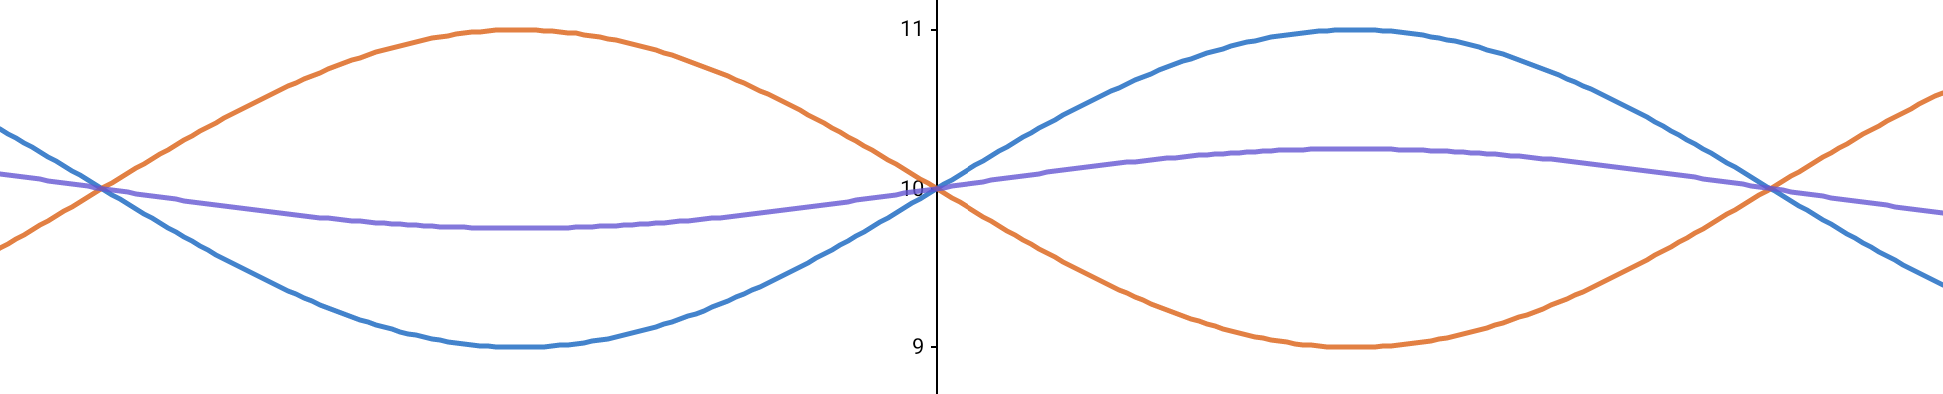
\includegraphics[width=0.6\textwidth, angle=0]{Grafico.png}
\end{center}
\end{figure}
\vspace{0.3cm}
\par Na imagem estão representados os gráficos de $\sin{x} + 10$, $-\sin{x} + 10$ e $\frac{1}{4}\sin{x} + 10$.
\par
\vspace{0.3cm}
\begin{flushleft}
Aplicações:
\par
\vspace{0.3cm}
1. Seja $f$ uma função definida em $\mathbb{R}$ tal que para todo $x\neq 1$, $-x^2 + 3x\leq f(x)\leq \frac{x^2 - 1}{x-1}$. Calcule $\displaystyle{\lim_{x\to 1}} f(x)$ e justifique.
\par
\vspace{0.3cm}
1.1 Resolução.
\end{flushleft}
\par Sejam $g(x)=-x^2 + 3x$ e $h(x)=\frac{x^2 - 1}{x-1}$. Sendo $\displaystyle{\lim_{x\to 1} g(x) = \lim_{x\to 1}} h(x) =2$, segue do Teorema do Confronto que $\displaystyle{\lim_{x\to 1}} f(x) = 2$.
\par
\vspace{0.3cm}
\begin{flushleft}
2. Sejam $f$ e $g$ duas funções com mesmo domínio $A$ tais que $\displaystyle{\lim_{x\to p}} f(x) = 0$ e $|g(x)|\leq M$ para todo $x$ em $A$, com $M>0$ fixo. Prove que $\displaystyle{\lim_{x\to p}} f(x)\cdot g(x) = 0$.
\end{flushleft}
\par
\vspace{0.3cm}
\begin{flushleft}
2.1 Demonstração.
\end{flushleft}
\par
Note que $|g(x)|\leq M \Rightarrow |g(x)|\cdot |f(x)|\leq M\cdot|f(x)|\Rightarrow -M\cdot|f(x)|\leq f(x)\cdot g(x)\leq M\cdot|f(x)|$.
\vspace{0.2cm}
\par Como $\displaystyle{\lim_{x\to p} (-M|f(x)| ) = \lim_{x\to p} (M |f(x)| ) = 0, \lim_{x\to p}} f(x)\cdot g(x) = 0$, pelo Teorema do Confronto.
\begin{flushright} $_{\blacksquare }$ \end{flushright}
\par
\vspace{0.3cm}
\begin{flushleft}
3. Prove que $\displaystyle{\lim_{x\to 0}} \frac{\sin{x}}{x} = 1$.
\end{flushleft}
\vspace{0.3cm}
\begin{flushleft}
3.1 Demonstração.
\end{flushleft}
\par
Vamos provar que $\displaystyle{\lim_{x\to 0^{-}}} \frac{\sin{x}}{x} = 1$ e $\displaystyle{\lim_{x\to 0^{+}}} \frac{\sin{x}}{x} = 1$.
\vspace{0.3cm}
\par
Admitindo que $0<x<\displaystyle{\frac{\pi }{2}}$ seja o ângulo $B\hat{A}C$, considere a figura abaixo, que simboliza o ciclo trigonométrico. Da figura segue que a área do $\triangle CAB$ é menor que a área do arco $B\hat{A}C$ que por sua vez é menor que a área do $\triangle ACE$.
\begin{figure}[htbp]
\begin{center}
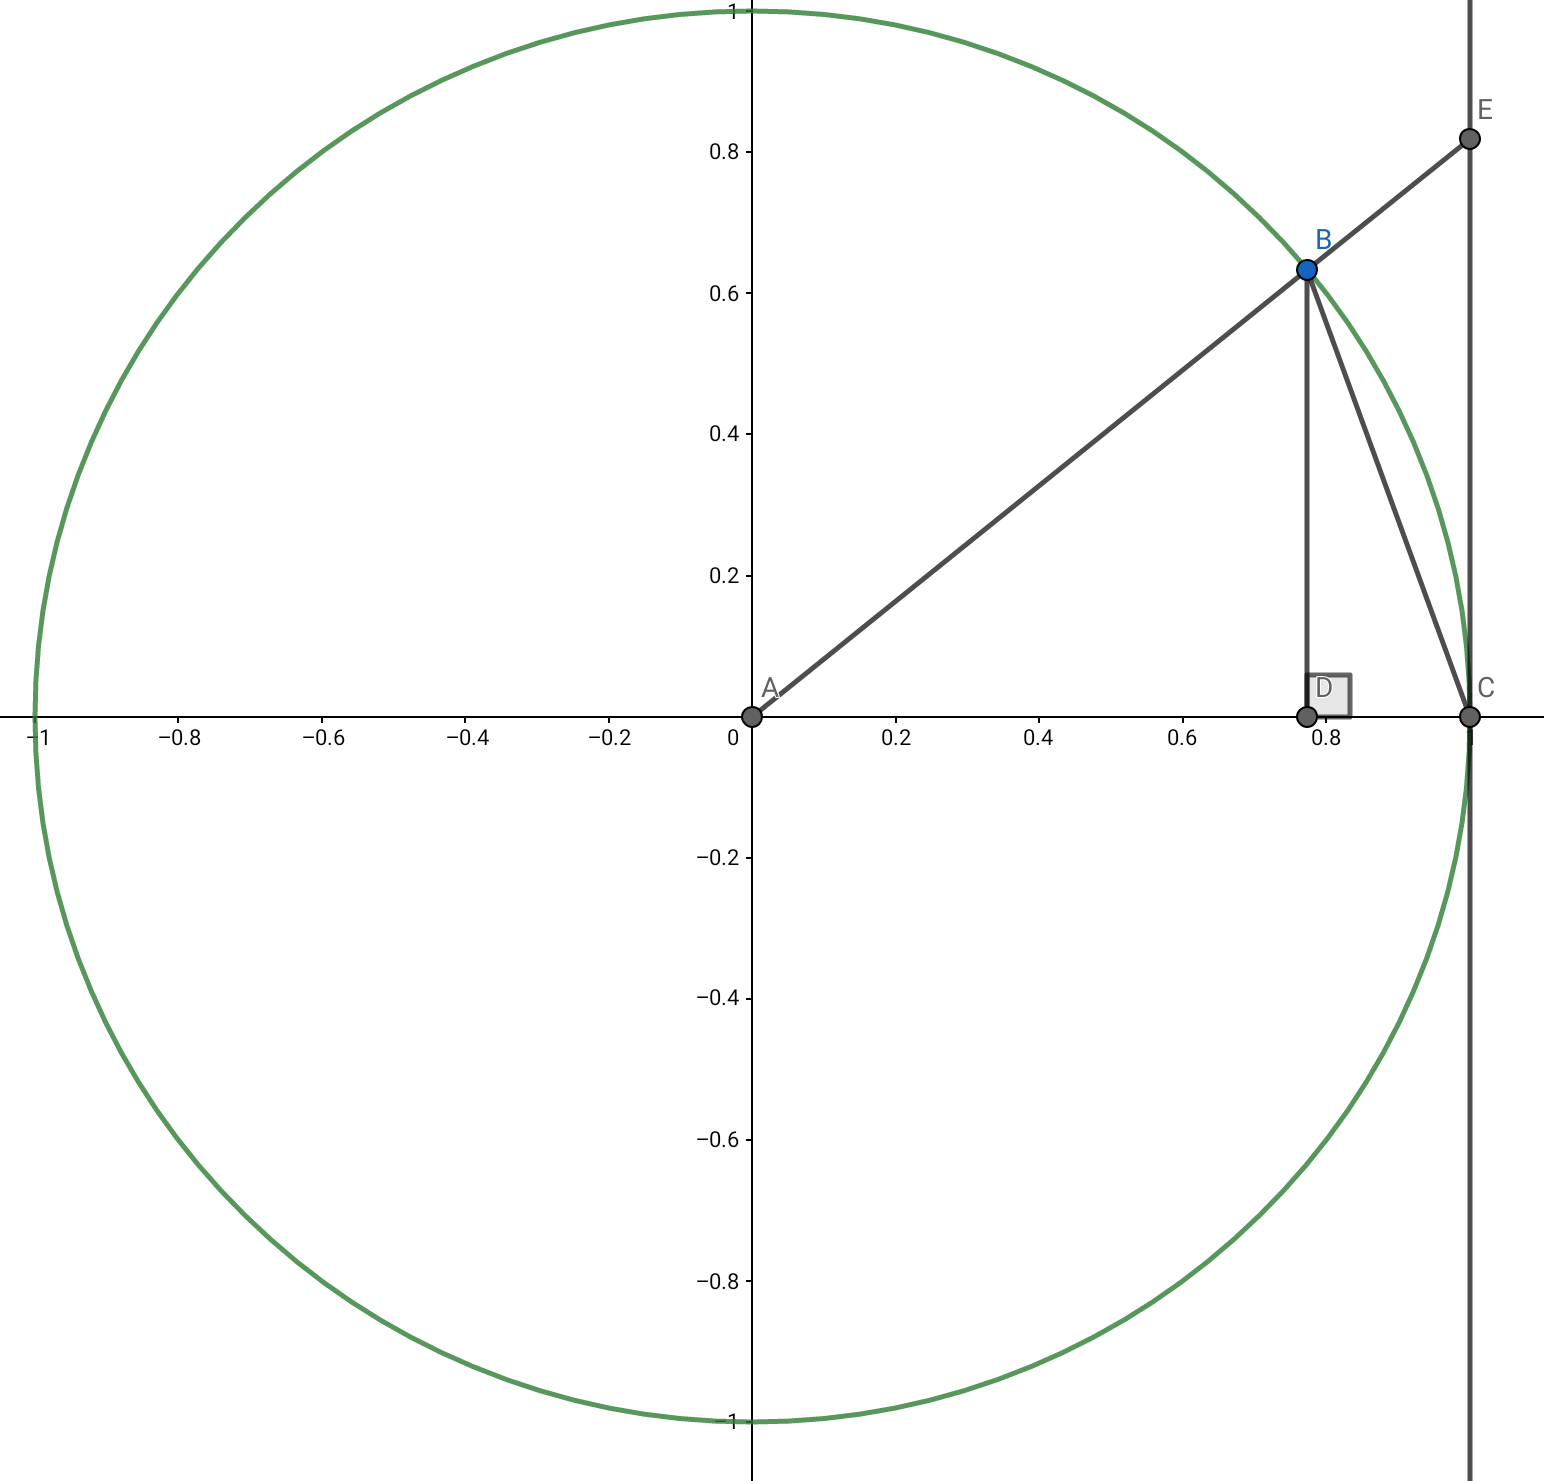
\includegraphics[width=0.6\textwidth, angle=0]{Circulo.png}
\end{center}
\end{figure}
\par
\vspace{0.3cm}
\begin{center} $\therefore\displaystyle{\frac{1\cdot\sin{x}}{2}<\frac{1^2\cdot x}{2}<\frac{1\cdot\tan{x}}{2}\Leftrightarrow\sin{x}<x<\tan{x}\Leftrightarrow 1<\frac{x}{\sin{x}}<\frac{1}{\cos{x}}\Leftrightarrow \cos{x}<\frac{\sin{x}}{x}}<1$.\end{center}
\par
\vspace{0.3cm}
Sendo $\displaystyle{\lim_{x\to 0^{+}} \cos{x} = \lim_{x\to 0^{+}} 1 = 1}$, segue pelo Teorema do Confronto que $\displaystyle{\lim_{x\to 0^{+}}} \frac{\sin{x}}{x} = 1$.
\par
\vspace{0.3cm}
Agora, para $\displaystyle{-\frac{\pi }{2}<x<0}$, temos $\displaystyle{0<-x<\frac{\pi }{2}}$. Daí,
\par
\vspace{0.3cm}
\begin{center}$\cos{(-x)}<\displaystyle{\frac{\sin{(-x)}}{-x}<1\Leftrightarrow \cos{x}<\frac{\sin{x}}{x}<1}$.\end{center}
\par
\vspace{0.3cm}
Sendo $\displaystyle{\lim_{x\to 0^{-}} \cos{x}=\lim_{x\to 0^{-}} 1 = 1}$ , temos, também pelo Teorema do Confronto, $\displaystyle{\lim_{x\to 0^{-}} \frac{\sin{x}}{x}} = 1$.
$$\therefore \displaystyle{\lim_{x\to 0}} \displaystyle{\frac{\sin{x}}{x}} = 1.$$ \begin{flushright} $_{\blacksquare }$ \end{flushright}
\par
\vspace{0.3cm}
\subsection{Limite exponencial fundamental - demonstração}
\par
\begin{flushleft} Admitindo que $\displaystyle{\lim_{x\to +\infty }} \Big(1 + \frac{1}{x}\Big)^x = e$, prove que:
\end{flushleft}
\par
\vspace{0.3cm}
a) $\displaystyle{\lim_{x\to -\infty }} \Big(1 + \frac{1}{x}\Big)^x = e$
\hspace{0.3cm}
b) $\displaystyle{\lim_{x\to 0}} \Big(1 + x\Big)^{\frac{1}{x}} = e$
\hspace{0.3cm}
c) $\displaystyle{\lim_{x\to 0}} \frac{a^x - 1}{x} = \ln{a}$, com $a>0$ fixo
\vspace{0.3cm}
\par
\textbf{Demonstração.}
\par
a) Seja $x=-(y+1)$. Então, $y=-x-1$ e quando $x\rightarrow -\infty $, $y\rightarrow +\infty $. Portanto,
\par
\vspace{0.3cm}
$ \displaystyle{\lim_{x\to -\infty }} \Big(1 + \frac{1}{x}\Big)^x = \displaystyle{\lim_{y\to +\infty }} \Big(1 + \frac{1}{-(y+1)}\Big)^{-(y+1)} = \displaystyle{\lim_{y\to +\infty }} \Big(\frac{y}{y+1}\Big)^{-(y+1)} = \displaystyle{\lim_{y\to +\infty }} \Big(\frac{y+1}{y}\Big)^{y+1} = $\par \vspace{0.2cm}$= \displaystyle{\lim_{y\to +\infty }} \Big(\frac{y+1}{y}\Big)^{y}\cdot \displaystyle{\lim_{y\to +\infty }} \Big(\frac{y+1}{y}\Big)^{1} = e\cdot1 = e$. \begin{flushright} $_{\blacksquare }$ \end{flushright}
\par
\vspace{0.3cm}
b) Tomando $x=\displaystyle{\frac{1}{y}}$, $x\rightarrow 0^{+}\Rightarrow y\rightarrow +\infty$, $x\rightarrow 0^{-}\Rightarrow y\rightarrow -\infty$, temos:
\par
\vspace{0.3cm}
$\displaystyle{\lim_{x\to 0^{+}}} \Big(1 + x\Big)^{\frac{1}{x}} =  \displaystyle{\lim_{y\to +\infty }} \Big(1 + \frac{1}{y}\Big)^{y} = e$\hspace{0.3cm} e
\hspace{0.3cm}
$\displaystyle{\lim_{x\to 0^{-}}} \Big(1 + x\Big)^{\frac{1}{x}} = \displaystyle{\lim_{y\to -\infty }} \Big(1 + \frac{1}{y}\Big)^{y} = e$.
\par
\vspace{0.3cm}
$$\therefore \displaystyle{\lim_{x\to 0}} \Big(1 + x\Big)^{\frac{1}{x}} = e.$$ \begin{flushright} $_{\blacksquare }$ \end{flushright}
\par
\vspace{0.3cm}
c) Consideraremos dois casos:
\par
1° caso) $a=1$.
\begin{center} $\displaystyle{\lim_{x\to 0}} \frac{a^x - 1}{x} = 0 = \ln{1}.$\end{center}
\par
\vspace{0.3cm}
2° caso) $a\neq 1$ e $a>0$.
\par Fazendo $a^x - 1=y$, $x\rightarrow 0\Rightarrow y\rightarrow 0$ e $x=\displaystyle{\frac{\ln{(1+y)}}{\ln{a}}}$. Logo, temos:
\begin{equation*} \displaystyle{\lim_{x\to 0}} \frac{a^x - 1}{x} = \displaystyle{\lim_{y\to 0}} \displaystyle{\frac{y}{\displaystyle{\frac{\ln{(1+y)}}{\ln{a}}}}} = \ln{(a)}\cdot\displaystyle{\lim_{y\to 0}} \displaystyle{\frac{y}{\ln{(1+y)}}} = \ln{(a)}\cdot \displaystyle{\lim_{y\to 0}} \displaystyle{\frac{1}{\ln{(1+y)^{\frac{1}{y}}}}} = \ln{(a)}\cdot\frac{1}{\ln{e}} = \ln{a}. \end{equation*} \begin{flushright} $_{\blacksquare }$ \end{flushright}
\par
\vspace{0.3cm}
\section{Derivada de uma função}
\subsection{Definição}
\hspace{12pt} Sejam $y=f(x)$ uma função e $p$ um ponto do domínio de $f$. O limite $\displaystyle{\lim_{x\to p}}\displaystyle{\frac{f(x)-f(p)}{x-p}}$, quando existe e é finito, é denominado derivada de $f$ em $p$.
\par O valor do limite $\displaystyle{\lim_{x\to p}}\displaystyle{\frac{f(x)-f(p)}{x-p}}$ é, em geral, indicado por $f'(p)$ ou $\displaystyle{\frac{dy}{dx}(p)}$, ou ainda, $y'(p)$.
\par A derivada de $y=f(x)$ em $p$, isto é, $f'(p)$, nos dá o coeficiente angular da reta tangente a curva de equação $y=f(x)$ no ponto $p$.
\par Outra interpretação possível para a derivada é valor instantâneo. Por exemplo, a derivada do espaço em função do tempo nos dá a velocidade instantânea num dado momento.
\par Note que, tomando $x-p=h$, temos:
$$ \displaystyle{\lim_{x\to p}}\displaystyle{\frac{f(x)-f(p)}{x-p}} = \displaystyle{\lim_{h\to 0}}\displaystyle{\frac{f(h+p)-f(p)}{h}}.$$
\par Os limites $\displaystyle{\lim_{x\to p^{+}}}\displaystyle{\frac{f(x)-f(p)}{x-p}}$ e $\displaystyle{\lim_{x\to p^{-}}}\displaystyle{\frac{f(x)-f(p)}{x-p}}$ são denominados, respectivamente, derivada lateral à direita ($f'_{+}(p)$) e derivada lateral à esquerda ($f'_{-}(p)$).
\par
\vspace{0.3cm}
Veja as derivadas de algumas funções elementares:
\par
\vspace{0.3cm}
1.$(c)'=0$, $\forall c\in\mathbb{R}$;
\par
\vspace{0.3cm}
2.$(x^n)'=n\cdot x^{n-1}$, $\forall n\in\mathbb{R}$;
\par
\vspace{0.3cm}
3.$(\sin{x})'=\cos{x}$, $\forall x\in\mathbb{R}$;
\par
\vspace{0.3cm}
4.$(\cos{x})'=-\sin{x}$, $\forall x\in\mathbb{R}$;
\par
\vspace{0.3cm}
5.$(\tan{x})'=\sec^{2}{x}$, $\forall x\in\mathbb{R}-\Big\{\displaystyle{\frac{\pi }{2}} + k\pi, k\in\mathbb{Z}\Big\}$;
\par
\vspace{0.3cm}
6.$(\cot{x})'=-\csc^{2}{x}$, $\forall x\in\mathbb{R}-\{{k\pi, k\in\mathbb{Z}}\}$;
\par
\vspace{0.3cm}
7.$(\sec{x})'=\sec{x}\cdot\tan{x}$, $\forall x\in\mathbb{R}-\Big\{\displaystyle{\frac{\pi }{2}} + k\pi, k\in\mathbb{Z}\Big\}$;
\par
\vspace{0.3cm}
8.$(\csc{x})'=-\csc{x}\cdot\cot{x}$, $\forall x\in\mathbb{R}-\{{k\pi, k\in\mathbb{Z}}\}$;
\par
\vspace{0.3cm}
9.$(\arcsin{x})'=\displaystyle{\displaystyle{\frac{1}{\sqrt{1-x^2}}}}$, $\forall x\in ]-1;1[$;
\par
\vspace{0.3cm}
10.$(\arccos{x})'=\displaystyle{\displaystyle{\frac{-1}{\sqrt{1-x^2}}}}$, $\forall x\in ]-1;1[$;
\par
\vspace{0.3cm}
11.$(\arctan{x})'=\displaystyle{\displaystyle{\frac{1}{1+x^2}}}$, $\forall x\in\mathbb{R}$;
\par
\vspace{0.3cm}
12.$(\operatorname{arccot(x)})'= \displaystyle{\displaystyle{\frac{-1}{1+x^2}}}$, $\forall x\in\mathbb{R}$;
\par
\vspace{0.3cm}
13.$(\operatorname{arcsec(x)})'= \displaystyle{\frac{1}{|x|\cdot\sqrt{x^2 - 1}}}$, $\forall x\in ]-\infty ;-1[ \cup ]1;+\infty[$;
\par
\vspace{0.3cm}
14.$(\operatorname{arccsc(x)})'= \displaystyle{\frac{-1}{|x|\cdot\sqrt{x^2 - 1}}}$, $\forall x\in ]-\infty ;-1[ \cup ]1;+\infty[$;
\par
\vspace{0.3cm}
15.$(a^x)'= a^{x}\cdot\ln{a}$, $\forall x\in\mathbb{R}$ e $a\in\mathbb{R}$ fixo;
\par
\vspace{0.3cm}
16.$(\log_{a}{x})'=\displaystyle{\frac{1}{x\cdot\ln{a}}}$, $\forall x\in\mathbb{R^{*}_{+}}$ e $0<a\neq1$ fixo.
\par
\vspace{0.3cm}
\subsection{Demonstrações das derivadas de algumas funções elementares}
\par
\vspace{0.3cm}
\begin{flushleft}
1. Função constante
\end{flushleft}
\par Se $f:\mathbb{R}\rightarrow\mathbb{R}$, com $f(x)=c$, $c\in\mathbb{R}$ fixo, tem-se:
\par $f'(x)=(c)'= \displaystyle{\lim_{h\to 0}} \displaystyle{\frac{f(x+h)-f(x)}{h}} = \displaystyle{\lim_{h\to 0}} \frac{c-c}{h} = 0. $ \begin{flushright} $_{\blacksquare }$ \end{flushright}
\par
\vspace{0.3cm}
\begin{flushleft}
2. Função potência
\end{flushleft}
\par Se $f:\mathbb{R}\rightarrow\mathbb{R}$, com $f(x)=x^n$, $n\in\mathbb{N}$ fixo, segue da definição de derivada:
\par $f'(x)=(x^n)'=\displaystyle{\lim_{y\to x}} \frac{f(y) - f(x)}{y-x}=\displaystyle{\lim_{y\to x}} \frac{y^n - x^n}{y-x}=\displaystyle{\lim_{y\to x}} \frac{(y-x)(y^{n-1}+xy^{n-2}+\cdots +x^{n-1})}{y-x}= $\par$ = \displaystyle{\lim_{y\to x}} x^{n-1}+x^{n-1}+\cdots +x^{n-1}=n\cdot x^{n-1}.$\begin{flushright}$\blacksquare $\end{flushright}
\par
\vspace{0.3cm}
\begin{flushleft}
3. Função seno
\end{flushleft}
\par Se $f:\mathbb{R}\rightarrow\mathbb{R}$, com $f(x)=\sin{x}$, segue da definição de derivada:
\par $f'(x)=(\sin{x})'=\displaystyle{\lim_{y\to x}} \frac{\sin{y} - \sin{x}}{y-x} = \displaystyle{\lim_{y\to x}} \displaystyle{\frac{2\cos{(\frac{x+y}{2})}\sin{(\frac{y-x}{2})}}{y-x}} = \displaystyle{\lim_{y\to x}} \cos{\Big(\frac{x+y}{2}\Big)}\cdot\frac{\sin{(\frac{y-x}{2})}}{\frac{y-x}{2}} = \cos{x}.$\begin{flushright} $_{\blacksquare }$ \end{flushright}
\par
\vspace{0.3cm}
\begin{flushleft}
4. Função cosseno
\end{flushleft}
\par Se $f:\mathbb{R}\rightarrow\mathbb{R}$, com $f(x)=\cos{x}$, segue da definição de derivada:
\par $f'(x)=(\cos{x})'=\displaystyle{\lim_{y\to x}} \frac{\cos{y} - \cos{x}}{y-x} = \displaystyle{\lim_{y\to x}} \frac{-2\sin{(\frac{y-x}{2})}\sin{(\frac{y+x}{2})}}{y-x} = \displaystyle{\lim_{y\to x}} -\sin{\Big(\frac{y+x}{2}\Big)}\cdot\frac{\sin{(\frac{y-x}{2})}}{\frac{y-x}{2}} = -\sin{x}.$ \begin{flushright} $_{\blacksquare }$ \end{flushright}
\par
\vspace{0.3cm}
\begin{flushleft}
5. Função tangente
\end{flushleft}
\par Se $f:\mathbb{R}-\Big\{\displaystyle{\frac{\pi }{2}} + k\pi, k\in\mathbb{Z}\Big\}\rightarrow\mathbb{R}$, $f(x)=\tan{x}$, vale:
\par $f'(x)=(\tan{x})'=\displaystyle{\lim_{y\to x}} \frac{\frac{\sin{y}}{\cos{y}} - \frac{\sin{x}}{\cos{x}}}{y-x} = \displaystyle{\lim_{y\to x}} \frac{\cos{x}\sin{y} - \cos{y}\sin{x}}{(y-x)(\cos{y}\cdot\cos{x})} = \displaystyle{\lim_{y\to x}} \frac{\sin{(y-x)}}{(y-x)}\cdot\frac{1}{\cos{y}\cos{x}} = \sec^2{x}.$\begin{flushright} $_{\blacksquare }$ \end{flushright}
\par
\vspace{0.3cm}
\begin{flushleft}
6. Função cotangente
\end{flushleft}
\par Se $f:\mathbb{R}-\{{k\pi, k\in\mathbb{Z}}\}\rightarrow\mathbb{R}$, $f(x)=\cot{x}$, tem-se:
\par $f'(x)=(\cot{x})'=\displaystyle{\lim_{y\to x}} \frac{\frac{\cos{y}}{\sin{y}} - \frac{\cos{x}}{\sin{x}}}{y-x} = \displaystyle{\lim_{y\to x}} \frac{\cos{y}\sin{x} - \cos{x}\sin{y}}{(y-x)(\sin{x}\sin{y})} = \displaystyle{\lim_{y\to x}} \frac{\sin{(x-y)}}{(x-y)(-\sin{x}\sin{y})} = -\csc^2{x}.$\begin{flushright} $_{\blacksquare }$ \end{flushright}
\par
\vspace{0.3cm}
\begin{flushleft}
7. Função secante
\end{flushleft}
\par Se $f:\mathbb{R}-\Big\{\displaystyle{\frac{\pi }{2}} + k\pi, k\in\mathbb{Z}\Big\}\rightarrow\mathbb{R}$, $f(x)=\sec{x}$, obtemos:
\par $ f'(x)=(\sec{x})'=\displaystyle{\lim_{y\to x}} \frac{\frac{1}{\cos{y}} - \frac{1}{\cos{x}}}{y-x} = \displaystyle{\lim_{y\to x}} \frac{\cos{x} - \cos{y}}{(y-x)(\cos{y}\cos{x})} =  \displaystyle{\lim_{y\to x}} \frac{-2\sin{(\frac{x+y}{2})}\sin{(\frac{x-y}{2})}}{-(x-y)(\cos{y}\cos{x})} =$\par \vspace{0.2cm}$= \displaystyle{\lim_{y\to x}} \frac{\sin{(\frac{x-y}{2})}}{\frac{x-y}{2}}\cdot\frac{\sin{(\frac{x+y}{2})}}{\cos{y}\cos{x}} = \frac{\sin{x}}{\cos^2{x}} = \sec{x}\tan{x}.$ \begin{flushright} $_{\blacksquare }$ \end{flushright}
\par
\vspace{0.3cm}
\begin{flushleft}
8. Função cossecante
\end{flushleft}
\par Se $f:\mathbb{R}-\{{k\pi, k\in\mathbb{Z}}\}\rightarrow\mathbb{R}$, $f(x)=\csc{x}$, temos:
\par $f'(x)=(\csc{x})'=\displaystyle{\lim_{y\to x}} \frac{\frac{1}{\sin{y}} - \frac{1}{\sin{x}}}{y-x} = \displaystyle{\lim_{y\to x}} \frac{\sin{x} - \sin{y}}{(y-x)(\sin{y}\sin{x})} = \displaystyle{\lim_{y\to x}} \frac{2\sin{(\frac{x-y}{2})}\cos{(\frac{x+y}{2})}}{-(x-y)(\sin{y}\sin{x})} = \frac{-\cos{x}}{\sin^2{x}} = $\vspace{0.2cm} $-\csc{x}\cot{x}.$\begin{flushright} $_{\blacksquare }$ \end{flushright}
\par
\vspace{0.3cm}
\begin{flushleft}
9. Função arcoseno
\end{flushleft}
\par Se $f:]-1;1[\rightarrow\mathbb{R}$, $f(x)=\arcsin{x}$, podemos escrever:
\par \begin{center} $\arcsin{x}=z\Leftrightarrow x=\sin{z}$ e $\arcsin{y}=w\Leftrightarrow y=\sin{w}$.\end{center}
\vspace{0.3cm}
\par Portanto, segue da definição derivada:
\par $f'(x)=(\arcsin{x})'=\displaystyle{\lim_{y\to x}} \frac{\arcsin{y} - \arcsin{x}}{y-x}=\displaystyle{\lim_{w\to z}} \frac{w-z}{\sin{w} - \sin{z}} = \displaystyle{\lim_{w\to z}} \frac{\frac{w-z}{2}}{\sin{(\frac{w-z}{2})}\cos{(\frac{w+z}{2})}} = \frac{1}{\cos{z}}$.
\vspace{0.3cm}
\par Contudo, $x=\sin{z}\Rightarrow x^2=1-\cos^2{z}\Rightarrow \cos^2{z}=1-x^2\Rightarrow \cos{z}=\sqrt{1-x^2}$, pois $\displaystyle{\frac{-\pi }{2}} < z < \displaystyle{\frac{\pi }{2}}$, logo $\cos{z} > 0$.
\vspace{0.3cm}
$$\therefore (\arcsin{x})'=\frac{1}{\cos{z}}=\frac{1}{\sqrt{1-x^2}}.$$\begin{flushright} $_{\blacksquare }$ \end{flushright}
\par
\vspace{0.3cm}
\begin{flushleft}
10. Função arcocosseno
\end{flushleft}
\par Se $f:]-1;1[\rightarrow\mathbb{R}$, $f(x)=\arccos{x}$, podemos escrever:
\par \begin{center} $\arccos{x}=a\Leftrightarrow x=\cos{a}$ e $\arccos{y}=b\Leftrightarrow y=\cos{b}$.\end{center}
\vspace{0.3cm}
\par Portanto, segue da definição derivada:
\par $f'(x)=(\arccos{x})'=\displaystyle{\lim_{y\to x}} \frac{\arccos{y} - \arccos{x}}{y-x}=\displaystyle{\lim_{b\to a}} \frac{b-a}{\cos{b} - \cos{a}} = \displaystyle{\lim_{b\to a}} \frac{\frac{b-a}{2}}{-\sin{(\frac{b-a}{2})}\sin{(\frac{b+a}{2})}} = \frac{-1}{\sin{a}}$.
\vspace{0.3cm}
\par Contudo, $x=\cos{a}\Rightarrow x^2=1-\sin^2{a}\Rightarrow \sin^2{a}=1-x^2\Rightarrow \sin{a}=\sqrt{1-x^2}$, pois $0 < a < \pi$, logo $\sin{a}> 0$.
\vspace{0.3cm}
$$\therefore (\arccos{x})'=\frac{-1}{\sin{a}}=\frac{-1}{\sqrt{1-x^2}}.$$
\begin{flushright} $_{\blacksquare }$ \end{flushright}
\par
\vspace{0.3cm}
\begin{flushleft}
11. Função arcotangente
\end{flushleft}
\par Se $f:\mathbb{R}\rightarrow\mathbb{R}$, $f(x)=\arctan{x}$, podemos dizer:
\par \begin{center} $\arctan{x}=\alpha\Leftrightarrow x=\tan{\alpha }$ e  $\arctan{y}=\beta\Leftrightarrow y=\tan{\beta }$.\end{center}
\vspace{0.3cm}
\par Logo, segue da definição de derivada:
\par $f'(x)=(\arctan{x})'=\displaystyle{\lim_{y\to x}} \frac{\arctan{y} - \arctan{x}}{y-x} = \displaystyle{\lim_{\beta\to \alpha }} \frac{\beta - \alpha }{\tan{\beta } - \tan{\alpha }} = \displaystyle{\lim_{\beta\to \alpha }} \frac{\beta - \alpha }{\frac{\sin{(\beta - \alpha )}}{\cos{\beta }\cos{\alpha }}} = \cos^2{\alpha }$.
\vspace{0.3cm}
\par Note que $x=\tan{\alpha }\Rightarrow x^2=\displaystyle{\frac{1}{\cos^2{\alpha }} - 1 \Rightarrow \cos^2{\alpha }=\frac{1}{1+x^2}}$.
\vspace{0.3cm}
$$\therefore (\arctan{x})'=\cos^2{\alpha }=\frac{1}{1+x^2}.$$
\begin{flushright} $_{\blacksquare }$ \end{flushright}
\par
\vspace{0.3cm}
\begin{flushleft}
12. Função arcocotangente
\end{flushleft}
\par Se $f:\mathbb{R}\rightarrow\mathbb{R}$, $f(x)=\operatorname{arccot(x)}$, pode-se escrever:
\par \begin{center} $\operatorname{arccot(x)}=a\Leftrightarrow x=\cot{a}$ e $\operatorname{arccot(y)}=b\Leftrightarrow y=\cot{b}$.\end{center}
\vspace{0.3cm}
\par Segue da definição de derivada:
\par $f'(x)=(\operatorname{arccot(x)})'=\displaystyle{\lim_{y\to x}} \frac{\operatorname{arccot(y)} - \operatorname{arccot(x)}}{y-x} = \displaystyle{\lim_{b\to a}} \frac{b-a}{\frac{-\sin{(b-a)}}{\sin{a}\sin{b}}} = -\sin^2{a}$.
\vspace{0.3cm}
\par Contudo, $x=\cot{a}\Rightarrow x^2 =\displaystyle{\frac{1}{\sin^2{a}} - 1\Rightarrow \sin^2{a}=\frac{1}{1+x^2}}$.
\vspace{0.3cm}
$$\therefore (\operatorname{arccot(x)})' = -\sin^2{a} =\frac{-1}{1+x^2}.$$
\begin{flushright} $_{\blacksquare }$ \end{flushright}
\par
\vspace{0.3cm}
\begin{flushleft}
13. Função arcosecante
\end{flushleft}
\par Se $f:]-\infty ;-1[ \cup ]1;+\infty[\rightarrow\mathbb{R}$, $f(x)=\operatorname{arcsec(x)}$, podemos escrever:
\par \begin{center} $\operatorname{arcsec(x)} = w\Leftrightarrow x=\sec{w}$ e $\operatorname{arcsec(y)}=z\Leftrightarrow y=\sec{z}$.\end{center}
\vspace{0.3cm}
\par Segue da definição de derivada:
\par $f'(x)=(\operatorname{arcsec(x)})'=\displaystyle{\lim_{y\to x}} \frac{\operatorname{arcsec(y)} - \operatorname{arcsec(x)}}{y-x} =  \displaystyle{\lim_{z\to w}} \frac{z-w}{\frac{1}{\cos{z}} - \frac{1}{\cos{w}}} = \displaystyle{\lim_{z\to w}} \frac{\frac{w-z}{2}}{\frac{\sin{(\frac{w-z}{2})}\sin{(\frac{w+z}{2})}}{\cos{z}\cos{w}}} = \frac{\cos^2{w}}{\sin{w}}$.
\vspace{0.3cm}
\par Porém, por um lado $x=\sec{w}\Rightarrow\displaystyle{x^2=\frac{1}{\cos^2{w}}\Rightarrow \cos^2{w}=\frac{1}{x^2}}$.
\vspace{0.3cm}
\par Por outro lado, $\displaystyle{\cos^2{w}=\frac{1}{x^2}\Rightarrow \sin^2{w}=1-\frac{1}{x^2}\Rightarrow \sin{w}=\sqrt{\frac{x^2 - 1}{x^2}}}$, uma vez que $0<w<\pi$, $w\neq\displaystyle{\frac{\pi}{2}}$, logo $\sin{w}>0$.
\vspace{0.3cm}
$$\therefore (\operatorname{arcsec(x)})'=\frac{\cos^2{w}}{\sin{w}}=\frac{1}{x^2\sqrt{\frac{x^2 - 1}{x^2}}} =\frac{|x|}{x^2\cdot\sqrt{x^2 - 1}} = \frac{1}{|x|\cdot\sqrt{x^2-1}}.$$
\begin{flushright} $_{\blacksquare }$ \end{flushright}
\par
\vspace{0.3cm}
\begin{flushleft}
14. Função arcocossecante
\end{flushleft}
\par Se $f:]-\infty ;-1[ \cup ]1;+\infty[\rightarrow\mathbb{R}$, $f(x)=\operatorname{arccsc(x)}$, podemos escrever:
\par \begin{center} $\operatorname{arccsc(x)} = a\Leftrightarrow x=\csc{a}$ e $\operatorname{arccsc(y)}=b\Leftrightarrow y=\csc{b}$.\end{center}
\vspace{0.3cm}
\par Segue da definição de derivada:
\par $f'(x)=(\operatorname{arccsc(x)})'=\displaystyle{\lim_{y\to x}} \frac{\operatorname{arccsc(y)} - \operatorname{arccsc(x)}}{y-x} =  \displaystyle{\lim_{b\to a}} \frac{b-a}{\frac{1}{\sin{b}} - \frac{1}{\sin{a}}} = \displaystyle{\lim_{b\to a}} \frac{\frac{-(a-b)}{2}}{\frac{\sin{(\frac{a-b}{2})}\cos{(\frac{a+b}{2})}}{\sin{b}\sin{a}}} = \frac{-\sin^2{a}}{\cos{a}}$.
\vspace{0.3cm}
\par Porém, por um lado $x=\csc{a}\Rightarrow\displaystyle{x^2=\frac{1}{\sin^2{a}}\Rightarrow \sin^2{a}=\frac{1}{x^2}}$.
\vspace{0.3cm}
\par Por outro lado, $\sin^2{a}=\displaystyle{\frac{1}{x^2}\Rightarrow \cos^2{a}=1-\frac{1}{x^2}\Rightarrow \cos{a}=\sqrt{\frac{x^2 - 1}{x^2}}}$, uma vez que $\displaystyle{-\frac{\pi }{2}<a<\frac{\pi }{2}}$, $a\neq 0$, temos $\cos{a}>0$.
\vspace{0.3cm}
$$\therefore (\operatorname{arccsc(x)})'=\frac{-\sin^2{a}}{\cos{a}}=\frac{-1}{x^2\sqrt{\frac{x^2 - 1}{x^2}}} =\frac{-|x|}{x^2\cdot\sqrt{x^2 - 1}} = \frac{-1}{|x|\cdot\sqrt{x^2-1}}.$$
\begin{flushright} $_{\blacksquare }$ \end{flushright}
\par
\vspace{0.3cm}
\begin{flushleft}
15. Função exponencial
\end{flushleft}
\par Se $f:\mathbb{R}\rightarrow\mathbb{R}$, $f(x)=a^x$, segue da definição de derivada:
\par $f'(x)=(a^x)'=\displaystyle{\lim_{h\to 0}} \frac{a^{x+h} - a^x}{h} = a^x\displaystyle{\lim_{h\to 0} \frac{a^h - 1}{h}} = a^x\cdot\ln{a}.$\begin{flushright} $_{\blacksquare }$ \end{flushright}
\par
\vspace{0.3cm}
\begin{flushleft}
16. Função logarítmica
\end{flushleft}
\par Se $f:\mathbb{R^{*}_{+}}\rightarrow\mathbb{R}$, $f(x)=\log_{a}{x}$, temos, pela definição de derivada:
\par $f'(x)=(\log_{a}{x})'=\displaystyle{\lim_{h\to 0} \frac{\log_{a}{(h+x)} - \log_{a}{x}}{h}} = \displaystyle{\lim_{h\to 0} \log_{a}{\Big(1+\frac{h}{x}\Big)^{\frac{1}{h}}} = \log_{a}{e^{\frac{1}{x}}}} = \frac{1}{x\cdot\ln{a}}$.\begin{flushright} $_{\blacksquare }$ \end{flushright}
\par
\vspace{0.3cm}
\subsection{Regra de derivação do produto de duas funções}
\par\hspace{12pt}Sejam $f(x)$ e $g(x)$ duas funções. Vamos provar que a derivada de seu produto, $(f\cdot g)'(x)$, é igual a $$f'(x)\cdot g(x) + f(x)\cdot g'(x).$$
\par
\vspace{0.3cm}
\par
\textbf{Demonstração.}
\par
Da definição, decorre:
\vspace{0.3cm}

\begin{equation*}\begin{split}
(f\cdot g)'(x)&=\lim_{h\to 0}\frac{f(x+h)g(x+h)-f(x)g(x)}{h} =\\
&=\lim_{h\to 0} \frac{f(x+h)g(x+h) - f(x)g(x+h) + f(x)g(x+h) - f(x)g(x)}{h}=\\   
&=\lim_{h\to 0} \Big[g(x+h)\Big(\frac{f(x+h) - f(x)}{h}\Big)  +f(x)\Big(\frac{g(x+h) - g(x)}{h}\Big)\Big] = f'(x)g(x) + f(x)g'(x).
\end{split}
\end{equation*}
\begin{flushright} $_{\blacksquare}$ \end{flushright}
\vspace{0.3cm}
\subsection{Regra de derivação do quociente de duas funções}
\hspace{12pt}Sejam $f(x)$ e $g(x)$ duas funções. Vamos mostrar que a derivada de seu quociente, $\Big(\displaystyle{\frac{f}{g}}\Big)'(x)$, é igual a $$\displaystyle{\frac{f'(x)g(x) - f(x)g'(x)}{g^2(x)}}.$$
\vspace{0.3cm}
\par
\textbf{Demonstração.}
\par
Da definição, com $g(x)\neq 0$, segue:
\vspace{0.3cm}
\begin{equation*} \begin{split} \Big(\displaystyle{\frac{f}{g}}\Big)'(x) &= \displaystyle{\lim_{h\to 0} \frac{1}{h}\Big[\displaystyle{\frac{f(x+h)}{g(x+h)} - \frac{f(x)}{g(x)}}\Big]} = \\ &= \displaystyle{\lim_{h\to 0} \frac{1}{h}\cdot\displaystyle{\frac{f(x+h)g(x) - f(x)g(x+h)}{g(x+h)g(x)}}} =\\ &=
\displaystyle{\lim_{h\to 0} \frac{1}{h}\cdot\displaystyle{\frac{f(x+h)g(x) - f(x)g(x) + f(x)g(x) - f(x)g(x+h)}{g(x+h)g(x)}}} =\\ & = \displaystyle{\lim_{h\to 0} \frac{1}{g(x+h)g(x)}\Big[\displaystyle{g(x)\Big(\frac{f(x+h) - f(x)}{h}\Big) - f(x)\Big(\frac{g(x+h) - g(x)}{h}\Big)}\Big]} = \\ &= \displaystyle{\frac{f'(x)g(x) - f(x)g'(x)}{g^2(x)}} .\end{split} \end{equation*}\begin{flushright} $_{\blacksquare }$ \end{flushright}
\vspace{0.3cm}
\subsection{Exercícios iniciais - derivada}
\par
\vspace{0.3cm}
\begin{flushleft}
1. Determine a primeira derivada das funções:
\end{flushleft}
\par
\begin{multicols}{3}
\hspace{-15pt}a) $y=\displaystyle{\frac{x^3 + 7}{x}}$\\
b) $s=\displaystyle{\frac{t^2 + 5t - 1}{t^2}}$\\
c) $r=\displaystyle{\frac{(\theta - 1)(\theta^{2} + \theta + 1)}{\theta^{3}}}$\\
d) $w=(3-z)\bigg(\displaystyle{\frac{1+3z}{3z}}\bigg)$ \\
e) $w=e^{z}(z-1)(z^2 - 1)$\\
f) $p=\displaystyle{\frac{q^2 + 3}{(q-1)^3 + (q+1)^3}}$\\
g) $r=\displaystyle{\frac{12}{\theta }} - \displaystyle{\frac{4}{\theta^{3}}} + \displaystyle{\frac{1}{\theta^{4}}}$\\
h) $r=e^{\theta }\Big(\displaystyle{\frac{1}{\theta^{2}}} + \theta^{-\frac{\pi }{2}}\Big)$ \\
i) $r=\displaystyle{\frac{e^s}{s}}$
\end{multicols}
\par
\vspace{0.3cm}
\begin{flushleft}
1.1 Resolução.
\end{flushleft}
\par
a) $y=\displaystyle{\frac{x^3 + 7}{x}}\Rightarrow y=x^2 + 7x^{-1} \Rightarrow y'=2x-7x^{-2} \Rightarrow y'=2x-\displaystyle{\frac{7}{x^2}}        $.
\par
\vspace{0.3cm}
b) $s=\displaystyle{\frac{t^2 + 5t - 1}{t^2}} \Rightarrow s=1 + 5t^{-1} - t^{-2} \Rightarrow s'=-5t^{-2} + 2t^{-3} \Rightarrow s'=-\displaystyle{\frac{5}{t^2}} + \displaystyle{\frac{2}{t^3}}$.
\par
\vspace{0.3cm}
c) $r=\displaystyle{\frac{(\theta - 1)(\theta^{2} + \theta + 1)}{\theta^{3}}} \Rightarrow r=\displaystyle{\frac{\theta^{3} - 1}{\theta^{3}}} \Rightarrow r=1-\theta^{-3} \Rightarrow r'=3\theta^{-4} = \displaystyle{\frac{3}{\theta^{4}}}$.
\par
\vspace{0.3cm}
d) $w=(3-z)\displaystyle{\frac{1+3z}{3z}} \Rightarrow w=\displaystyle{\frac{-3z^2 + 8z + 3}{3z}} \Rightarrow w=-z + \frac{8}{3} + z^{-1} \Rightarrow w'=-1-z^{-2} = -1 - \displaystyle{\frac{1}{z^2}}$.
\par
\vspace{0.3cm}
e) $ w=e^{z}(z-1)(z^2 - 1) \Rightarrow w' = (e^z)'(z-1)(z^2 - 1) + (e^z)(z-1)'(z^2 - 1) + (e^z)(z-1)(z^2 - 1)' $\par $ \Rightarrow w' = e^z(z-1)(z^{2}-1) + e^z(z^{2}-1) + e^z(z-1)2z \Rightarrow w' = e^z(z^3 + 2z^2 - z)$.
\par
\vspace{0.3cm}
f) $p=\displaystyle{\frac{q^2 + 3}{(q-1)^3 + (q+1)^3}} \Rightarrow p=\displaystyle{\frac{q^2 + 3}{2q^3 + 6q}} \Rightarrow p = \displaystyle{\frac{1}{2q}} = \frac{1}{2}\cdot q^{-1} \Rightarrow p'=-\displaystyle{\frac{1}{2q^2}}$.
\par
\vspace{0.3cm}
g) $r=\displaystyle{\frac{12}{\theta }} - \displaystyle{\frac{4}{\theta^{3}}} + \displaystyle{\frac{1}{\theta^{4}}} \Rightarrow r=12\theta^{-1} - 4\theta^{-3} + \theta^{-4} \Rightarrow r'=-12\theta^{-2} + 12\theta^{-4} - 4\theta^{-5} = -\displaystyle{\frac{12}{\theta^{2}}} + \displaystyle{\frac{12}{\theta^{4}}} - \displaystyle{\frac{4}{\theta^{5}}}$.
\par
\vspace{0.3cm}
h) $r=e^{\theta }\Big(\displaystyle{\frac{1}{\theta^{2}}} + \theta^{-\frac{\pi }{2}}\Big) \Rightarrow r=e^{\theta }\Big(\theta^{-2} + \theta^{-\frac{\pi }{2}}\Big) \Rightarrow r'=(e^{\theta })'(\theta^{-2} + \theta^{-\frac{\pi }{2}}) + (e^{\theta })(\theta^{-2} + \theta^{-\frac{\pi }{2}})' $\par $\Rightarrow r'=e^{\theta }\Big(\displaystyle{\frac{1}{\theta^{2}}} + \displaystyle{\frac{1}{\theta^{\frac{\pi }{2}}}} - \displaystyle{\frac{2}{\theta^{3}}} - \displaystyle{\frac{\pi }{2\theta^{\frac{\pi }{2} + 1}}}\Big)$.
\par
\vspace{0.3cm}
i) $r=\displaystyle{\frac{e^s}{s}} \Rightarrow r'=\displaystyle{\frac{(e^{s})'s - e^{s}s'}{s^2}} \Rightarrow r'=\displaystyle{\frac{e^{s}(s-1)}{s^2}}$.
\par
\vspace{0.3cm}
\begin{flushleft}
2. Se um gás for mantido em um cilindro a uma temperatura constante $T$, a pressão $P$ estará relacionada com o volume $V$ de acordo com uma fórmula da forma $$P=\displaystyle{\frac{nRT}{V-nb}} - \displaystyle{\frac{an^2}{V}}$$ em que $a$, $b$, $n$ e $R$ são constantes. Determine $\displaystyle{\frac{dP}{dV}}$.
\end{flushleft}
\vspace{0.3cm}
\begin{flushleft}
2.1 Resolução.
\end{flushleft}
\par Utilizando as regras de derivação, vem:
\begin{equation*} \displaystyle{\frac{dP}{dV}} = nRT[(V-nb)^{-1}]' - an^{2}(V^{-1})' = -\displaystyle{\frac{nRT}{(V-nb)^2}} + \displaystyle{\frac{an^2}{V^2}} .\end{equation*}
\par
\vspace{0.3cm}
\subsection{Regra da Cadeia - regra para derivar uma função composta}
\par
\hspace{12pt}Se $y=f(x)$ é derivável no ponto $u=g(x)$ e $g(x)$ é derivável em $x$, então a função composta $y=f(g(x))$ é derivável em $x$ e vale a regra da cadeia:
$$y'=(f(g(x)))'=f'(g(x))\cdot g'(x)$$
\begin{center} ou, na notação de Leibniz, \end{center}
$$\displaystyle{\frac{dy}{dx}}=\displaystyle{\frac{dy}{du}}\cdot\displaystyle{\frac{du}{dx}}.$$
\par
\vspace{0.3cm}
\begin{flushleft}
Exemplos.
\par
\vspace{0.3cm}
1. Calcule $y'$:
\end{flushleft}
\par
\begin{multicols}{5}
a) $y=e^{3x}$\\
b) $y=(3x^2 +1)^3$\\
\hspace{15pt}c) $y=\cos{3x}$\\
d) $y=\sqrt[3]{x^2 + 3}$\\
e) $y=\ln{(x^2 + 3)}$
\end{multicols}
\par
\vspace{0.3cm}
\begin{flushleft}
1.1 Resolução.
\end{flushleft}
\par
a) Tomando $u=3x$, temos:
\begin{equation*} y=e^{u}\Rightarrow y'=u'\cdot (e^{u})' \Rightarrow y'=3\cdot e^{3x} .\end{equation*}
\par
\vspace{0.2cm}
\textbf{Regra geral}: $(e^{f(x)})'=e^{f(x)}\cdot f(x)$ e $(a^{f(x)})'=a^{f(x)}\cdot f'(x)\cdot \ln{a}$.
\par
\vspace{0.3cm}
b) Tome $3x^2 + 1=u$. Logo:
\begin{equation*} y=u^3 \Rightarrow y'=3u{^2}\cdot u' \Rightarrow y'=18x(3x^2 + 1)^{2}. \end{equation*}
\par
\vspace{0.2cm}
\textbf{Regra geral}: $[(f(x))^n]'=n\cdot (f(x))^{n-1}\cdot f'(x), \forall n\in\mathbb{R}$ fixo.
\par
\vspace{0.3cm}
c) Tomando-se $u=3x$, vem:
\begin{equation*} y=\cos{u} \Rightarrow y'=-\sin{u}\cdot u' \Rightarrow y'=-3\sin{3x}. \end{equation*}
\par
\vspace{0.2cm}
\textbf{Regra geral}: $(\cos{(f(x))})'=-\sin{(f(x))}\cdot f'(x)$ e $ (\cos^{n}{(f(x)})'=-n\cdot \cos^{n-1}{(f(x))}\cdot\sin{(f(x))}\cdot f'(x) $, $\forall n\in\mathbb{R}$ fixo.
\par
\vspace{0.3cm}
d) Tomando $u=x^2 + 3$, segue:
\begin{equation*} y=(u)^{\frac{1}{3}} \Rightarrow y'=\displaystyle{\frac{1}{3}}\cdot u^{-\frac{2}{3}}\cdot u' \Rightarrow y'=\displaystyle{\frac{2x}{3}}\cdot \displaystyle{\frac{1}{\sqrt[3]{(x^2 + 3)^2}}}. \end{equation*}
\par
\vspace{0.3cm}
e) Tomando-se $u=x^2 + 3$, temos:
\begin{equation*} y=\ln{u} \Rightarrow y'=\displaystyle{\frac{1}{u}}\cdot u' \Rightarrow y'=\displaystyle{\frac{2x}{x^2 + 3}}. \end{equation*}
\par
\vspace{0.2cm}
\textbf{Regra geral}: $[\ln{(f(x))}]'=\displaystyle{\frac{f'(x)}{f(x)}}$ e $[\log_{a}{(f(x))}]'=\displaystyle{\frac{f'(x)}{f(x)\cdot \ln{a}}}$.
\par
\vspace{0.3cm}
\begin{flushleft}
2. Seja $f:\mathbb{R}\rightarrow\mathbb{R}$ derivável e $g(t) = f(t^2 + 1)$. Supondo que $f'(2)=5$, calcule $g'(1)$.
\end{flushleft}
\vspace{0.3cm}
\begin{flushleft}
2.1 Resolução.
\end{flushleft}
\begin{equation*} g(t) = f(t^2 + 1) \Rightarrow g'(t)=f'(t^2 + 1) \Rightarrow g'(t)=2t\cdot f'(t^2 +1) .\end{equation*}
$$\therefore g'(1)=2\cdot f'(2) = 10.$$
\par
\vspace{0.3cm}
\textbf{Observação - Derivada de ordem superior}: Satisfeitas as condições de existência, valem as seguintes notações para as derivadas de $y=f(x)$:
\begin{itemize}
\item \textbf{derivada de ordem 1 ou primeira derivada}: $y'$ ou $\displaystyle{\frac{dy}{dx}}$
\item \textbf{derivada de ordem 2 ou segunda derivada}: $y''$ ou $\displaystyle{\frac{d^{2}y}{dx^2}}$
\item \textbf{derivada de ordem 3 ou terceira derivada}: $\overset{(3)}{y}$ ou $\displaystyle{\frac{d^{3}y}{dx^3}}$
\item \textbf{derivada de ordem n ou derivada n-ésima}: $\overset{(n)}{y}$ ou $\displaystyle{\frac{d^{n}y}{dx^n}}$
\end{itemize}
\vspace{0.3cm}
\begin{flushleft}
3. Seja $y=\sqrt{x^2 +1}$. Verifique que $\Big(\displaystyle{\frac{dy}{dx}}\Big)^2 + y\cdot\displaystyle{\frac{d^{2}y}{dx^2}} = 1.$
\end{flushleft}
\vspace{0.3cm}
\begin{flushleft}
3.1 Resolução.
\end{flushleft}
\par Vamos calcular $\displaystyle{\frac{dy}{dx}}$ e $\displaystyle{\frac{d^{2}y}{dx^2}}$.
\begin{equation*} \displaystyle{\frac{dy}{dx} = \frac{2x}{2\sqrt{x^2 + 1}} = x(x^2 + 1)^{-\frac{1}{2}}}. \end{equation*}
\begin{equation*} \displaystyle{\frac{d^{2}y}{dx^2} = (x^2 + 1)^{-\frac{1}{2}} - \frac{1}{2}\cdot (x^2 + 1)^{-\frac{3}{2}} \cdot 2x\cdot x = (x^2 + 1)^{-\frac{1}{2}} - x^{2}(x^2 + 1)^{-\frac{3}{2}}}. \end{equation*}
\vspace{0.2cm}
\par Logo,
\begin{equation*} \Big(\displaystyle{\frac{dy}{dx}}\Big)^2 + y\cdot\displaystyle{\frac{d^{2}y}{dx^2}} = \displaystyle{x^2\cdot (x^2 + 1)^{-1} - x^2\cdot (x^2 + 1)^{-1} + 1 = 1} .\end{equation*}
\vspace{0.3cm}
\textbf{Observação}: acabamos de verificar que $y=\sqrt{x^2 + 1}$ é uma solução da equação diferencial $\Big(\displaystyle{\frac{dy}{dx}}\Big)^2 + y\cdot\displaystyle{\frac{d^{2}y}{dx^2}} = 1.$ Como resolver equações diferenciais não será um assunto abordado nesse documento.
\vspace{0.3cm}
\subsection{Exercícios - Regra da Cadeia}
\par
\vspace{0.3cm}
\begin{flushleft}
1. Calcule a derivada primeira:
\end{flushleft}
\par
\begin{multicols}{2}
\hspace{-15pt}a) $y=x\cdot e^{3x}$\\
b) $y=e^{-x}\cdot\sin{x} $\\
c) $y=e^{-x^{2}} + \ln{(2x+1)}$\\
d) $y=\displaystyle{\frac{\cos{5x}}{\sin{2x}}}$\\
e) $y=(\sin{3x} + \cos{2x})^3$\\
f) $y=\cos^{3}{x^3}$\\
g) $y=\sqrt{x^3 + e^{\sqrt{x}}}$\\
h) $y=[\ln{(x^2 + 1)}]^3$\\
i) $y=e^{-2t}\cdot\sin{3t}$\\
\end{multicols}
\par
\vspace{0.3cm}
\begin{flushleft}
1.1 Resolução.
\end{flushleft}
\par
a) Utilizando a regra de derivação do produto, segue: \begin{equation*}y=x\cdot e^{3x} \Rightarrow y'=e^{3x} + x\cdot (e^{3x})' \Rightarrow y'=e^{3x} + 3x\cdot e^{3x} \Rightarrow y'=e^{3x}(3x + 1).\end{equation*}
\par
\vspace{0.3cm}
b) Pela regra de derivação do produto, vem:
\begin{equation*} y=e^{-x}\cdot\sin{x} \Rightarrow y'=(e^{-x})'\sin{x} + e^{-x}(\sin{x})' \Rightarrow y'=e^{-x}(\cos{x} - \sin{x}).\end{equation*}
\par
\vspace{0.3cm}
c) Pela regra da cadeia, temos:
\begin{equation*} y=e^{-x^{2}} + \ln{(2x+1)} \Rightarrow y'=e^{-x^{2}}\cdot (-x^2)' + \displaystyle{\frac{(2x+1)'}{2x+1}} \Rightarrow y'=-2x\cdot e^{-x^{2}} + \displaystyle{\frac{2}{2x+1}}.\end{equation*}
\par
\vspace{0.3cm}
d) Usando a regra de derivação do quociente:
\begin{equation*} y=\displaystyle{\frac{\cos{5x}}{\sin{2x}} \Rightarrow y'= \frac{(\cos{5x})'\cdot\sin{2x} - \cos{5x}\cdot (\sin{2x})'}{(\sin{2x})^2} \Rightarrow y'=\frac{-5\sin{5x}\sin{2x} - 2\cos{5x}\cos{2x}}{(\sin{2x})^2}} .\end{equation*}
\par
\vspace{0.3cm}
e) Usando a Regra da Cadeia, tem-se:
\begin{equation*} \begin{split}
y&=(\sin{3x} + \cos{2x})^3 \Rightarrow y'=3(\sin{3x} + \cos{2x})^{2}\cdot (3\cos{3x} - 2\sin{2x}) \\
\Rightarrow y'&=(9\cos{3x} - 6\sin{2x})\cdot (\sin{3x} + \cos{2x})^{2}.\end{split} \end{equation*}
\par
\vspace{0.3cm}
f) Utilizando a Regra da Cadeia, segue:
\begin{equation*} y=\cos^{3}{x^3} \Rightarrow y'=3\cos^{2}{x^3}\cdot (\cos{x^3})' \Rightarrow y'=3\cos^{2}{x^3}\cdot (-\sin{x^3})3x^2 \Rightarrow y'=-9x^{2}\cos^{2}{x^3}\sin{x^3} .\end{equation*}
\par
\vspace{0.3cm}
g) Escrevendo $y=\displaystyle{(x^3 + e^{\sqrt{x}})^{\frac{1}{2}}}$ e utilizando a Regra da Cadeia, temos:
\begin{equation*} y'=\displaystyle{\frac{1}{2}\cdot (x^3 + e^{\sqrt{x}})^{-\frac{1}{2}}\cdot (3x^2 + (\sqrt{x})'\cdot e^{\sqrt{x}}) \Rightarrow y'=\frac{1}{\sqrt{x^3 + e^{\sqrt{x}}}}\cdot \Big(\frac{3x^2}{2} + \frac{e^{\sqrt{x}}}{4\sqrt{x}}\Big)} .\end{equation*}
\par
\vspace{0.3cm}
h) Usando a Regra da Cadeia, vem:
\begin{equation*}\displaystyle{ y'=3[\ln{(x^2 + 1)}]^{2}\cdot [\ln{(x^2 + 1)}]' \Rightarrow y'=3[\ln{(x^2 + 1)}]^{2}\cdot\frac{2x}{x^2 + 1} \Rightarrow y'=\frac{6x\cdot [\ln{(x^2 + 1)}]^{2}}{x^2 + 1}} .\end{equation*}
\par
\vspace{0.3cm}
i) Utilizando a regra de derivação do produto e a Regra da Cadeia, segue:
\begin{equation*} y'=(-2t)'\cdot e^{-2t}\cdot\sin{3t} + e^{-2t}\cdot\cos{3t}\cdot (3t)' \Rightarrow y'=e^{-2t}\cdot (-2\sin{3t} + 3\cos{3t}) .\end{equation*}
\par
\vspace{0.3cm}
\subsection{Exercícios - derivada segunda}
\par
\vspace{0.3cm}
\begin{flushleft}
1. Calcule a derivada segunda.
\end{flushleft}
\par
\begin{multicols}{2}
\hspace{-15pt}a) $y=\sin{5t}$ \\
b) $x=\sin{wt}$ \\
c) $y=e^{-x^2}$ \\
d) $y=\ln{(x^2 + 1)}$ \\
e) $\displaystyle{y=x\cdot e^{\frac{1}{x}}}$ \\
f) $y=\sin{(\cos{x})}$
\end{multicols}
\par
\vspace{0.3cm}
\begin{flushleft}
1.1 Resolução.
\end{flushleft}
\par
a) Calculando $y'$, vem:
\begin{equation*} y'=5\cos{5t} .\end{equation*}
\par Agora, calculando $y''$:
\begin{equation*} y''=-25\sin{5t} .\end{equation*}
\par
\vspace{0.3cm}
b) Vamos calcular $y'$:
\begin{equation*} y'=w\cos{wt} .\end{equation*}
\par Calculando $y''$:
\begin{equation*} y''=-w^{2}\sin{wt} .\end{equation*}
\par
\vspace{0.3cm}
c) Calculando-se $y'$:
\begin{equation*} y'=-2xe^{-x^2} .\end{equation*}
\par Derivando $y'$, vem:
\begin{equation*} y''=-2e^{-x^2} -2x(-2x)e^{-x^2} \Rightarrow y''=2e^{-x^2}(2x^2 - 1) .\end{equation*}
\par
\vspace{0.3cm}
d) Calculando $y'$:
\begin{equation*} y'=\displaystyle{\frac{(x^2 + 1)'}{x^2 + 1}   \Rightarrow y'=\frac{2x}{x^2 + 1}}.\end{equation*}
\par Agora, para $y''$:
\begin{equation*} y''=\displaystyle{2(x^2 + 1)^{-1} + 2x(x^2 + 1)^{-2}\cdot -2x \Rightarrow y''=\frac{2(x^2 + 1)}{(x^2 + 1)^2} - \frac{4x^2}{(x^2 + 1)^2} \Rightarrow y''= \frac{2(1 - x^2)}{(x^2 + 1)^2}} .\end{equation*}
\par
\vspace{0.3cm}
e) Vamos calcular $y'$:
\begin{equation*} y'=\displaystyle{e^{\frac{1}{x}} + xe^{\frac{1}{x}}\cdot\Big(\frac{-1}{x^2}\Big) \Rightarrow y'=e^{\frac{1}{x}}\Big( 1 - \frac{1}{x}\Big)}.\end{equation*}
\par Calculando $y''$:
\begin{equation*} y''=\displaystyle{\frac{e^{\frac{1}{x}}}{x^2} - \Big(1 - \frac{1}{x}\Big)e^{\frac{1}{x}}\frac{1}{x^2} \Rightarrow y''= \frac{e^{\frac{1}{x}}}{x^2} + \frac{e^{\frac{1}{x}}}{x^3} - \frac{e^{\frac{1}{x}}}{x^2} \Rightarrow y''=\frac{e^{\frac{1}{x}}}{x^3}} .\end{equation*}
\par
\vspace{0.3cm}
f) Calculando $y'$:
\begin{equation*} y'=\cos{(\cos{x})}\cdot (-\sin{x}) . \end{equation*}
\par Calculando-se $y''$:
\begin{equation*} y''=-\cos{x}\cdot\cos{(\cos{x})} + (-\sin{x})\cdot (\cos{(\cos{x}}))' \Rightarrow y''=-\cos{x}\cdot\cos{(\cos{x})} - \sin^{2}{x}\cdot\sin{(\cos{x})} .\end{equation*}
\par
\vspace{0.3cm}
\begin{flushleft}
2. Seja $y=e^{\alpha x}$, em que $\alpha $ é uma raiz da equação $\lambda^{2} + a\lambda + b = 0$, com $a$ e $b$ constantes. Verifique que $\displaystyle{\frac{d^{2}y}{dx^2} + a\frac{dy}{dx} + by = 0}$.
\end{flushleft}
\par
\vspace{0.3cm}
\begin{flushleft}
2.1 Resolução.
\end{flushleft}
\par Note que, como $\alpha $ é raiz de $\lambda^{2} + a\lambda + b = 0$, $\alpha^{2} + a\alpha + b = 0$.
\par Calculando a primeira derivada:
\begin{equation*} \displaystyle{\frac{dy}{dx} = \alpha\cdot e^{\alpha x}} .\end{equation*}
\par Calculando a segunda derivada:
\begin{equation*} \displaystyle{\frac{d^{2}y}{dx^2} = \alpha^{2}\cdot e^{\alpha x}} .\end{equation*}
$$\therefore \displaystyle{\frac{d^{2}y}{dx^2} + a\frac{dy}{dx} + by = e^{\alpha x}(\alpha^{2} + a\alpha +b) = 0} .$$
\par
\vspace{0.3cm}
\begin{flushleft}
3. Seja $y=e^{-t}\cdot\cos{2t}$. Verifique que $\displaystyle{\frac{d^{2}y}{dx^2} + 2\frac{dy}{dx} + 5y = 0}$.
\end{flushleft}
\par
\vspace{0.3cm}
\begin{flushleft}
3.1 Resolução.
\end{flushleft}
\par Calculando a primeira derivada:
\begin{equation*} \displaystyle{\frac{dy}{dx} = -e^{-t}\cos{2t} - 2e^{-t}\sin{2t} \Rightarrow \frac{dy}{dx} = e^{-t}(-2\sin{2t} - \cos{2t})} .\end{equation*}
\par Calculando a segunda derivada:
\begin{equation*} \displaystyle{\frac{d^{2}y}{dx^2} = e^{-t}(-4\cos{2t} + 2\sin{2t}) + e^{-t}(2\sin{2t} + \cos{2t}) = e^{-t}(-3\cos{2t} + 4\sin{2t})} .\end{equation*}
$$\therefore \displaystyle{\frac{d^{2}y}{dx^2} + 2\frac{dy}{dx} + 5y = e^{-t}(-3\cos{2t} + 4\sin{2t} - 4\sin{2t} - 2\cos{2t} + 5\cos{2t}) = 0}.$$
\par
\vspace{0.3cm}
\subsection{Derivação logarítmica}
\hspace{12pt} Utilizando a regra da cadeia e as propriedades do logaritmo: $\log_{a}{(M^n)} = n\log_{a}{M}$, $\displaystyle{\log_{a}{\Big(\frac{M}{N}\Big)} = \log_{a}{M} - \log_{a}{N}}$, $\log_{a}{(M\cdot N)} = \log_{a}{M} +\log_{a}{N}$, em que $n\in\mathbb{R}$, $0 < a\neq 1$, $M>0$ e $N>0$, podemos calcular derivadas de algumas funções de maneira simplificada conforme segue.
\vspace{0.3cm}
\par
Exemplos.
\par
\begin{flushleft}
1. Determine $\displaystyle{\frac{dy}{dx}}$ se $y=\displaystyle{\frac{(x^2 + 1)(x+3)^{\frac{1}{2}}}{x-1}}$, $x>1$.
\end{flushleft}
\vspace{0.3cm}
\begin{flushleft}
1.1 Resolução.
\end{flushleft}
\par Note que
\begin{equation*} \ln{y} = \ln{\Big(\displaystyle{\frac{(x^2 + 1)(x+3)^{\frac{1}{2}}}{x-1}}\Big)} \Rightarrow \displaystyle{\ln{y} = \ln{(x^2 + 1)} + \frac{1}{2}\ln{(x+3)} - \ln{(x-1)}} .\end{equation*}
\par
Derivando ambos os membros em relação a $x$, obtemos:
\begin{equation*} \displaystyle{\frac{y'}{y} = \frac{(x^2 + 1)'}{x^2 + 1}  + \frac{1}{2}\cdot\frac{(x+3)'}{x+3} - \frac{(x-1)'}{x-1} \Rightarrow y'=y\cdot\Big(\frac{2x}{x^2 + 1} + \frac{1}{2x+6} - \frac{1}{x-1}\Big)} .\end{equation*}
$$\therefore y'=\displaystyle{\Big(\frac{(x^2 + 1)(x+3)^{\frac{1}{2}}}{x-1}\Big)\cdot\Big(\frac{2x}{x^2 + 1} + \frac{1}{2x+6} - \frac{1}{x-1}\Big)}.$$
\par
\vspace{0.3cm}
\begin{flushleft}
2. Calcule $y'$.
\end{flushleft}
\par
\begin{multicols}{4}
\hspace{-15pt}a) $y=x^x$\\
b) $y=x^{x^x}$\\
c) $y=x^{\sin{3x}}$\\
d) $y=(1+x)^{e^{-x}}$
\end{multicols}
\par
\vspace{0.3cm}
\begin{flushleft}
2.1 Resolução.
\end{flushleft}
\par
a) Utilizando a técnica de derivação logarítmica:
\begin{equation*}\displaystyle{ \ln{y} =  x\cdot\ln{x} \Rightarrow \frac{y'}{y} = 1 + \ln{x} \Rightarrow y'=y(1 + \ln{x}) \Rightarrow y'=x^{x}(1 + \ln{x})} .\end{equation*}
\par
\vspace{0.3cm}
b) Pela técnica de derivação logarítmica, segue:
\begin{equation*} \displaystyle{\ln{y} = x^{x}\cdot\ln{x} \Rightarrow \frac{y'}{y}= (x^x)'\cdot\ln{x} + x^{x}\cdot (\ln{x})' \Rightarrow y' = y\cdot x^{x}\Big(\ln^{2}{x} + \ln{x} + \frac{1}{x}\Big) \Rightarrow y'= x^{x^x}\cdot x^{x}\Big(\ln^{2}{x} + \ln{x} + \frac{1}{x}\Big)} .\end{equation*}
\par
\vspace{0.3cm}
c) Por meio da técnica de derivação logarítmica, vem:
\begin{equation*} \ln{y} = \sin{(3x)}\cdot\ln{x} \Rightarrow \displaystyle{\frac{y'}{y} = \frac{1}{x}\cdot\sin{(3x)} + 3\cos{(3x)}\ln{x} \Rightarrow y'=x^{\sin{3x}}\cdot \Big(\frac{\sin{3x}}{x} + 3\cos{(3x)}\ln{x}\Big)} .\end{equation*}
\par
\vspace{0.3cm}
d) Fazendo $\ln{y} = e^{-x}\ln{(x+1)}$ e derivando ambos os membros em relação a $x$, segue:
\begin{equation*}  \displaystyle{\begin{split}
\frac{y'}{y}&= (e^{-x})'\ln{(x+1)} + e^{-x}\cdot\frac{(x+1)'}{x+1} \Rightarrow \frac{y'}{y}=-e^{-x}\cdot\ln{(x+1)} + \frac{e^{-x}}{x+1} \\
\Rightarrow y'&=(1+x)^{e^{-x}}\cdot e^{-x}\cdot \Big(\frac{1}{x+1} + \ln{\Big(\frac{1}{x+1}\Big)}\Big). \end{split}} \end{equation*}
\par
\vspace{0.3cm}
\subsection{Exercícios - derivação logarítmica}
\par
\vspace{0.3cm}
\begin{flushleft}
1. Utilize a derivação logarítmica para determinar $y'$.
\end{flushleft}
\par
\begin{multicols}{2}
a) $y=\displaystyle{\frac{1}{t(t+1)(t+2)}}$\\
b) $y=\displaystyle{\sqrt[3]{\frac{x(x-2)}{(2x+1)^5}}}$
\end{multicols}
\par
\vspace{0.3cm}
\begin{flushleft}
1.1 Resolução.
\end{flushleft}
\par
a) Fazendo $\ln{y} = -\ln{t} - \ln{(t+1)} - \ln{(t+2)}$ e utilizando derivação logarítmica, temos:
\begin{equation*} \displaystyle{\begin{split}
\frac{y'}{y}&= -\Big(\frac{1}{t} + \frac{1}{t+1} + \frac{1}{t+2}\Big) \Rightarrow y'=-y\cdot\Big(\frac{(t+1)(t+2) + t(t+1) + t(t+2)}{t(t+1)(t+2)}\Big) \\
\Rightarrow y'&=-y^{2}\cdot\Big( (t+1)(t+2) + t(t+1) + t(t+2) \Big). \end{split}} \end{equation*} 
\par
\vspace{0.3cm}
b) Escrevendo $\ln{y} = \displaystyle{\frac{1}{3}\cdot\ln{x} + \frac{1}{3}\cdot\ln{(x-2)} - \frac{5}{3}\cdot\ln{(2x+1)}} $ e utilizando a técnica de derivação logarítmica, segue:
\begin{equation*} \displaystyle{\frac{y'}{y} = \frac{1}{3x} + \frac{1}{3x-6} - \frac{10}{6x+3} \Rightarrow y'=\frac{y}{3}\cdot\Big(\frac{1}{x} + \frac{1}{x-2} - \frac{10}{2x+1}\Big)} .\end{equation*}
\par
\vspace{0.3cm}
\subsection{Derivação implícita}
\hspace{12pt} \textbf{Definição (função definida implicitamente por uma equação)}: consideremos uma equação nas variáveis $x$ e $y$. Diz-se que uma função $y=f(x)$ é dada implicitamente por tal equação se, para todo $x$ pertencente ao domínio de $f$, o par ordenado $(x,f(x))$ é solução dessa equação.
\par
\vspace{0.3cm}
Exemplos.
\par
\begin{flushleft}
1. Seja a equação $x^2 + y^2 =1$. A função $y=\sqrt{1-x^2}$ é dada implicitamente por essa equação, pois $\forall x\in [-1;1]$, temos $x^2 + y^2 = 1$. Note que a função $y=-\sqrt{1-x^2}$ também é dada implicitamente pela equação $x^2 + y^2 = 1.$
\end{flushleft}
\par
\vspace{0.3cm}
\begin{flushleft}
2. Determine uma função que seja dada implicitamente pela equação $y^2 + xy - 1=0$.
\end{flushleft}
\par
\vspace{0.3cm}
\begin{flushleft}
2.1 Resolução.
\end{flushleft}
\par Completando quadrados, segue:
\begin{equation*} \displaystyle {y^2 + xy -1=0 \Leftrightarrow y^2 + xy + \frac{x^2}{4} = 1 + \frac{x^2}{4} \Leftrightarrow \Big(y + \frac{x}{2}\Big)^2 = 1 + \frac{x^2}{4} \Leftrightarrow y=\pm\frac{\sqrt{x^2 + 4}}{2} - \frac{x}{2} = \frac{-x \pm\sqrt{x^2 + 4}}{2}, \forall x\in\mathbb{R}} .\end{equation*}
\par
\vspace{0.3cm}
\begin{flushleft}
3. Seja $y=f(x)$, $x\in\mathbb{R}$, a função dada implicitamente pela equação $y^3 + y=x.$ Admitindo que $f$ é derivável, mostre que $f'(x) = \displaystyle{\frac{1}{3f^2(x) + 1}}$.
\end{flushleft}
\par
\vspace{0.3cm}
\begin{flushleft}
3.1 Resolução.
\end{flushleft}
\par Como $y=f(x)$ é dada implicitamente por $y^3 + y = x$, $f^3(x) + f(x) = x$. Derivando ambos os membros em relação a $x$, obtemos:
\begin{equation*} \displaystyle{ 3\cdot f^2(x)\cdot f'(x) + f'(x) = 1 \Rightarrow f'(x) = \frac{1}{3f^2(x) + 1}} .\end{equation*}\begin{flushright} $_{\blacksquare }$ \end{flushright}
\par
\vspace{0.3cm}
\subsection{Exercícios - derivação implícita}
\vspace{0.3cm}
\begin{flushleft}
1. Expresse $\displaystyle{\frac{dy}{dx}}$ em termos de $x$ e de $y$, onde $y=f(x)$ é uma função derivável dada implicitamente pela equação:
\end{flushleft}
\par
\begin{multicols}{2}
\hspace{-15pt}a) $x^2 - y^2 = 4$ \\
b) $y^3 + x^{2}y = x+4$ \\
c) $xe^{y} + xy = 3$ \\
d) $5y + \cos{y} = xy $\\
e) $y + \ln{(x^2 + y^2)} = 4$ \\
f) $2y + \sin{y}=x$ \\
g) $x^{2}y^{3} + xy = 2$ \\
\end{multicols}
\par
\vspace{0.3cm}
\begin{flushleft}
1.1 Resolução.
\end{flushleft}
\par
a) Derivando ambos os membros em relação a $x$, vem:
\begin{equation*} \displaystyle{\frac{d(x^2)}{dx} - \frac{d(y^2)}{dx} = 0 \Rightarrow 2x - 2y\cdot\frac{dy}{dx} = 0 \Rightarrow \frac{dy}{dx} = \frac{x}{y}} .\end{equation*}
\par
\vspace{0.3cm}
b) Derivando os dois membros em relação a $x$, obtemos:
\begin{equation*} \displaystyle{\frac{d(y^3)}{dx} + \frac{d(x^{2}y)}{dx} = 1 \Rightarrow 3y^{2}\cdot\frac{dy}{dx} + y\cdot\frac{d(x^2)}{dx} + x^{2}\cdot\frac{dy}{dx} = 1 \Rightarrow \frac{dy}{dx}(3y^2 + x^2) = 1 - 2xy \Rightarrow \frac{dy}{dx} = \frac{1 - 2xy}{3y^2 + x^2}} .\end{equation*}
\par
\vspace{0.3cm}
c) Derivando a equação membro a membro em relação a $x$:
\begin{equation*} \displaystyle{\begin{split} &\frac{d(xe^{y})}{dx} + \frac{d(xy)}{dx} = 0 \Rightarrow e^{y}\cdot\frac{dx}{dx} + x\cdot\frac{d(e^{y})}{dx} + y\cdot\frac{dx}{dx} + x\cdot\frac{dy}{dx} = 0 \Rightarrow e^{y} + xe^{y}\cdot\frac{dy}{dx} + y + x\cdot\frac{dy}{dx} = 0 \\ \Rightarrow &(xe^{y} + x)\cdot\frac{dy}{dx} = -(e^{y} + y) \Rightarrow \frac{dy}{dx} = -\frac{e^{y} + y}{xe^{y} + x} .\end{split}} \end{equation*}
\par
\vspace{0.3cm}
d) Derivando ambos os membros em relação a $x$:
\begin{equation*} \displaystyle{\frac{d(5y)}{dx} + \frac{d(\cos{y})}{dx} = x\cdot\frac{dy}{dx} + y\cdot\frac{dx}{dx} \Rightarrow 5y\cdot\frac{dy}{dx} - \sin{(y)}\cdot\frac{dy}{dx} = x\cdot\frac{dy}{dx} + y \Rightarrow \frac{dy}{dx} = \frac{y}{5y - \sin{y} - x}}. \end{equation*}
\par
\vspace{0.3cm}
e) Derivando os dois membros da igualdade em relação a $x$:
\begin{equation*} \displaystyle{\frac{dy}{dx} + \frac{\frac{d(x^2 + y^2)}{dx}}{x^2 + y^2} = 0 \Rightarrow \frac{dy}{dx} + \frac{2x + 2y\cdot\frac{dy}{dx}}{x^2 + y^2} = 0 \Rightarrow (1 + \frac{2y}{x^2 + y^2})\cdot\frac{dy}{dx} = -\frac{2x}{x^2 + y^2} \Rightarrow \frac{dy}{dx} = -\frac{2x}{x^2 + 2y + y^2}} .\end{equation*}
\par
\vspace{0.3cm}
f) Derivando ambos os lados da igualdade em relação a $x$:
\begin{equation*} \displaystyle{2\cdot\frac{dy}{dx} + \cos{(y)}\cdot\frac{dy}{dx} = 1 \Rightarrow \frac{dy}{dx} = \frac{1}{2 + \cos{y}}} .\end{equation*}
\par
\vspace{0.3cm}
g) Derivando-se ambos os membros em relação a $x$, temos:
\begin{equation*} \displaystyle{x^{2}\cdot\frac{d(y^3)}{dx} + y^{3}\cdot\frac{d(x^2)}{dx} + x\cdot\frac{dy}{dx} + y\cdot\frac{dx}{dx} = 0 \Rightarrow x^{2}3y^{2}\cdot\frac{dy}{dx} + 2xy^{3} + x\cdot\frac{dy}{dx} + y = 0 \Rightarrow \frac{dy}{dx} = -\frac{2xy^{3} + y}{x^{2}3y^{2} + x}} .\end{equation*}
\par
\vspace{0.3cm}
\begin{flushleft}
2. Determine a equação da reta tangente à elipse $\displaystyle{\frac{x^2}{a^2} + \frac{y^2}{b^2} = 1}$, no ponto $(x_0 ; y_0)$, com $y_0\neq 0$.
\end{flushleft}
\par
\vspace{0.3cm}
\begin{flushleft}
2.1 Resolução.
\end{flushleft}
\par Uma equação da reta tangente à curva de equação $y=f(x)$ no ponto $(x_0 ; y_0)$ é dada por $y - y_0 = f'(x_0)\cdot (x - x_0)$.
\par Calculando $f'(x_0)$:
\begin{equation*} \displaystyle{\frac{2x}{a^2} + \frac{2y\cdot y'}{b^2} = 0 \Rightarrow y'=-\frac{2xb^2}{2ya^2} \therefore y'(x_0) = -\frac{b^2}{a^2}\cdot\frac{x_0}{y_0}} .\end{equation*}
\par Portanto, uma equação da reta tangente:
\begin{equation*} \displaystyle{\begin{split} &y - y_0 = -\frac{b^2}{a^2}\cdot\frac{x_0}{y_0}(x-x_0) \Rightarrow a^{2}y_{0}y - a^{2}y_{0}^{2} = -b^{2}xx_0 + b^{2}x_{0}^{2} \Rightarrow a^{2}yy_0 + b^{2}xx_0 = a^{2}y_{0}^{2} + b^{2}x_{0}^{2} \\ \Rightarrow &y\cdot\frac{y_0}{b^2} + x\cdot\frac{x_0}{a^2} = \frac{x_{0}^{2}}{a^2} + \frac{y_{0}^{2}}{b^2} \Rightarrow x\cdot\frac{x_0}{a^2} + y\cdot\frac{y_0}{b^2} = 1.\end{split} } \end{equation*}
\par
\vspace{0.3cm}
\begin{flushleft}
3. A função $y=f(x)$, $y>0$, é dada implicitamente por $x^2 + 4y^2 = 2$. Determine a equação da reta tangente ao gráfico de $f$ no ponto de abcissa 1.
\end{flushleft}
\par
\vspace{0.3cm}
\begin{flushleft}
3.1 Resolução.
\end{flushleft}
\par Se $P$ é o ponto de tangência e a abcissa de $P$ é 1, então:
\begin{equation*} 1 + 4y^2 = 2 \Rightarrow y^2 = \displaystyle{\frac{1}{4} \Rightarrow y=\frac{1}{2}, y>0.} \end{equation*}
\par Derivando ambos os lados de $x^2 + 4y^2 = 2$ em relação a $x$, temos:
\begin{equation*} \displaystyle{\frac{d(x^2)}{dx} + \frac{d(4y^2)}{dx} = 0 \Rightarrow 2x + 8y\cdot\frac{dy}{dx} = 0 \Rightarrow \frac{dy}{dx} = -\frac{x}{4y}} .\end{equation*}
\par Dado que uma equação da reta tangente a $y=f(x)$ em $P(x_0;y_0)$ é dada por $y - y_0 = f'(x_0)(x - x_0)$, tem-se:
\begin{equation*} \displaystyle{y - \frac{1}{2} = -\frac{1}{2}\cdot (x-1) \Rightarrow x + 2y - 2 = 0} .\end{equation*}
\par
\vspace{0.3cm}
\begin{flushleft}
4. Prove que
\end{flushleft}
\par
a) $(\arcsin{x})' =\displaystyle{\frac{1}{\sqrt{1-x^2}}}$, $\forall x\in ]-1;1[$\par
b) $(\arccos{x})' =\displaystyle{-\frac{1}{\sqrt{1-x^2}}}$, $\forall x\in ]-1;1[$\par
c) $(\arctan{x})' = \displaystyle{\frac{1}{1 + x^2}}$, $\forall x\in\mathbb{R}$\par
d) $(\operatorname{arccotan{x}})' = \displaystyle{-\frac{1}{1 + x^2}}$, $\forall x\in\mathbb{R}$\par
e) $(\operatorname{arcsec{x}})' = \displaystyle{\frac{1}{|x|\cdot\sqrt{x^2 - 1}}}$, $\forall x\in ]-\infty;-1[ \cup ]1;\infty[$\par
f) $(\operatorname{arccsc{x}})' = \displaystyle{-\frac{1}{|x|\cdot\sqrt{x^2 - 1}}}$,$\forall x\in ]-\infty;-1[ \cup ]1;\infty[$
\par
\vspace{0.3cm}
\begin{flushleft}
4.1 Resolução.
\end{flushleft}
\par
a) $y = \arcsin{x} \Leftrightarrow \sin{y} = x$, com $-1\leq x\leq 1$ e $\displaystyle{-\frac{\pi }{2}\leq y\leq\frac{\pi }{2}}$.
\par Derivando ambos os membros em relação a $x$, obtemos:
\begin{equation*} \displaystyle{\frac{d(\sin{y})}{dx} = \frac{d(x)}{dx} \Rightarrow \cos{(y)}\cdot\frac{dy}{dx} = 1 \Rightarrow \frac{dy}{dx} = \frac{1}{\cos{y}}} .\end{equation*}
\par Como $\sin^{2}{y} + \cos^{2}{y} = 1$ e $\displaystyle{-\frac{\pi }{2}\leq y\leq\frac{\pi }{2}}$, temos:
\begin{equation*} \cos{y} = \sqrt{1 - \sin^{2}{y}} .\end{equation*}
$$\therefore \displaystyle{\frac{dy}{dx} = \frac{1}{\sqrt{1 - \sin^{2}{y}}} = \frac{1}{\sqrt{1 - x^2}}}.$$\begin{flushright} $_{\blacksquare }$ \end{flushright}
\par
\vspace{0.3cm}
b) $y=\arccos{x} \Leftrightarrow \cos{y} = x$, com $-1\leq x\leq 1$ e $0\leq y\leq\pi $.
\par Derivando os dois membros da equação em relação a $x$, tem-se:
\begin{equation*} \displaystyle{\frac{d(\cos{y})}{dx} = \frac{dx}{dx} \Rightarrow -\sin{y}\cdot\frac{dy}{dx} = 1 \Rightarrow \frac{dy}{dx} = -\frac{1}{\sin{y}}}.\end{equation*}
\par Pela relação fundamental da trigonometria, temos:
\begin{equation*} \sin{y} = \sqrt{1-\cos^{2}{y}}.\end{equation*}
$$\therefore \displaystyle{\frac{dy}{dx} = -\frac{1}{\sqrt{1 - \cos^{2}{y}}} = -\frac{1}{\sqrt{1 - x^2}}}.$$\begin{flushright} $_{\blacksquare }$ \end{flushright}
\par
\vspace{0.3cm}
c) $y=\arctan{x} \Leftrightarrow \tan{y} = x$, com $x\in\mathbb{R}$ e $\displaystyle{-\frac{\pi }{2}<y<\frac{\pi }{2}}$.
\par Derivando ambos os membros em relação a $x$, obtém-se:
\begin{equation*} \displaystyle{\frac{d(\tan{y})}{dx} = \frac{dx}{dx} \Rightarrow \sec^{2}{y}\cdot\frac{dy}{dx} = 1 \Rightarrow \frac{dy}{dx} = \frac{1}{\sec^{2}{y}}}. \end{equation*}
\par Dado que $1 + \tan^{2}{y} = \sec^{2}{y}$, segue:
$$\displaystyle{\frac{dy}{dx} = \frac{1}{1 + \tan^{2}{y}} = \frac{1}{1 + x^2}}.$$\begin{flushright} $_{\blacksquare }$ \end{flushright}
\par
\vspace{0.3cm}
d) $y = \operatorname{arccot{x}} \Leftrightarrow \cot{y} = x$, com $x\in\mathbb{R}$ e $\displaystyle{\frac{\pi }{2}<y<\frac{\pi }{2}}$.
\par Derivando ambos os membros em relação a $x$:
\begin{equation*}\displaystyle{\frac{d(\cot{y})}{dx} = \frac{dx}{dx} \Rightarrow -\csc^{2}{y}\cdot\frac{dy}{dx} = 1 \Rightarrow \frac{dy}{dx} = -\frac{1}{\csc^{2}{y}}}.\end{equation*}
\par Uma vez que $1 + \cot^{2}{y} = \csc^{2}{y}$, temos:
$$\displaystyle{\frac{dy}{dx} = -\frac{1}{1 + \cot^{2}{y}} = -\frac{1}{1+x^2}}.$$\begin{flushright} $_{\blacksquare }$ \end{flushright}
\par
\vspace{0.3cm}
e) $y= \operatorname{arcsec{x}} \Leftrightarrow \sec{y} = x$, com $x\in ]-\infty;-1[ \cup ]1;\infty[$ e $\displaystyle{y\in ]0;\pi [, y\neq\frac{\pi }{2}}$.
\par Derivando ambos os membros em relação a $x$:
\begin{equation*} \displaystyle{\frac{d(\sec{y})}{dx} = \frac{dx}{dx} \Rightarrow \sec{y}\cdot\tan{y}\cdot\frac{dy}{dx} = 1 \Rightarrow \frac{dy}{dx} = \frac{1}{\sec{y}\cdot\tan{y}} = \frac{\cos^{2}{y}}{\sin{y}}}.\end{equation*}
\par Como $\displaystyle{\frac{1}{\cos{y}} = x, \cos^{2}{y} = \frac{1}{x^2}, \sin{y} = \sqrt{\frac{x^2 - 1}{x^2}}}$, segue:
\begin{equation*} \displaystyle{\frac{dy}{dx} = \frac{\cos^{2}{y}}{\sin{y}} = \frac{\frac{1}{x^2}}{\sqrt{\frac{x^2 - 1}{x^2}}} = \frac{1}{|x|\cdot (\sqrt{x^2 - 1})}}.\end{equation*}\begin{flushright} $_{\blacksquare }$ \end{flushright}
\par
\vspace{0.3cm}
f) $y=\operatorname{arccsc{x}} \Leftrightarrow \csc{y} = x$, com $x\in ]-\infty;-1[ \cup ]1;\infty[$ e $\displaystyle{y\in \Big]-\frac{\pi }{2};\frac{\pi }{2}\Big[, y\neq 0}$.
\par Derivando ambos os membros da igualdade em relação a $x$:
\begin{equation*} \displaystyle{\frac{d(\csc{y})}{dx} = \frac{dx}{dx} \Rightarrow -\csc{y}\cdot\cot{y}\cdot\frac{dy}{dx} = 1 \Rightarrow \frac{dy}{dx} = -\frac{1}{\csc{y}\cdot\cot{y}} = -\frac{\sin^{2}{y}}{\cos{y}}}.\end{equation*}
\par Como $\displaystyle{\frac{1}{\sin{y}} = x, \sin^{2}{y} = \frac{1}{x^2}, \cos{y} = \sqrt{\frac{x^2 - 1}{x^2}}}$, temos:
\begin{equation*} \displaystyle{\frac{dy}{dx} = -\frac{\frac{1}{x^2}}{\sqrt{\frac{x^2 - 1}{x^2}}} \Rightarrow \frac{dy}{dx} = -\frac{1}{|x|\cdot\sqrt{x^2 - 1}}}.\end{equation*}\begin{flushright} $_{\blacksquare }$ \end{flushright}
\par
\vspace{0.3cm}
\subsection{Regra de L'Hôpital para indeterminação do tipo 0 sobre 0}
\hspace{12pt} As regras de L'Hôpital são utilizadas para calcular limites de funções que apresentam indeterminações do tipo $\displaystyle{\frac{0}{0}}$ ou $\displaystyle{\frac{\infty}{\infty }}$. As indeterminações do tipo $0\cdot\infty $, $\infty - \infty $, $0^{0}$ e $1^{\infty }$ devem ser tranformadas em uma das indeterminações, $\displaystyle{\frac{0}{0}}$ ou $\displaystyle{\frac{\infty}{\infty }}$, para que possamos aplicar as regras de L'Hôpital.
\par
\vspace{0.2cm}
\textbf{Teorema}
\par Sejam $y=f(x)$ e $y=g(x)$ duas funções e $a$ um número real tais que $f(a)=g(a)=0$ e $f$ e $g$ são deriváveis em algum intervalo $I$, com $a\in I$ e $g'(x)\neq 0$, $\forall x\in I$.
\par Se $\displaystyle{\lim_{x\to a} \frac{f'(x)}{g'(x)}}$ existe, então vale a regra de L'Hôpital:
$$\displaystyle{\lim_{x\to a} \frac{f(x)}{g(x)} = \lim_{x\to a} \frac{f'(x)}{g'(x)}}.$$
\par
\vspace{0.3cm}
Exemplos.
\par
\vspace{0.3cm}
\begin{flushleft}
1. Calcule, utilizando a regra de L'Hôpital, os seguintes limites: 
\end{flushleft}
\par
\begin{multicols}{2}
\hspace{-15pt}a)$\displaystyle{\lim_{x\to 0} \frac{\sin{x}}{x}}$ \\
b)$\displaystyle{\lim_{x\to 0} \frac{1 - \cos{x}}{x^2}}$ \\
c)$\displaystyle{\lim_{x\to 0} \frac{a^x - 1}{x}}$, com $a\in\mathbb{R}$ fixo\\
d)$\displaystyle{\lim_{x\to 1} \frac{x^{100} - 1}{x-1}}$
\end{multicols}
\par
\vspace{0.3cm}
\begin{flushleft}
1.1 Resolução.
\end{flushleft}
\par
a) Note que quando $x\rightarrow 0$, $\sin{x}\rightarrow 0$. Aplicando a regra de L'Hôpital:
\begin{equation*} \displaystyle{\lim_{x\to 0} \frac{\sin{x}}{x} = \lim_{x\to 0} \frac{\cos{x}}{1} = \cos{0} = 1}.\end{equation*}
\par
\vspace{0.3cm}
b) Perceba que, quando $x\rightarrow 0$, $1 - \cos{x}\rightarrow 0$. Aplicando a regra de L'Hôpital:
\begin{equation*} \displaystyle{\lim_{x\to 0} \frac{1 - \cos{x}}{x^2} = \lim_{x\to 0} \frac{\sin{x}}{2x} = \frac{1}{2}}.\end{equation*}
\par
\vspace{0.3cm}
c) À medida que $x\rightarrow 0$, $a^x - 1\rightarrow 0$. Aplicando a regra de L'Hôpital, vem:
\begin{equation*}\displaystyle{\lim_{x\to 0} \frac{a^x - 1}{x} = \lim_{x\to 0} \frac{a^{x}\cdot\ln{a}}{1} = \ln{a}}.\end{equation*}
\par
\vspace{0.3cm}
d) Note que para $x$ cada vez mais próximo de 1, tanto $x^{100} - 1$ quanto $x-1$ tendem a 0. Aplicando a regra de L'Hôpital:
\begin{equation*} \displaystyle{\lim_{x\to 1} \frac{x^{100} - 1}{x-1} = \lim_{x\to 1} \frac{100\cdot x^{99}}{1} = 100}.\end{equation*}
\par
\vspace{0.3cm}
\begin{flushleft}
2. Prove que $\displaystyle{\lim_{x\to \infty }\Big(1 + \frac{1}{x} \Big)^x} = e$.
\end{flushleft}
\par
\vspace{0.3cm}
\begin{flushleft}
2.1 Resolução.
\end{flushleft}
\par Sendo $\displaystyle{\Big(1 + \frac{1}{x}\Big)^x = e^{x\cdot\ln{(1 + \frac{1}{x})}} = e^{\frac{\ln{(1+\frac{1}{x})}}{\frac{1}{x}}}}$, segue:
\begin{equation*}  \displaystyle{\lim_{x\to \infty }\Big(1 + \frac{1}{x} \Big)^x = \lim_{x\to\infty } e^{\frac{\ln{(1+\frac{1}{x})}}{\frac{1}{x}}} = e^{\lim_{x\to\infty } \frac{\ln{(1 + \frac{1}{x})}}{\frac{1}{x}}} = e^{\lim_{x\to\infty }\frac{1}{1 + \frac{1}{x}}} = e}.\end{equation*} \begin{flushright} $_{\blacksquare }$ \end{flushright}
\par
\vspace{0.3cm}
\subsection{Regra de L'Hôpital para indeterminação do tipo infinito sobre infinito}
\hspace{12pt}\textbf{Teorema}
\par Sejam $y=f(x)$ e $y=g(x)$ funções deriváveis em $]a;b[$, com $g'(x)\neq 0$, $\forall x\in ]a;b[$, $\displaystyle{\lim_{x\to b^{-}} f(x) = +\infty }$ e $\displaystyle{\lim_{x\to b^{-}} g(x) = +\infty }$. Nessas condições, se $\displaystyle{\lim_{x\to b^{-}} \frac{f'(x)}{g'(x)}}$ existe, vale a regra:
$$\displaystyle{\lim_{x\to b^{-}} \frac{f(x)}{g(x)} = \lim_{x\to b^{-}} \frac{f'(x)}{g'(x)}}.$$
\par É possível provar que essa regra continua válida se substituirmos o símbolo $x\rightarrow b^{-}$ por $x\rightarrow +\infty $ ou $x\rightarrow -\infty $ e um dos símbolos $+\infty $ por $-\infty $, ou ainda, ambos por $-\infty $.
\par
\vspace{0.3cm}
Exemplo.
\vspace{0.3cm}
\begin{flushleft}
1. Calcule
\end{flushleft}
\par
\begin{multicols}{3}
a)$\displaystyle{\lim_{x\to +\infty } \frac{e^x}{x}}$ \\
b)$\displaystyle{\lim_{x\to 0^{+}} x\cdot\ln{x}}$ \\
c)$\displaystyle{\lim_{x\to +\infty } \frac{x^3}{e^{4x}}}$
\end{multicols}
\par
\vspace{0.3cm}
\begin{flushleft}
1.1 Resolução.
\end{flushleft}
\par
a) Perceba que à medida que $x\rightarrow +\infty$, $e^{x}\rightarrow +\infty $. Aplicando a regra de L'Hôpital, segue:
\begin{equation*} \displaystyle{\lim_{x\to +\infty } \frac{e^x}{x} = \lim_{x\to +\infty } \frac{e^x}{1} = +\infty }.\end{equation*}
\par
\vspace{0.3cm}
b) Escrevendo $\displaystyle{x\cdot\ln{x} = \frac{\ln{x}}{\frac{1}{x}}}$, é fácil notar que para $x\rightarrow 0^{+}$, $\frac{1}{x}\rightarrow +\infty $ e $\ln{x}\rightarrow -\infty $. Utilizando a regra de L'Hôpital, temos:
\begin{equation*} \displaystyle{\lim_{x\to 0^{+}} \frac{\ln{x}}{\frac{1}{x}} = \lim_{x\to 0^{+}} \frac{\frac{1}{x}}{-\frac{1}{x^2}} = \lim_{x\to 0^{+}} -x = 0}.\end{equation*}
\par
\vspace{0.3cm}
c) Note que para $x\rightarrow +\infty $, teremos uma indeterminação do tipo $\frac{+\infty }{+\infty }$. Aplicando a regra de L'Hôpital:
\begin{equation*} \displaystyle{\lim_{x\to +\infty } \frac{x^3}{e^{4x}} = \lim_{x\to +\infty } \frac{3x^{2}}{4e^{4x}}}.\end{equation*}
\par Como a indeterminação ainda não foi eliminada, aplicaremos a regra novamente, até que a indeterminação desapareça.
\begin{equation*} \displaystyle{\lim_{x\to +\infty } \frac{3x^2}{4e^{4x}} = \lim_{x\to +\infty } \frac{6x}{16e^{4x}} = \lim_{x\to +\infty } \frac{6}{64e^{4x}} = \frac{3}{32}\cdot\lim_{x\to +\infty }e^{-4x} = 0. }\end{equation*}
\par
\vspace{0.3cm}
\subsection{Exercícios - regras de L'Hôpital}
\par
\begin{flushleft}
1. Calcule.
\end{flushleft}
\begin{multicols}{3}
\hspace{-15pt}a) $\displaystyle{\lim_{x\to -1} \frac{4x^3 + x^2 + 3}{x^5 + 1}}$ \\
b) $\displaystyle{\lim_{x\to 1} \frac{x^{100} - x^2 + x - 1}{x^{10} - 1}}$ \\
c) $\displaystyle{\lim_{x\to 0^{+}} x\cdot e^{\frac{1}{x}}}$ \\
d) $\displaystyle{\lim_{x\to +\infty } (x^2 + 1)^{\frac{1}{\ln{x}}}}$ \\
e) $\displaystyle{\lim_{x\to 0^{-}} (1 - \cos{x})^{x}}$ \\
f) $\displaystyle{\lim_{x\to 0} \frac{\tan{3x} - \sin{x}}{\sin^{3}{x}}}$\\ 
g) $\displaystyle{\lim_{x\to 1} \frac{1}{\ln{x}} - \frac{1}{x-1}}$\\
h) $\displaystyle{\lim_{x\to 0^{+}} x^{\tan{x^2}}}$\\
i) $\displaystyle{\lim_{x\to +\infty } x - \sqrt[3]{x^3 - x}}$\end{multicols}
\par
\vspace{0.3cm}
\begin{flushleft}
1.1 Resolução.
\end{flushleft}
\par
a) Aplicando a regra de L'Hôpital, temos:
\begin{equation*} \displaystyle{\lim_{x\to -1} \frac{4x^3 + x^2 + 3}{x^5 + 1} = \lim_{x\to -1} \frac{12x^2 + 2x}{5x^4} = 2 .}\end{equation*}
\par
\vspace{0.3cm}
b) Utilizando a regra de L'Hôpital, segue:
\begin{equation*} \displaystyle{\lim_{x\to 1} \frac{x^{100} - x^2 + x - 1}{x^{10} - 1} = \lim_{x\to 1} \frac{100x^{99} -2x + 1}{10x^{9}} = \frac{99}{10} .}\end{equation*}
\par
\vspace{0.3cm}
c) Vamos, primeiramente, reescrever o limite:
\begin{equation*} \displaystyle{\lim_{x\to 0^{+}} x\cdot e^{\frac{1}{x}} = \lim_{x\to 0^{+}} \frac{e^{\frac{1}{x}}}{\frac{1}{x}} }.\end{equation*}
\par Aplicando a regra de L'Hôpital, tem-se:
\begin{equation*} \displaystyle{\lim_{x\to 0^{+}} \frac{e^{\frac{1}{x}}}{\frac{1}{x}} = \lim_{x\to 0^{+}} e^{\frac{1}{x}} = +\infty }.\end{equation*}
\par
\vspace{0.3cm}
d)  Reescrevendo o limite, temos:
\begin{equation*} \displaystyle{\lim_{x\to +\infty } (x^2 + 1)^{\frac{1}{\ln{x}}} = \lim_{x\to +\infty } e^{\ln{(x^2 + 1)^{\frac{1}{\ln{x}}}}} = \lim_{x\to +\infty } e^{\frac{\ln{(x^2 + 1)}}{\ln{x}}} = e^{\lim_{x\to +\infty } \frac{\ln{(x^2 + 1)}}{\ln{x}}}}.\end{equation*}
\par Aplicando a regra de L'Hôpital, obtemos:
\begin{equation*} \displaystyle{e^{\lim_{x\to +\infty } \frac{2x^2}{x^2 + 1}} = e^{\lim_{x\to +\infty } \frac{4x}{2x}} = e^2 }.\end{equation*}
\par
\vspace{0.3cm}
e) Reescrevendo o limite, temos:
\begin{equation*} \displaystyle{\lim_{x\to 0^{-}} (1 - \cos{x})^{x} = \lim_{x\to 0^{-}} e^{x\ln{(1 - \cos{x})}} = e^{\lim_{x\to 0^{-}} \frac{\ln{(1-\cos{x})}}{\frac{1}{x}}}}.\end{equation*}
\par Aplicando a regra de L'Hôpital, segue:
\begin{equation*} \displaystyle{e^{\lim_{x\to 0^{-}} \frac{x^{2}\cdot\sin{x}}{\cos{x} - 1}} = e^{\lim_{x\to 0^{-}} \frac{\frac{x^2}{4}\cdot 4\sin{x}}{-2\sin^{2}{\frac{x}{2}}}} = e^{0} =1.} \end{equation*}
\par
\vspace{0.3cm}
f) Utilizando a regra de L'Hôpital, segue que:
\begin{equation*} \displaystyle{\lim_{x\to 0} \frac{\tan{3x} - \sin{x}}{\sin^{3}{x}} = \lim_{x\to 0} \frac{3\sec^{2}{3x} - \cos{x}}{3\sin^{2}{x}\cdot\cos{x}} = \infty }.\end{equation*}
\par
\vspace{0.3cm}
g) Reescrevendo o limite, temos:
\begin{equation*} \displaystyle{\lim_{x\to 1} \frac{1}{\ln{x}} - \frac{1}{x-1} = \lim_{x\to 1} \frac{x-1-\ln{x}}{(x-1)\cdot\ln{x}}}.\end{equation*}
\par Aplicando a regra de L'Hôpital, tem-se:
\begin{equation*} \displaystyle{\lim_{x\to 1} \frac{1 - \frac{1}{x}}{\frac{x-1}{x} + \ln{x}} = \lim_{x\to 1} \frac{\frac{1}{x^2}}{\frac{1}{x^2} + \frac{1}{x}} = \lim_{x\to 1} \frac{1}{x+1} = \frac{1}{2}.}\end{equation*}
\par
\vspace{0.3cm}
h) Reescrevendo o limite:
\begin{equation*} \displaystyle{\lim_{x\to 0^{+}} x^{\tan{(x^2)}} = \lim_{x\to 0^{+}} e^{\tan{(x^2)}\cdot\ln{x}} = e^{\lim_{x\to 0^{+}} \frac{\ln{x}}{\frac{1}{\tan{(x^2)}}}}}.\end{equation*}
\par Aplicando a regra de L'Hôpital, temos:
\begin{equation*} \displaystyle{e^{\lim_{x\to 0^{+}} \frac{\tan^{2}{(x^2)}\cdot\sec^{2}{(x^2)}}{-2x^2}} = e^{\lim_{x\to 0^{+}} \frac{\sin^{2}{(x^2)}}{-2x^{2}\cdot\cos^{4}{(x^2)}}} = e^{0} = 1}.\end{equation*}
\par
\vspace{0.3cm}
i) Reescrevendo o limite:
\begin{equation*} \displaystyle{\lim_{x\to +\infty } x - \sqrt[3]{x^3 - x} = \lim_{x\to +\infty } x - x\cdot\sqrt[3]{1 - \frac{1}{x^3}} = \lim_{x\to +\infty } \frac{1 - \sqrt[3]{1 - \frac{1}{x^3}}}{\frac{1}{x}}}. \end{equation*}
\par Usando a regra de L'Hôpital, tem-se:
\begin{equation*} \displaystyle{\lim_{x\to +\infty } \frac{-\frac{1}{3}\cdot\Big(1 - \frac{1}{x^3}\Big)^{-\frac{2}{3}}\cdot\frac{3}{x^4}}{-\frac{1}{x^2}} = \lim_{x\to +\infty }\Big(1 - \frac{1}{x^3}\Big)^{-\frac{2}{3}}\cdot\frac{1}{x^2} = 0}.\end{equation*}
\par
\vspace{0.3cm}
\subsection{Intervalos de crescimento e intervalos de decrescimento}
\hspace{12pt} Os teoremas que serão apresentados adiante são muito úteis para a construção de gráficos. Para o esboço do gráfico de uma função $f$, sugere-se o roteiro:
\begin{itemize}
\item explicitar o domínio;
\item determinar os intervalos de crescimento e de decrescimento;
\item estudar a concavidade e destacar os pontos de inflexão;
\item calcular limites laterais de $f$ em $p$ nos casos:
\par
\hspace{12pt} (i) $p\notin D(f)$, mas $p$ é um extremo de um intervalo que compõe $D(f)$;
\par
\hspace{12pt} (ii) $p\in D(f)$, mas $f$ não é contínua em $p$ ($\displaystyle{\lim_{x\to p} f(x)}$ não existe ou $\displaystyle{\lim_{x\to p} f(x)} \neq f(p)$).
\item calcular os limites para $x\rightarrow +\infty $ e $x\rightarrow -\infty $;
\item determinar ou localizar as raízes de $f$.
\end{itemize}
\par
\vspace{0.3cm}
\textbf{Teorema}
\par Seja $y=f(x)$ uma função tal que $f'(x)$ existe para todo $x\in I = ]a;b[$. É possível provar que:
\begin{itemize}
\item a) Se $f'(x)>0,  \forall x\in I$, então $f$ é estritamente crescente em $I$;
\item b) Se $f'(x)<0,  \forall x\in I$, então $f$ é estritamente decrescente em $I$.
\end{itemize}
\par Observe as imagens:
\begin{figure}[htbp]
\begin{center}
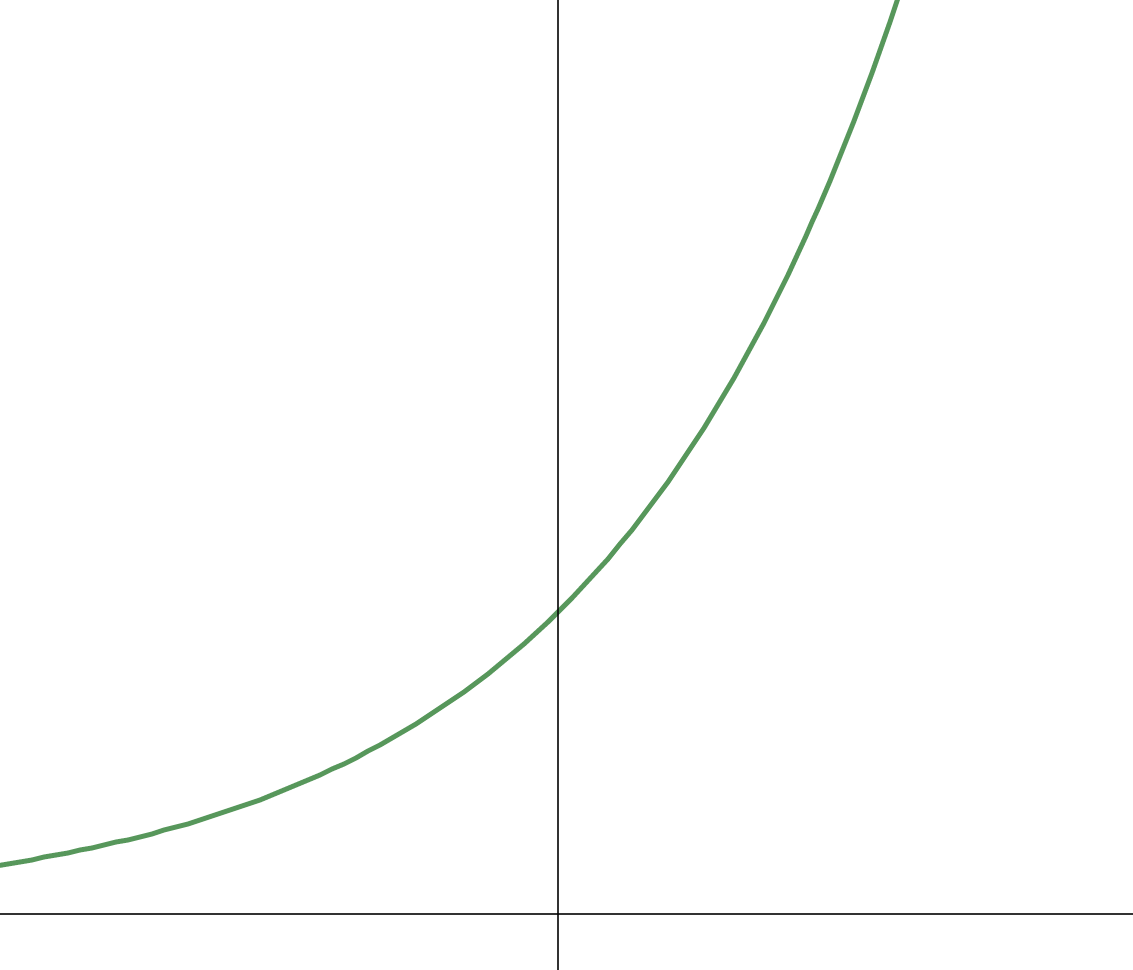
\includegraphics[width=0.8\textwidth, angle=0]{Grafico2.png}
\end{center}
\caption{$f'(x)>0, \forall x\in I$.}
\end{figure}

\begin{figure}[htbp]
\begin{center}
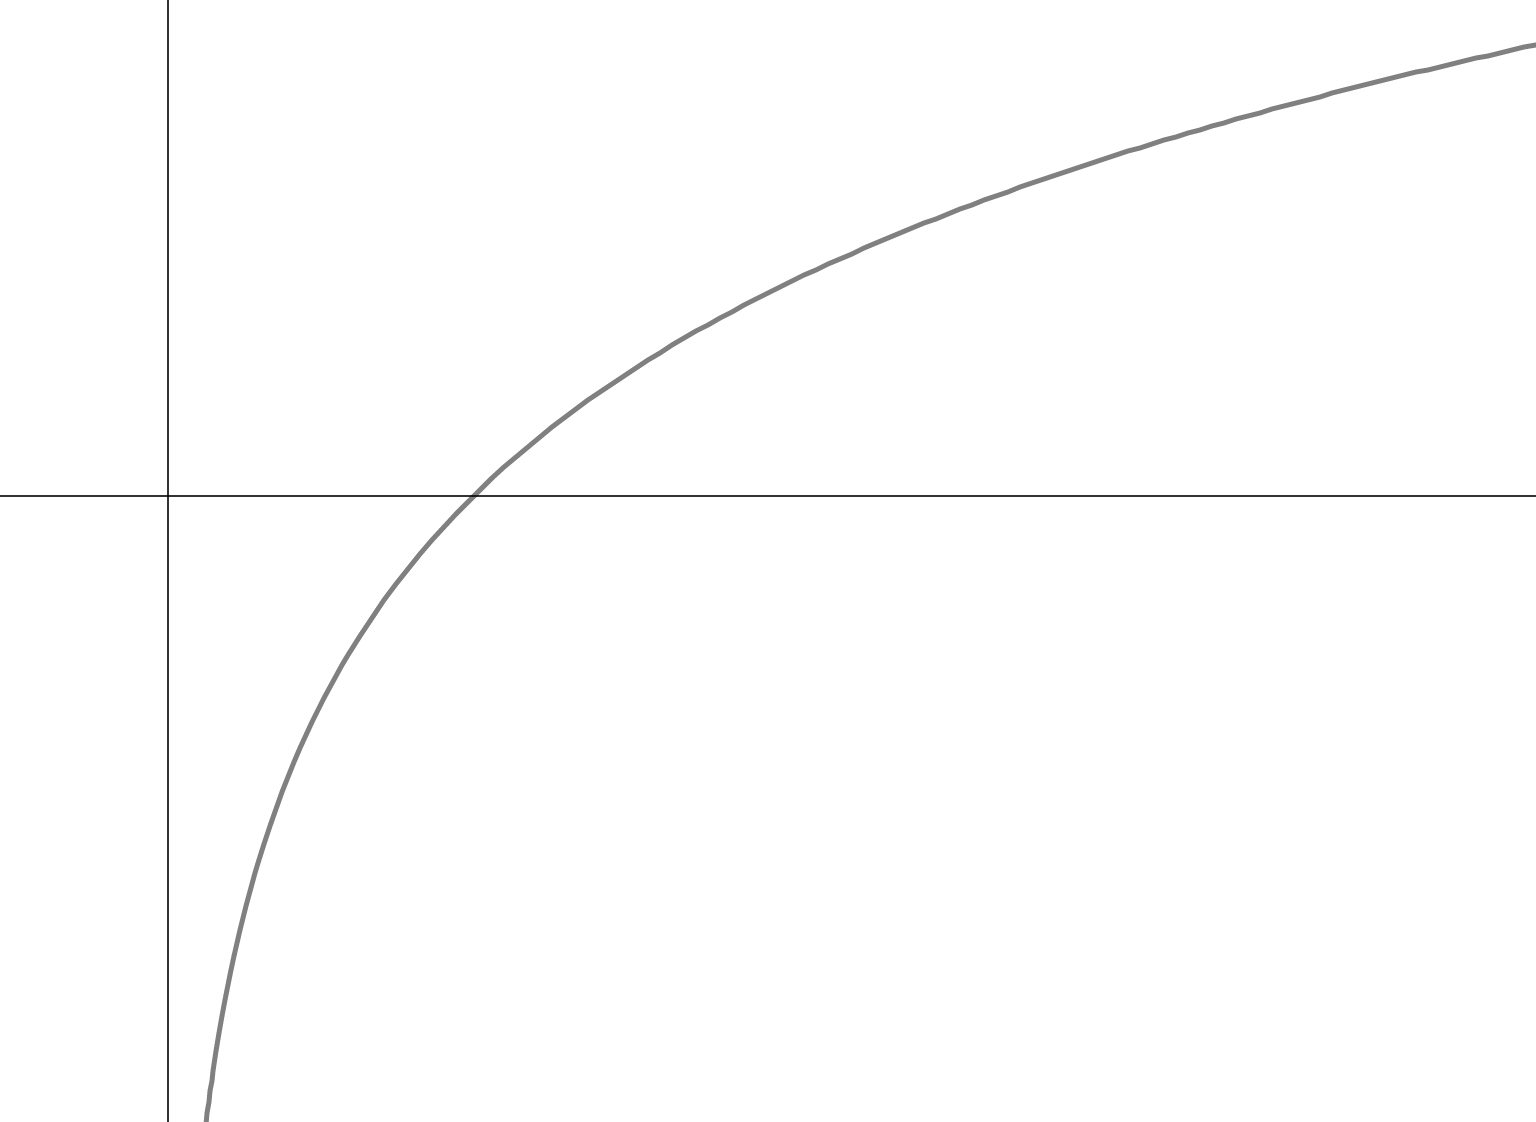
\includegraphics[width=0.6\textwidth, angle=0]{Grafico3.png}
\end{center}
\caption{$f'(x)>0, \forall x\in I$.}
\end{figure}

\begin{figure}[htbp]
\begin{center}
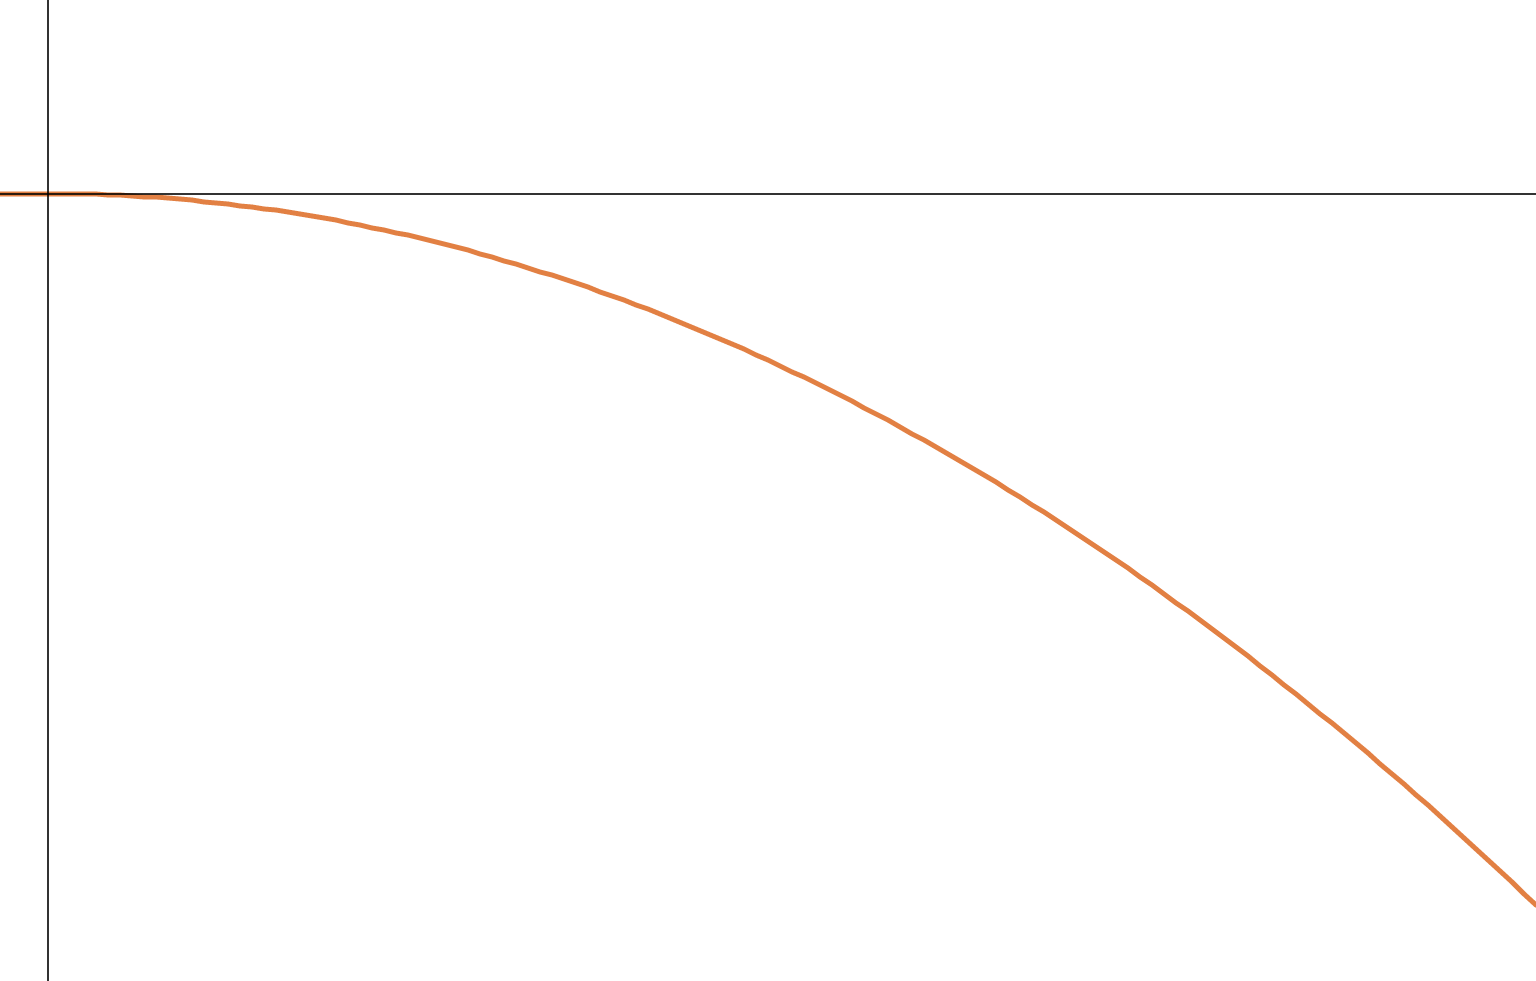
\includegraphics[width=0.6\textwidth, angle=0]{Grafico4.png}
\end{center}
\caption{$f'(x)<0, \forall x\in I$.}
\end{figure}

%\begin{figure}[htbp]
%\begin{center}
%\includegraphics[width=0.6\textwidth, angle=0]{Grafico5.png}
%\end{center}
%\caption{$f'(x)<0, \forall x\in I$.}
%\end{figure}

\begin{newpage}
\vspace{0.3cm}
\par Note que a reta tangente ao gráfico de uma função $y=f(x)$ em um ponto $(p;f(p))$ é dada por:
\begin{equation*} y - f(p) = f'(p)\cdot (x - p) \Rightarrow y = f(p) + f'(p)\cdot (x - p) .\end{equation*}
\par Então, podemos definir a função
\begin{equation*} T(x) = f'(p)\cdot (x - p) + f(p), \forall x\in I, p\in I .\end{equation*}
\end{newpage}
\vspace{0.3cm}
\begin{flushleft}
\textbf{Definição 1}
\end{flushleft}
\hspace{12pt} Uma função $y=f(x)$ tem concavidade para cima em um intervalo $I$ se para quaisquer $x,p\in I, x\neq p$, tivermos:
\begin{equation*} T(x)<f(x) \Leftrightarrow f(x) - T(x)>0, \forall x,p\in I, x\neq p .\end{equation*}
  
\begin{figure}[htbp]
\begin{center}
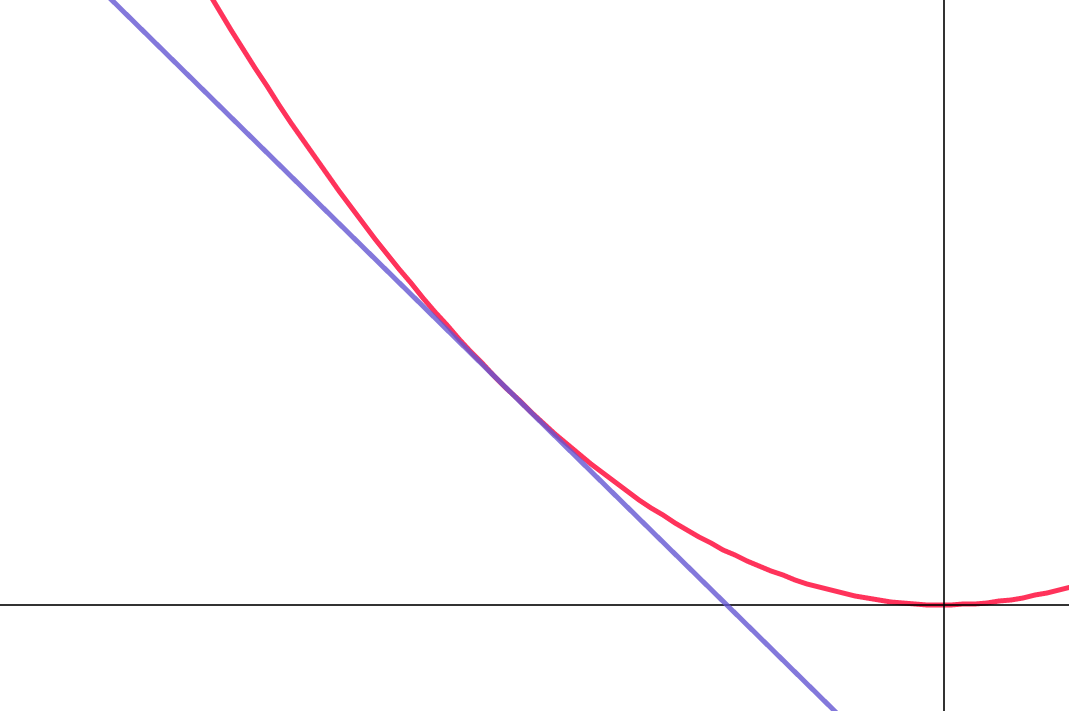
\includegraphics[width=0.5\textwidth, angle=0]{Grafico6.png}
\end{center}
\caption{a reta azul representa $T(x)$.}
\end{figure}

\par
\vspace{0.3cm}
\begin{flushleft}
\textbf{Definição 2}
\end{flushleft}
\hspace{12pt} Uma função $y=f(x)$ tem concavidade para baixo em $I$ se para quaisquer $x,p\in I, x\neq p$, tivermos:
\begin{equation*} T(x) > f(x) \Leftrightarrow T(x) - f(x)>0, \forall x,p \in I, x\neq p. \end{equation*}

\begin{figure}[htbp]
\begin{center}
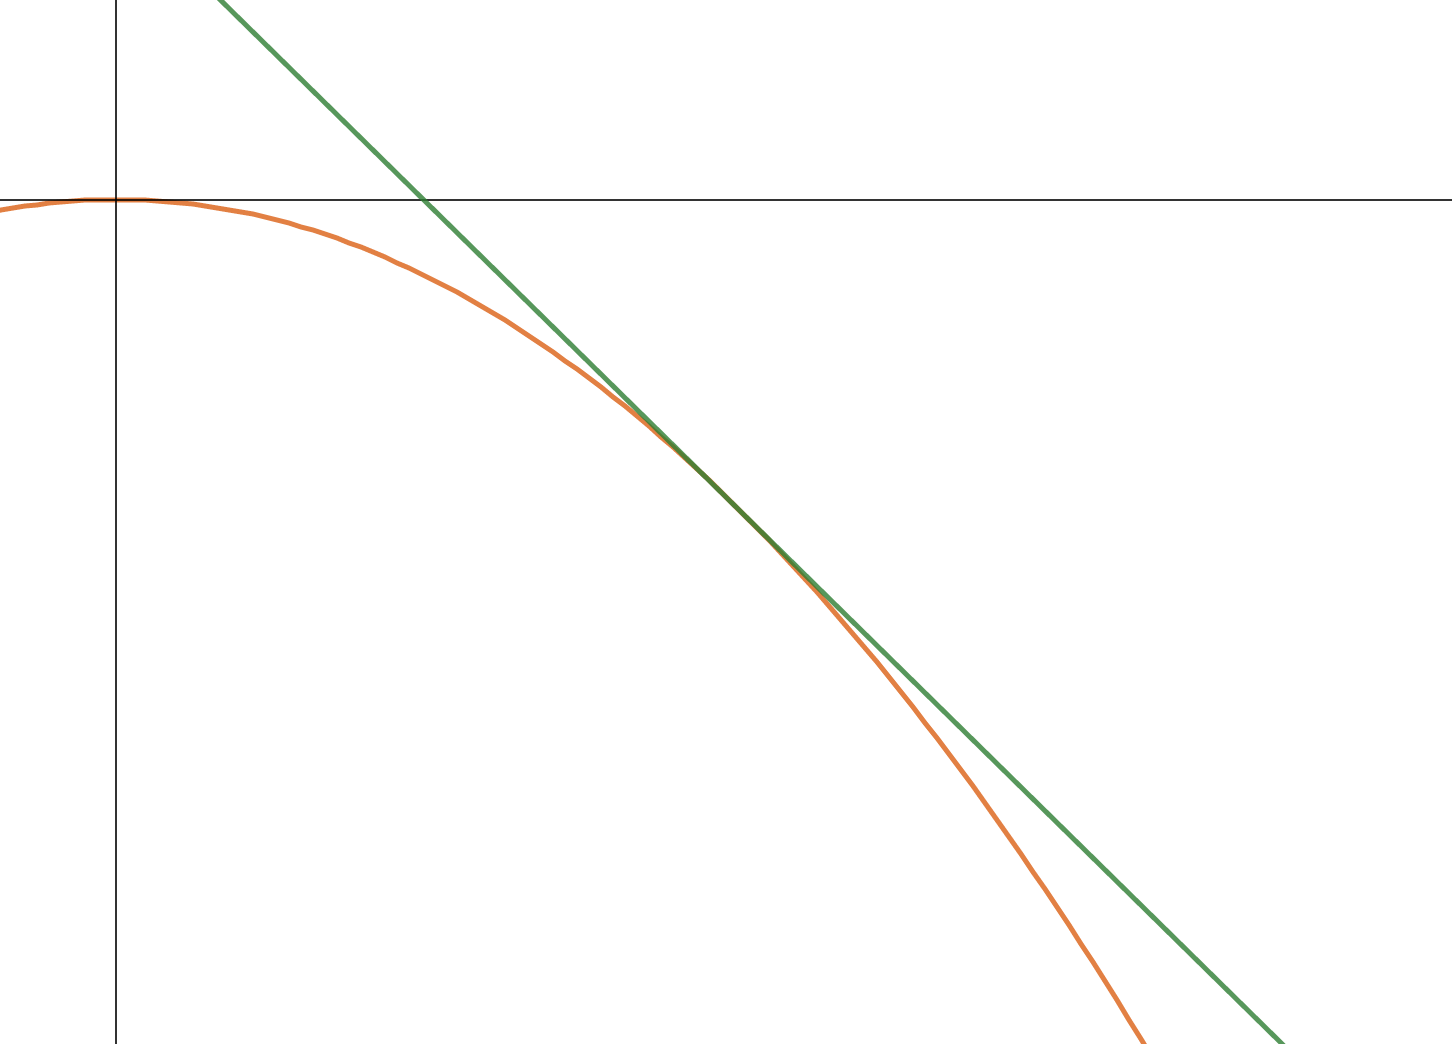
\includegraphics[width=0.5\textwidth, angle=0]{Grafico7.png}
\end{center}
\caption{a reta verde representa $T(x)$.}
\end{figure}

\par
\vspace{0.3cm}
\textbf{Teorema}
\par Seja $y=f(x)$ uma função derivável, pelo menos, duas vezes. É possível provar que:
\begin{itemize}
\item a) Se $f''(x)>0, \forall x\in I$, então $f$ tem concavidade para cima em $I$;
\item b) Se $f''(x)<0, \forall x\in I$, então $f$ tem concavidade para baixo em $I$.
\end{itemize}
\par
\vspace{0.3cm}
\begin{flushleft}
\textbf{Definição 3}
\end{flushleft}
\par Um ponto $p$ do domínio de uma função $y=f(x)$ é dito ponto crítico se $f'(p)=0$ ou se não existe $f'(p)$.
\par
\vspace{0.3cm}
\begin{flushleft}
\textbf{Definição 4}
\end{flushleft}
\par Um ponto $p$ do domínio de uma função $y=f(x)$ é dito ponto de inflexão se $f$ tiver concavidades de nomes diferentes nos intervalos $]a,p[$ e $]p,b[$.
\par
\vspace{0.3cm}
\textbf{Teorema}
\par Se $y=f(x)$ é uma função derivável, pelo menos, duas vezes, em um intervalo $I$ com $p\in I$, então valem as afirmativas:
\begin{itemize}
\item a) Se $p$ é um ponto crítico de $y=f(x)$ e $f'(p)$ existe, então $f'(p)=0$;
\item b) Se $p$ é um ponto de inflexão de $y=f(x)$ e $f''(p)$ existe, então $f''(p)=0$;
\item c) Se $f'(p) = 0$ e $f''(p)>0$, então $x=p$ é um ponto de mínimo:
\par
\hspace{12pt} (i) local ou relativo se $f(x)\geq f(p), \forall x\in I, p\in I$;
\par
\hspace{12pt} (ii) absoluto se $f(x)\geq f(p), \forall x\in D(f), p\in D(f)$;
\item Se $f'(p)=0$ e $f''(p)<0$, então $x=p$ é um ponto de máximo:
\par
\hspace{12pt} local ou relativo se $f(x)\leq f(p), \forall x\in I, p\in I$;
\par
\hspace{12pt} absoluto se $f(x)\leq f(p), \forall x\in D(f), p\in D(f)$.
\end{itemize}
\par
\vspace{0.3cm}
\subsection{Exercícios - intervalos de crescimento e de decrescimento}
\vspace{0.3cm}
\begin{flushleft}
1. Determine os intervalos de crescimento e de decrescimento de $f(x)$ e, em seguida, faça um esboço de $f$, sendo:
\end{flushleft}
\par
\begin{multicols}{2}
\hspace{-15pt}a)$f(x) = x^3 - 2x^2 + x + 2$\\
b)$f(x)=\displaystyle{\frac{x^2 - x}{1 + 3x^2}}$\\
c)$f(x)=\displaystyle{\frac{x^2}{x^2 - 1}}$\\
d)$f(x)=x\cdot e^{-2x}$\\
e)$f(x)=\displaystyle{\frac{\ln{x}}{x}}$\\
\end{multicols}
\par
\vspace{0.3cm}
\subsection{Taxas relacionadas e problemas de máximo e mínimo}
\hspace{12pt} Se uma quantidade $x$ é uma função do tempo $t$, então a taxa de variação de $x$ com relação ao tempo $t$ é definida por $\displaystyle{\frac{dx}{dt}}$.
\par
\vspace{0.3cm}
Exemplos.
\par
\begin{flushleft}
1. O gás de um balão esférico está escapando a uma taxa de $2m^{3}/min$. A que taxa a superfície do balão está encolhendo quando o raio é $12m$? 
\end{flushleft}
\vspace{0.3cm}
\begin{flushleft}
1.1 Resolução.
\end{flushleft}
\par Note que $\displaystyle{\frac{dV}{dt} = 2m^{3}/min}$ e que o raio $R$ do balão é uma função do tempo, $R(t)$. Dado que o volume de uma esfera de raio $R$ é $\displaystyle{\frac{4\pi R^3}{3}}$, temos:
\begin{equation*} \displaystyle{\frac{dV}{dt} = \frac{4\pi }{3}\cdot 3R^{2}\cdot\frac{dR}{dt} \Rightarrow -2 = 4\pi R^{2}\cdot\frac{dR}{dt} \Rightarrow \frac{dR}{dt} = -\frac{1}{2\pi R^2}}. \end{equation*}
\par Sendo a área da superfície de uma esfera $S=4\pi R^{2}$, temos:
\begin{equation*} \displaystyle{\frac{dS}{dt} = 4\pi\cdot 2R\cdot\frac{dR}{dt} \Rightarrow \frac{dS}{dt} = -\frac{8\pi R}{2\pi R^2} \Rightarrow \frac{dS}{dt} = -\frac{4}{R}}. \end{equation*}
\par Para $R=12m$, temos:
$$\displaystyle{\frac{dS}{dt} = -\frac{1}{3}m^{3}/min}.$$
\par Os sinais de $-$ indicam apenas que tanto o volume quanto a área são funções decrescentes de $t$.
\par
\vspace{0.3cm}
\begin{flushleft}
2. Uma escada de $6m$ de comprimento está apoiada em uma parede vertical. Se a base da escada começar a deslizar horizontalmente, à razão de $0,6m/s$, com que velocidade o topo da escada percorre a parede, quando está a $4m$ do solo?
\end{flushleft}
\vspace{0.3cm}
\begin{flushleft}
2.1 Resolução.
\end{flushleft} 
\par Observe a figura:

\begin{figure}[htbp]
\begin{center}
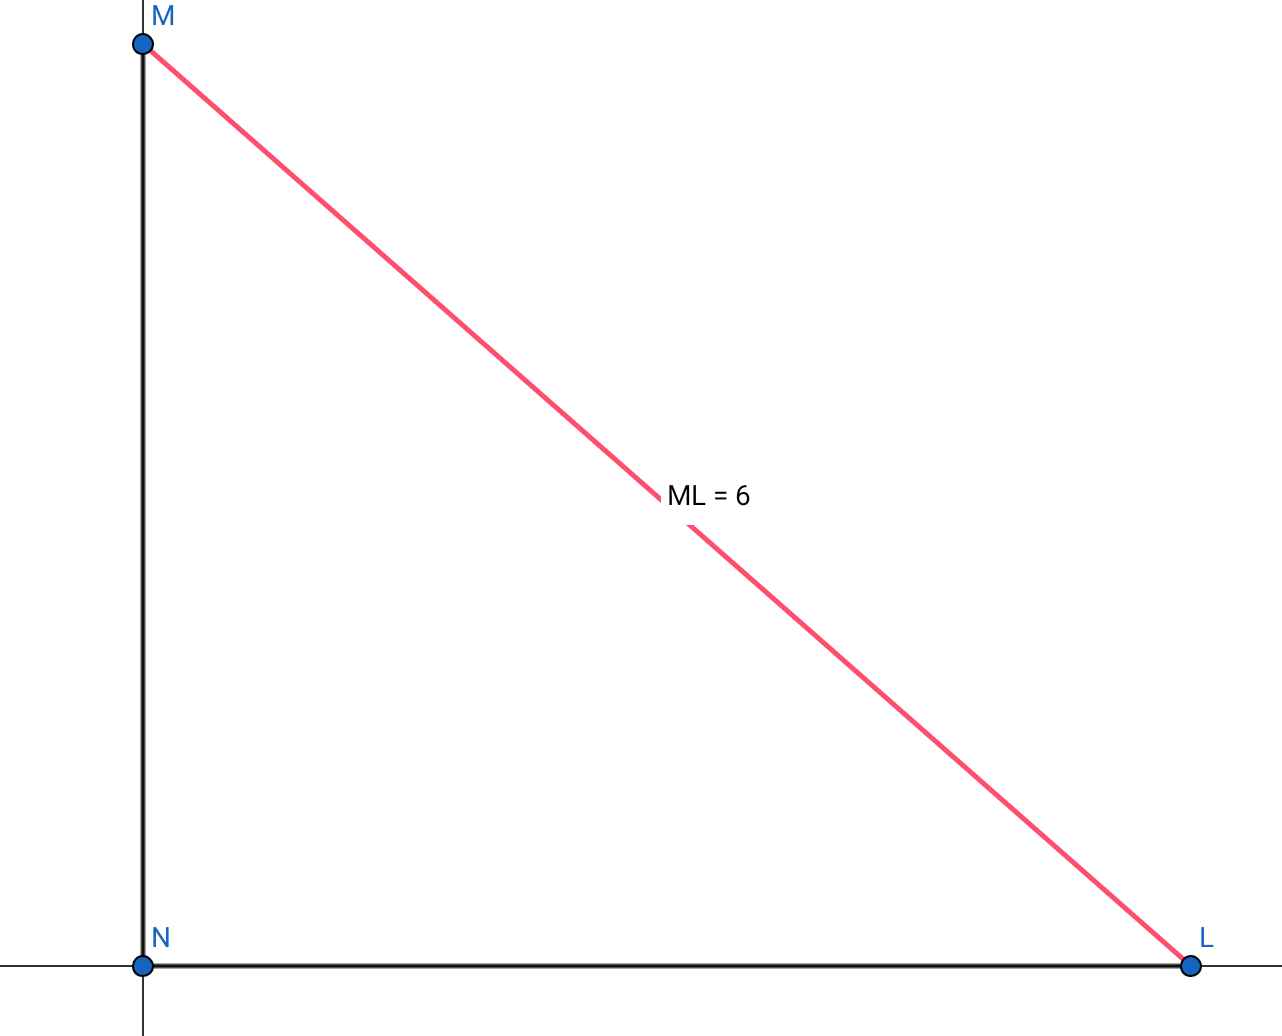
\includegraphics[width=0.5\textwidth, angle=0]{Escada.png}
\end{center}
\caption{O triângulo é retângulo em N e os segmentos MN e NL medem, respectivamente, $y$ e $x$ metros.}
\end{figure}
\par Note que tanto $y$ quanto $x$ são funções do tempo, $y(t)$ e $x(t)$, e que $\displaystyle{\frac{dx}{dt} = 0,6m/s}$. Além disso, como $\triangle MNL$ é retângulo, $x^2 + y^2 = 36$. Derivando ambos os membros da igualdade em relação $t$, obtemos:
\begin{equation*} \displaystyle{0 = 2x\cdot\frac{dx}{dt} + 2y\cdot\frac{dy}{dt} \Rightarrow \frac{dy}{dt} = -\frac{x}{y}\cdot\frac{6}{10}}. \end{equation*}
\par Queremos descobrir o valor de $\displaystyle{\frac{dy}{dt}}$ para $y=4m$. Perceba que, se $y=4m$, então $x=\sqrt{36-16} = 2\sqrt{5}m$, $x>0$. Substituindo os valores em $\displaystyle{\frac{dy}{dt}}$, tem-se:
$$\displaystyle{\frac{dy}{dt} = -\frac{3\sqrt{5}}{10}m/s}$$
\par O sinal de $-$ indica que a escada está descendo.
\par
\vspace{0.3cm}
\begin{flushleft}
3. A areia caindo de uma calha forma um monte em forma de cone cuja altura é sempre igual a $\displaystyle{\frac{4}{3}}$ do raio da base.\\
\hspace{12pt}a) A que taxa está aumentando o volume quando o raio da base é $3m$ e está crescendo a uma taxa de $25cm/min$?\\
\hspace{12pt}b) A que taxa está crescendo o raio da base desse cone quando o seu comprimento é $6m$ e o volume está aumentando à taxa de $24m^{3}/min$?
\end{flushleft}
\par
\vspace{0.3cm}
\begin{flushleft}
3.1 Resolução.
\end{flushleft}
\par a) Do enunciado, a altura $H$ do cone é $\displaystyle{\frac{4R}{3}}$, em que $R=R(t)$ é o raio da base. Como o volume do cone é $\displaystyle{\frac{\pi R^{2}H}{3} = \frac{4\pi R^{3}}{9}}$, obtemos a seguinte relação:
\begin{equation*} \displaystyle{\frac{dV}{dt} = \frac{4\pi 3R^{2}}{9}\cdot\frac{dR}{dt} \Rightarrow \frac{dV}{dt} = \frac{4\pi R^2}{3}\cdot\frac{dR}{dt}}. \end{equation*}
\par Dado que $R = 3m$ e $\displaystyle{\frac{dR}{dt} = 25\cdot 10^{-2}m/min}$, temos:
\begin{equation*} \displaystyle{\frac{dV}{dt} = \frac{4\pi\cdot 9}{3}\cdot 25\cdot 10^{-2} \Rightarrow \frac{dV}{dt} = 3\pi m^{3}/min}.\end{equation*}
\vspace{0.2cm}
\par b) Do enunciado, $R=6m$ e $\displaystyle{\frac{dV}{dt} = 24m^{3}/min}.$ Substituindo os dados em $\displaystyle{\frac{dV}{dt} = \frac{4\pi R^2}{3}\cdot\frac{dR}{dt}}$, obtém-se:
\begin{equation*}\displaystyle{24 = \frac{4\pi\cdot 3\cdot 36}{9}\cdot\frac{dR}{dt} \Rightarrow \frac{dR}{dt} = \frac{1}{2\pi }m/min}.\end{equation*}
\par
\vspace{0.3cm}
\begin{flushleft}
4. Um tanque tem a forma de um cone circular reto invertido, com $H=4m$ de altura e $R=2m$ de raio da base. Se a água entra no tanque à razão de $0.001m^{3}/min$, calcule aproximadamente a razão no qual o nível da água está subindo quando a profundidade é de $1m$. 
\end{flushleft}
\par
\vspace{0.3cm}
\begin{flushleft}
4.1 Resolução.
\end{flushleft}
\par Seja $h=h(t)$ a altura da água no instante $t$ e $r$ o raio do cone de água correspondente. Por semelhança $\displaystyle{\frac{R}{H} = \frac{r}{h} \Rightarrow r=\frac{h}{2}}.$ Dado que o volume do cone de água é igual a $\displaystyle{V = \frac{\pi r^{2}h}{3} \Rightarrow V=\frac{\pi\cdot h^3}{12}}$, temos:
\begin{equation*}\displaystyle{\frac{dV}{dt} = \frac{3\pi\cdot h^2}{12}\cdot\frac{dh}{dt} \Rightarrow \frac{dh}{dt} = \frac{dV}{dt}\cdot\frac{4}{\pi\cdot h^2}}.\end{equation*}
\par Substituindo $h=1m$ e $\displaystyle{\frac{dV}{dt} = 10^{-3}m^{3}/min}$, segue:
\begin{equation*}\displaystyle{\frac{dh}{dt} = \frac{4\cdot 10^{-3}}{\pi } = \frac{0,004}{\pi }m/min \approx 0,00127 m/min}.\end{equation*}
\par
\vspace{0.3cm}
\begin{flushleft}
5. A área de um triângulo equilátero decresce à razão de $4cm^{2}/min$. Determine a taxa na qual o comprimento do lado está variando quando a área do triângulo é $200cm^{2}$.
\end{flushleft}
\par
\vspace{0.3cm}
\begin{flushleft}
5.1 Resolução.
\end{flushleft}
\par Seja $l=l(t)$ o comprimento do lado do triângulo. É possível mostrar que a área $S$ de um triângulo equilátero de lado $l$ vale $S=\displaystyle{\frac{l^{2}\sqrt{3}}{4}}$. Daí, temos:
\begin{equation*} \displaystyle{\frac{dS}{dt} = \frac{l\sqrt{3}}{2}\cdot\frac{dl}{dt} \Rightarrow -4 = \frac{l\sqrt{3}}{2}\cdot\frac{dl}{dt}\Rightarrow \frac{dl}{dt} = -\frac{8}{l\sqrt{3}}}.\end{equation*}
\par Note que, se $S=200cm^{2}$, $l=\displaystyle{\frac{20\sqrt{2}\sqrt[4]{3}}{\sqrt{3}}}$, $l>0$. Substituindo $S$ e $l$, tem-se:
\begin{equation*}\displaystyle{\frac{dl}{dt} = -\frac{8}{20\sqrt{2}\cdot\sqrt[4]{3}} \Rightarrow \frac{dl}{dt} = -\frac{\sqrt{2}}{5\cdot\sqrt[4]{3}}cm/min}.\end{equation*}
\par
\vspace{0.3cm}
\section{Integral definida}
\subsection{Integrais definidas a partir de somas de Riemann}
\hspace{12pt}
\textbf{Definição (integral definida)}: seja $y=f(x)$ uma função definida no intervalo $[a;b]$, com $f(x)\geq 0, \forall x\in [a;b]$. Seja $x_0 = a < x_1 < x_2 < \cdots < x_n = b$ uma partição de $[a;b]$ e $\xi _i$ um ponto qualquer do subintervalo $[x_{i-1} ;x_i ], \forall i=1,2,...,n$. O limite $\displaystyle{\lim_{n\to \infty } \sum_{i=1}^{n} f(\xi _i)\cdot\Delta x}$, quando existe, é indicado por $\displaystyle{\int_{a}^{b} f(x)\, dx}$ e é chamado integral definida em $[a;b]$, sendo $a$ o limite inferior e $b$ o limite superior. 
\par
\vspace{0.3cm}
Exemplos.
\par
\vspace{0.3cm}
\begin{flushleft}
1. Calcule a área da região delimitada pela curva $y=x^2$, o eixo $x$ e a reta $x=3$, tomando retângulos inscritos.
\end{flushleft}
\par
\vspace{0.3cm}
\begin{flushleft}
1.1 Resolução.
\end{flushleft}
\par Observe a figura.
\begin{figure}[htbp]
\begin{center}
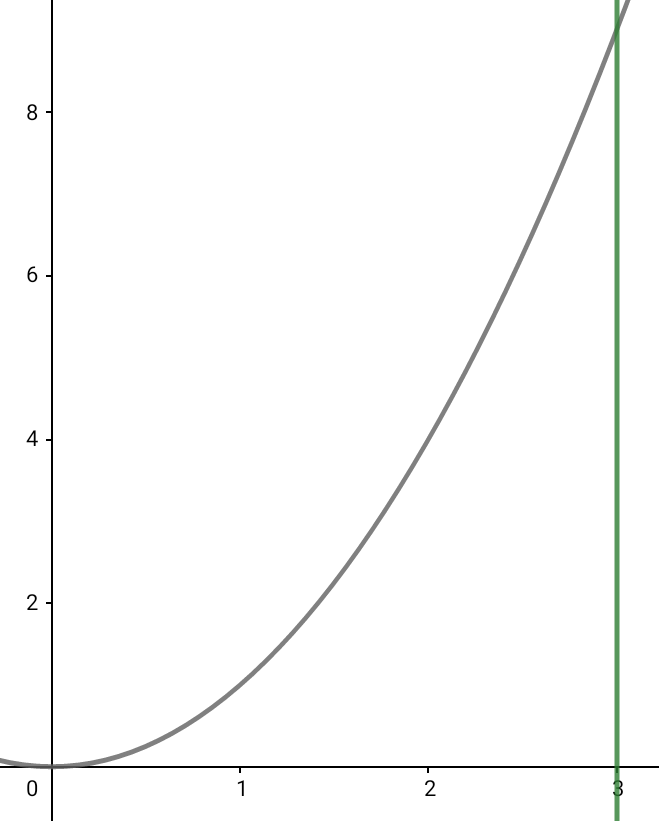
\includegraphics[width=0.5\textwidth, angle=0]{Grafico8.png}
\end{center}
\end{figure}
\par Inicialmente, vamos dividir o intervalo $[0;3]$ em $n$ subintervalos, todos com o mesmo comprimento. Para isso, consideremos os pontos $0 = x_0 < x_1 < x_2 < \cdots < x_n = b$, com o comprimento $\displaystyle{\Delta x = x_i - x_{i-1} = \frac{3-0}{n} = \frac{3}{n}, \forall i=1,...,n.}$
\par Observe que $x_0 = 0$, $x_1 = \Delta x = \displaystyle{\frac{3}{n}}$, ... ,$x_{i-1} = (i-1)\cdot\Delta x = \displaystyle{(i-1)\cdot\frac{3}{n}}$, ... ,$x_n = n\cdot\Delta x = 3$.
\par A área da região limitada pela curva $y=x^2$, pelo eixo $x$ e a reta $x=3$ é definida por:
\begin{equation*} \displaystyle{\begin{split} &\lim_{n\to \infty } \sum_{i=1}^{n} f(x_{i-1})\cdot\Delta x = \lim_{n\to \infty } \sum_{i=1}^{n} \frac{3}{n}\cdot x^{2}_{i-1} = \lim_{n\to \infty } \frac{3}{n}\cdot\sum_{i=1}^{n} \Big( (i-1)\cdot\frac{3}{n} \Big)^{2} = \\ =&\lim_{n\to \infty } \frac{27}{n^3}\cdot\sum_{i=1}^{n} (i-1)^{2} = \lim_{n\to \infty } \frac{27}{n^3}\cdot\Big( \sum_{i=1}^{n} i^2 - 2\sum_{i=1}^{n} i + \sum_{i=1}^{n} 1 \Big) .  \end{split}} \end{equation*}
\par
\vspace{0.2cm}
\par Com um pouco de álgebra, vemos que:
\begin{equation*} \sum_{i=1}^{n} 1 = n. \end{equation*}
\begin{equation*} \sum_{i=1}^{n} i = \frac{n(n+1)}{2}. \end{equation*}
\begin{equation*} \sum_{i=1}^{n} i^{2} = \frac{n(n+1)(2n+1)}{6}. \end{equation*}
\par Logo, temos:
\begin{equation*}\displaystyle{\begin{split} &\lim_{n\to \infty } \frac{27}{n^3}\cdot\Big( \sum_{i=1}^{n} i^2 - 2\sum_{i=1}^{n} i + \sum_{i=1}^{n} 1           \Big) = \lim_{n\to \infty }\frac{27}{n^3}\cdot\Big( \frac{n(n+1)(2n+1)}{6} - n(n+1) + n \Big) = \\ =& \lim_{n\to \infty } \frac{27}{n^2}\cdot\Big( \frac{(n+1)(2n+1)}{6} - n \Big) = \frac{27}{6}\cdot\lim_{n\to \infty } \frac{2n^2 - 3n + 1}{n^2} = \frac{9}{2}\cdot\lim_{n\to \infty } 2 - \frac{3}{n} + \frac{1}{n^2} = 9u.a.  \end{split}} \end{equation*} 
\par Note que, utilizando a definição, acabamos de provar que $\displaystyle{\int_{0}^{3} x^{2}\, dx}=9$.
\par
\vspace{0.3cm}
\begin{flushleft}
2. Calcule a área do trapézio limitado pelas retas $x=1$ e $x=3$, pelo eixo $x$ e pela reta $2x + y = 8$.
\end{flushleft}
\par
\vspace{0.3cm}
\begin{flushleft}
2.1 Resolução.
\end{flushleft}
\par Observe o gráfico.
\begin{figure}[htbp]
\begin{center}
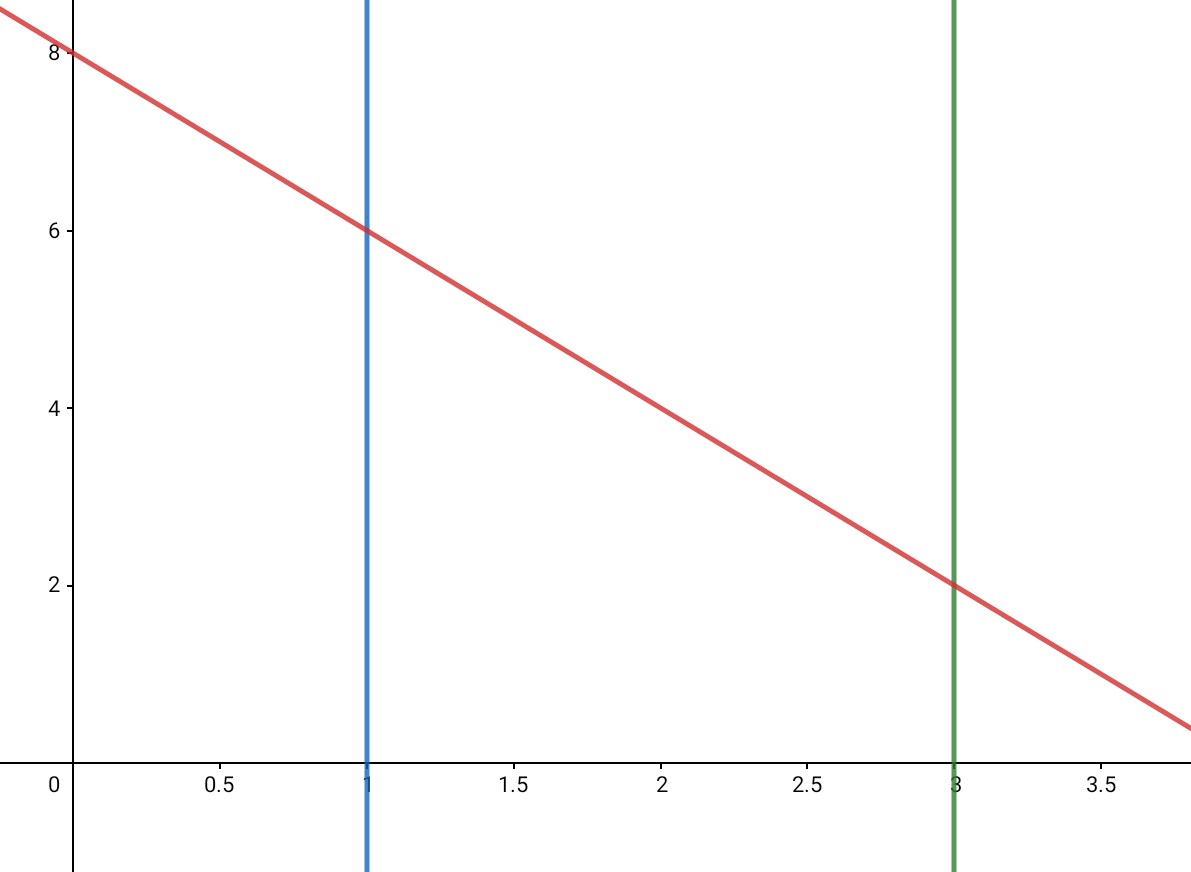
\includegraphics[width=0.6\textwidth, angle=0]{Grafico9.png}
\end{center}
\caption{a reta vermelha representa $y=-2x + 8$.}
\end{figure}
\par Consideremos uma partição $x_0 = 1 < x_1 < x_2 < ... < x_{i-1} < x_i < ... < x_n = 3$, com $\Delta x = x_i - x_{i-1} = \displaystyle{\frac{2}{n}}, \forall i=1,2,...,n.$
\par A área do trapézio da figura acima é dada por:
\begin{equation*}\displaystyle{\begin{split} &\lim_{n\to \infty } \sum_{i=1}^{n} f(x_i)\cdot\Delta x = \lim_{n\to \infty } \sum_{i=1}^{n} f\Big(1 + \frac{2i}{n}\Big)\cdot\Delta x = \lim_{n\to \infty } \frac{2}{n}\cdot\sum_{i=1}^{n} -2\Big( 1 + \frac{2i}{n} \Big) + 8 = \lim_{n\to \infty } \frac{2}{n}\cdot\sum_{i=1}^{n} 6 - \frac{4i}{n} = \\ = &\lim_{n\to \infty } \frac{2}{n}\Big( 6n - \frac{4}{n}\cdot\sum_{i=1}^{n} i \Big) = \lim_{n\to \infty } \frac{2}{n}\cdot\Big( 6n - \frac{4}{n}\cdot\frac{n(n+1)}{2} \Big) = \lim_{n\to \infty } 12 - \frac{4(n+1)}{n} = 8u.a.\end{split}}\end{equation*}
\par Acabamos de verificar que $\displaystyle{\int_{1}^{3} (-2x + 8)\, dx = 8}$.
\par
\subsection{1° Teorema Fundamental do Cálculo}
\hspace{12pt} Se $F(x)$ é uma primitiva de $f(x)$ em $[a;b]$, $f(x)$ contínua em $[a;b]$,  isto é, $F'(x) = f(x)$ em $[a;b]$, então $\displaystyle{\int_{a}^{b} f(x)\, dx = F(x) \Big|^{b}_{a} = F(b) - F(a) .}$
\par
\vspace{0.3cm}
\textbf{Observação 1}. Se $f(x)\geq 0, \forall x\in [a;b]$, com primitiva $F(x)$, então a integral definida $\displaystyle{\int_{a}^{b} f(x)\, dx}$ nos dá a área delimitada pelas retas $x=a, x=b$, pelo eixo $x$ e pelo gráfico de $f$.
\begin{figure}[htbp]
\begin{center}
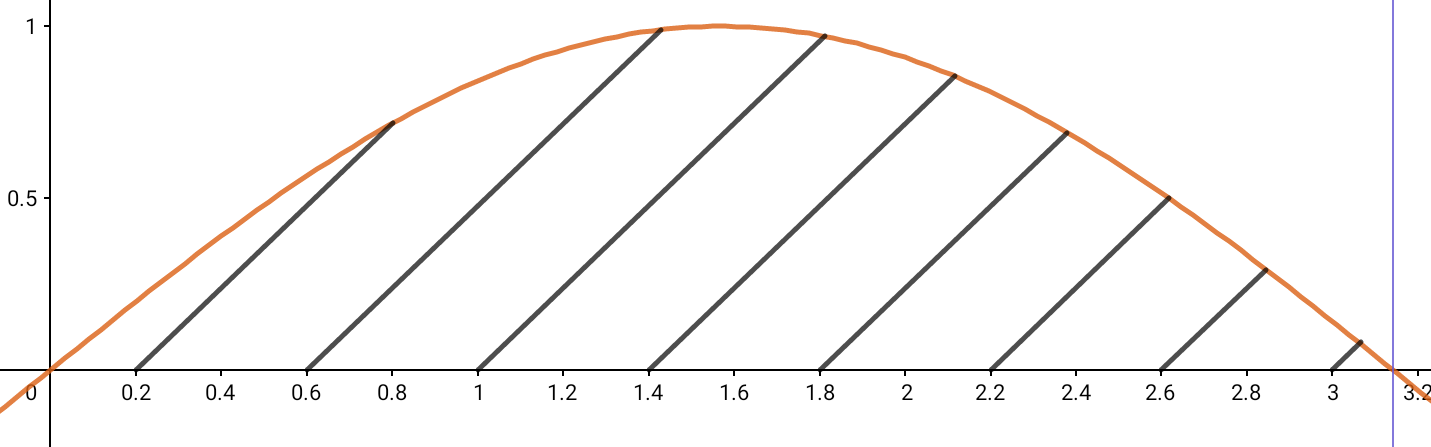
\includegraphics[width=0.5\textwidth, angle=0]{Grafico10.png}
\end{center}
\caption{$\displaystyle{\int_{a}^{b} f(x)\, dx = F(b) - F(a)}$.}
\end{figure}  
\par
\vspace{0.3cm}
\textbf{Observação 2}. Observe a figura 9.
\begin{figure}[htbp]
\begin{center}
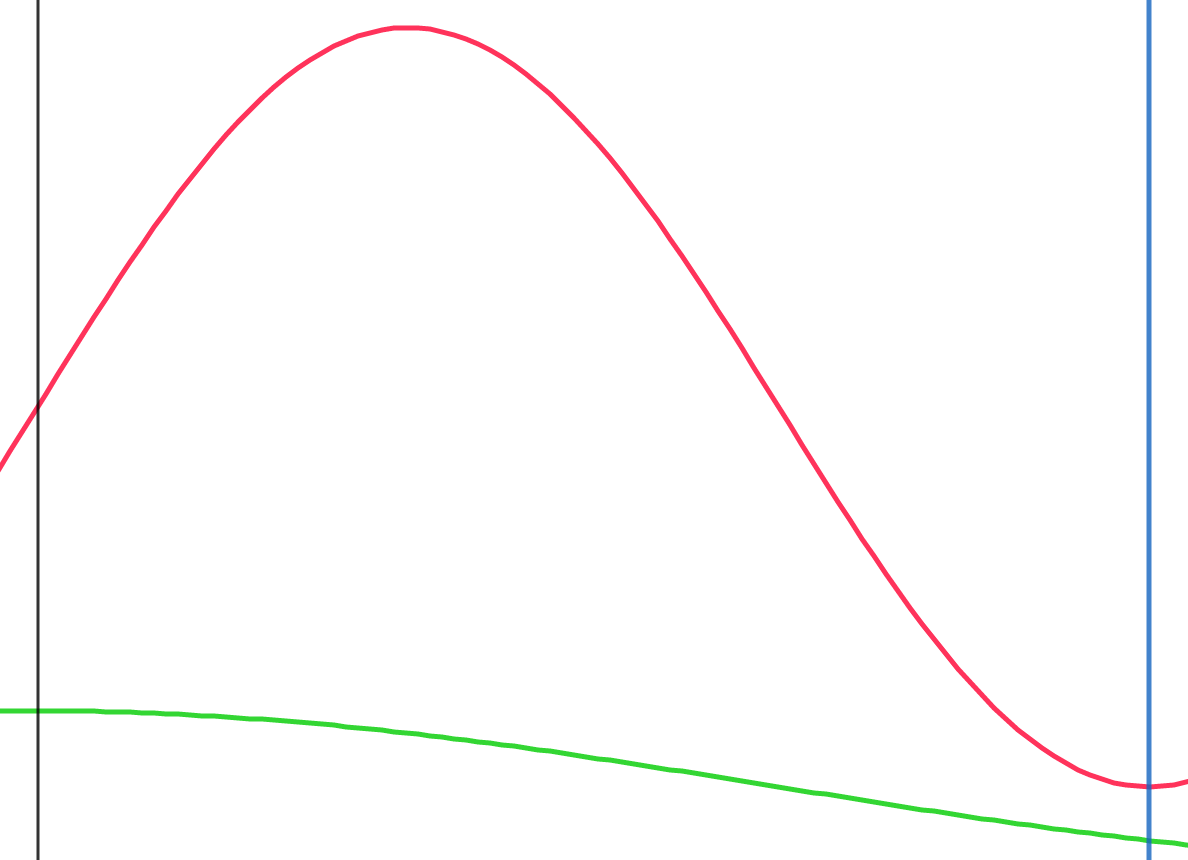
\includegraphics[width=0.5\textwidth, angle=0]{Grafico11.png}
\end{center}
\caption{a área entre a função vermelha ($y=f(x)$), a função verde ($y=g(x)$), a reta preta ($x=a$) e a reta azul ($x=b$) é dada pela integral definida: $\displaystyle{\int_{a}^{b} (f(x) - g(x))\, dx}$. }
\end{figure}
\par
\vspace{0.3cm}
\textbf{Obervação 3}. Considere a figura 10.
\begin{figure}[htbp]
\begin{center}
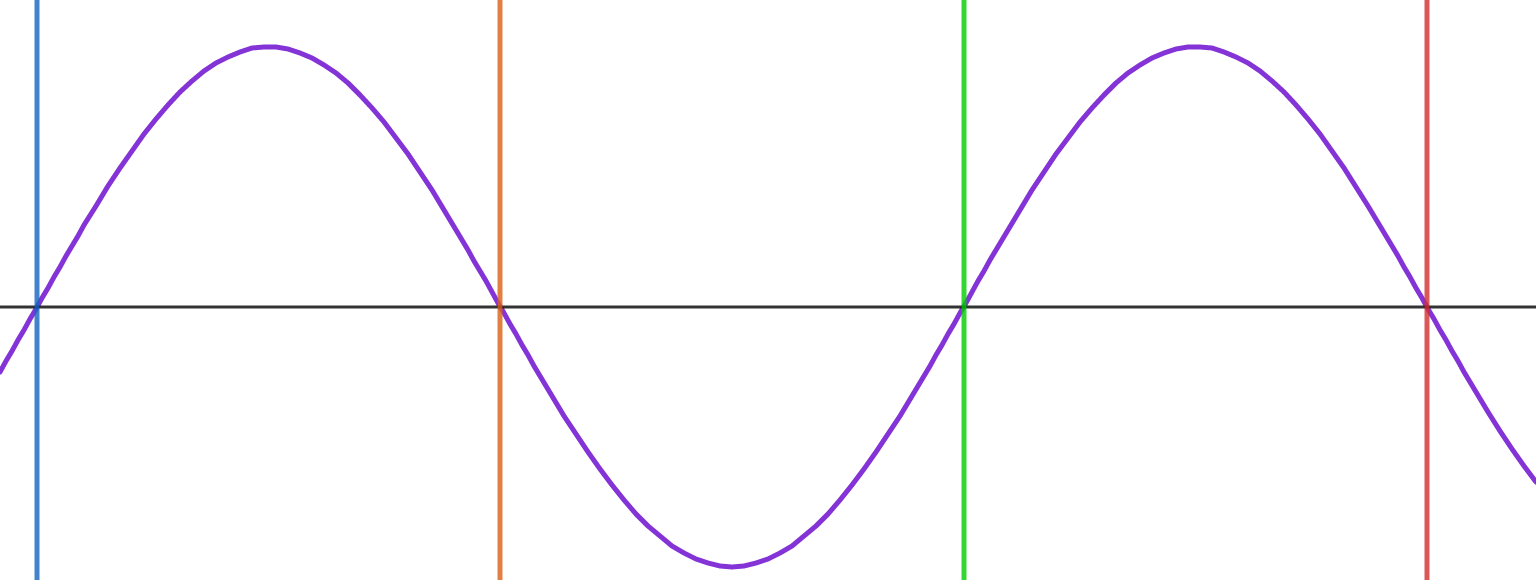
\includegraphics[width=0.5\textwidth, angle=0]{Grafico12.png}
\end{center}
\caption{a área entre a função roxa ($y=f(x)$) e as retas azul ($x=a$), laranja ($x=b$), verde ($x=c$), vermelha ($x=d$) e preta (eixo $x$)  é dada pela integral definida: $\displaystyle{\int_{a}^{b} f(x)\, dx - \int_{b}^{c} f(x)\, dx  + \int_{c}^{d} f(x)\, dx }$. }
\end{figure}
\par
\vspace{0.3cm}
Exemplos.
\par
\begin{flushleft}
1. Calcule a área delimitada por $f(x)=\displaystyle{\frac{1}{x}}$, o eixo $x$ e as retas $x=-5$ e $x=-1$.
\end{flushleft}
\par
\vspace{0.3cm}
\begin{flushleft}
1.1 Resolução.
\end{flushleft}
\par Note que $f(x)=\displaystyle{\frac{1}{x}}$ é contínua em $[-5;-1]$.Portanto, podemos escrever que a área desejada é igual a:

\begin{equation*} \displaystyle{-\int_{-5}^{-1} \frac{dx}{x} = -\ln{|x|}\Big|^{-1}_{-5} = -(\ln{|-1|} - \ln{|-5|}) = \ln{5}}. \end{equation*}
\par Perceba também que não podemos utilizar o Teorema Fundamental do Cálculo para calcular $\displaystyle{\int_{-1}^{1} \frac{1}{x}}$, já que $f(x) = \displaystyle{\frac{1}{x}}$ é descontínua em 0. 
\par
\vspace{0.3cm}
\begin{flushleft}
2. Calcular a área da região determinada pelas retas $y=3-2x$ e pela parábola $y=x^2$ no intervalo $[-3;2]$.
\end{flushleft}
\par
\vspace{0.3cm}
\begin{flushleft}
2.1 Resolução.
\end{flushleft}
\par Calculando as interseções entre a reta $y=3-2x$ e a parábola $y=x^2$:
\begin{equation*} 3-2x = x^2 \Leftrightarrow x^2 + 2x - 3 = 0 \Leftrightarrow x=1, x=-3.\end{equation*}
\par Observe a figura:
\begin{figure}[htbp]
\begin{center}
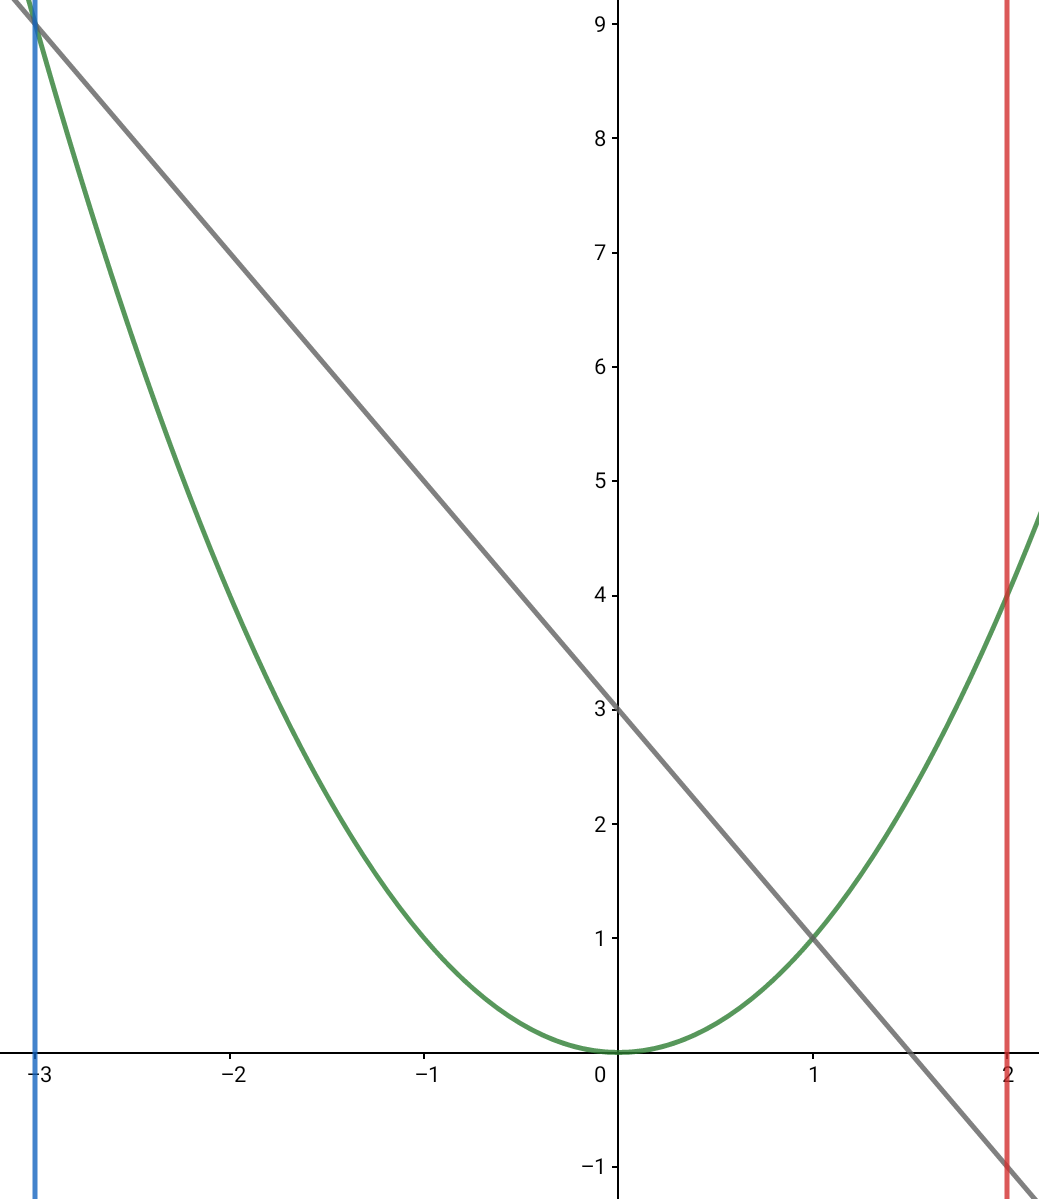
\includegraphics[width=0.5\textwidth, angle=0]{Grafico13.png}
\end{center}
\end{figure}
\par A área entre a parábola $y=x^2$ (em verde) e a reta $y=3-2x$ (em cinza) é dada por:
\begin{equation*}\displaystyle{\int_{-3}^{1} (3 - 2x - x^{2})\, dx + \int_{1}^{2} (x^{2} - 3 + 2x)\, dx = \Big( 3x - \frac{2x^2}{2} - \frac{x^3}{3}\Big)\Big|^{1}_{-3} + \Big( \frac{x^3}{3} + \frac{2x^2}{2} - 3x \Big)\Big|^{2}_{1} = 13 u.a.}\end{equation*}
\par
\vspace{0.3cm}
\begin{flushleft}
3. Calcular a área da região delimitada pelas retas $x=0$, $y=-\displaystyle{\frac{2x}{3}}$ e $y=x-5$.
\end{flushleft}
\par
\vspace{0.3cm}
\begin{flushleft}
3.1 Resolução.
\end{flushleft}
\par Calculando a interseção entre $y=-\displaystyle{\frac{2x}{3}}$ e $y=x-5$:
\begin{equation*} \displaystyle{-\frac{2x}{3} = x-5 \Leftrightarrow x=3}. \end{equation*}
\par
\vspace{1cm} Observe a figura:
\begin{figure}[htbp]
\begin{center}
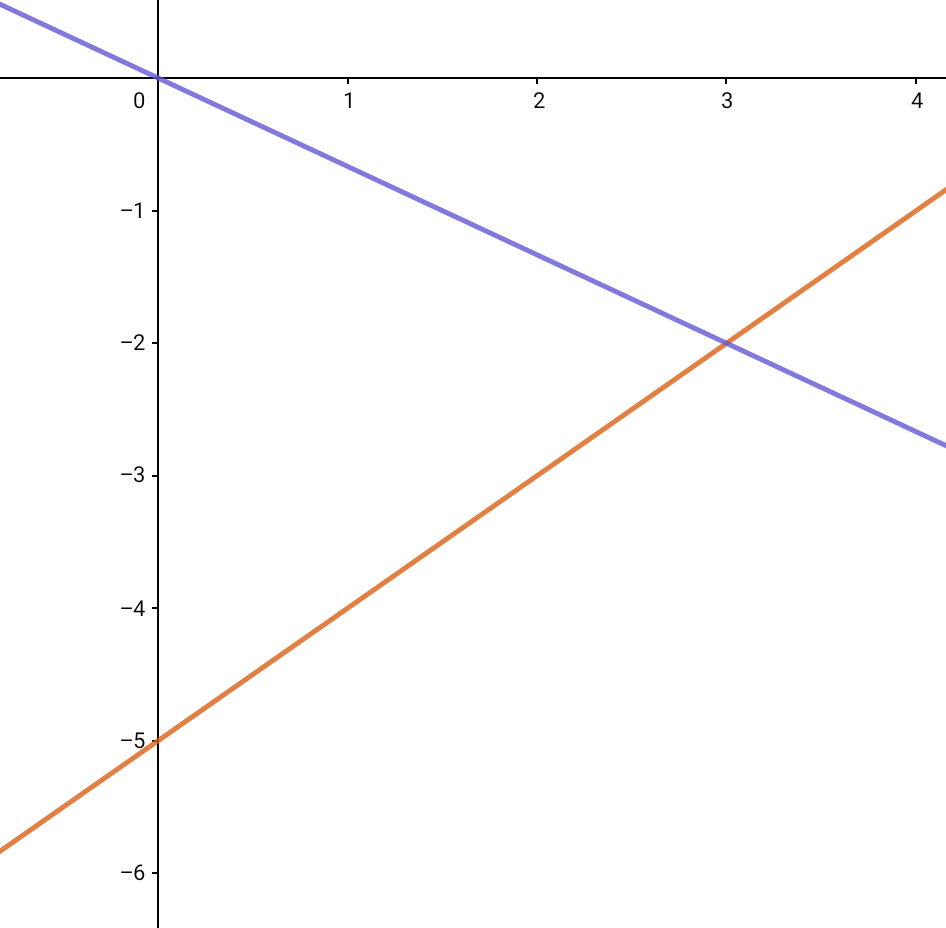
\includegraphics[width=0.5\textwidth, angle=0]{Grafico14.png}
\end{center}
\end{figure}     
\par Logo, a área desejada é dada por:
\begin{equation*} \displaystyle{-\int_{0}^{3} \Big(-\frac{2x}{3} - x + 5  \Big)\, dx = -\int_{0}^{3} \Big(-\frac{5x}{3} + 5 \Big)\, dx = -\Big(-\frac{5x^2}{6} + 5x \Big)\Big|^{3}_{0} = \frac{15}{2} u.a.}\end{equation*}
\par
\vspace{0.3cm}
\subsection{2° Teorema Fundamental do Cálculo}
\hspace{12pt} Seja $g$ uma função contínua em um intervalo $I$ e $a$ um ponto de $I$, $a$ fixo. Assim, para cada $x$ em $I$, $\displaystyle{\int_{a}^{x} g(x)\, dx}$ existe. Podemos então considerar a função que a cada $x$ em $I$ associa o número $\displaystyle{\int_{a}^{x} g(x)\, dx}$. O 2° Teorema Fundamental do Cálculo nos diz que $\displaystyle{\int_{a}^{x} g(x)\, dx}$ é uma primitiva de $g(x)$ em $I$, isto é, $\displaystyle{\frac{d}{dx}\int_{a}^{x} g(x)\, dx = g(x)}$.
\par\textbf{Demonstração}
\par Sendo $g$ contínua em $I$, é possível mostrar que existirá $G(x)$ tal que, para todo $x\in I$, $\displaystyle{\frac{d(G(x))}{dx} = G'(x) = g(x)}$. Pelo 1° Teorema Fundamental do Cálculo, $\displaystyle{\int_{a}^{x} g(x)\, dx = G(x) - G(a)}$, logo, lembrando que $G(a)$ é uma constante, temos, para todo $x$ em $I$:
\begin{equation*}\displaystyle{\frac{d}{dx}\int_{a}^{x} g(x)\, dx = \frac{d}{dx}[G(x) - G(a)] = g(x) .}\end{equation*}\begin{flushright}$\blacksquare $\end{flushright}
\par
\vspace{0.3cm}
\subsection{Propriedades da Integral}
\hspace{12pt} \textbf{Teorema}.\par Sejam $f$, $g$ integráveis em $[a;b]$ e $k$ uma constante. Então
\begin{itemize}
\item a) $f+g$ é integrável em $[a;b]$ e $\displaystyle{\int_{a}^{b}(f(x) + g(x))\, dx = \int_{a}^{b}f(x)\, dx + \int_{a}^{b}g(x)\, dx}$;
\item b) $k\cdot f$ é integrável em $[a;b]$ e $\displaystyle{\int_{a}^{b}k\cdot f(x)\, dx = k\cdot\int_{a}^{b} f(x)\, dx }$; 
\item c) Se $f(x)\geq 0$ em $[a;b]$, então $\displaystyle{\int_{a}^{b}f(x)\, dx \geq 0}$;
\item d) Se $c\in ]a;b[$ e $f$ é integrável em $[a;c]$ e em $[c;b]$, então
$\displaystyle{\int_{a}^{b} f(x)\, dx = \int_{a}^{c}f(x)\, dx + \int_{c}^{b} f(x)\, dx}$.
\end{itemize}
\par
\vspace{0.3cm}
\subsection{Técnicas de Integração}
\hspace{12pt}\textbf{I) Substituição - mudanças de variáveis}
\par A técnica, substituição, é utilizada para calcular integrais que têm a forma $\displaystyle{\int_{}^{}f(g(x))\cdot g'(x)\, dx}$
\par Sejam $y=f(x)$ e $y=g(x)$ funções tais que $f(g(x))$ existe, $f$ e $g$ contínuas, $g$ derivável e $F(x)$ uma primitiva de $f(x)$. Então, $F(g(x))$ é uma primitiva de $f(g(x))\cdot g'(x)$.
\par
\vspace{0.3cm}
\textbf{Demonstração.}
\par Note que:
\begin{equation*}\displaystyle{F'(g(x)) = F'(g(x))\cdot g'(x) = f(g(x))\cdot g'(x).}\end{equation*}
\par Assim, para calcularmos integrais que têm a forma $\displaystyle{\int_{}^{} f(g(x))\cdot g'(x)\, dx}$ fazemos $u=g(x)$ e $du=g'(x)\, dx$ para obter:
\begin{equation*} \displaystyle{\int_{}^{} f(g(x))\cdot g'(x)\, dx = \int_{}^{} f(u)\, du = F(u) + c = F(g(x)) + c, c\in\mathbb{R}}.\end{equation*}
\begin{flushright}$\blacksquare$\end{flushright}
\par
\vspace{0.3cm}
Exemplos.
\par
\begin{flushleft}
1. Calcule
\end{flushleft}
\par \begin{multicols}{4}
\hspace{-15pt}a)$\displaystyle{\int_{}^{} \frac{1}{3x-2}\, dx}$\\
b)$\displaystyle{\int_{}^{} (3x-2)^{3}}\, dx$\\
c)$\displaystyle{\int_{}^{} \frac{x}{(1 + 4x^{2})^{2}}\, dx}$\\
d)$\displaystyle{\int \frac{e^{\sqrt{x}}}{\sqrt{x}}\, dx}$\\
e)$\displaystyle{\int \frac{\sin{x}}{\cos^{2}{x}}\, dx}$\\   
f)$\displaystyle{\int x^{5}\sqrt{1 + x^{3}}\, dx}$\\
g)$\displaystyle{\int \frac{\ln^{3}{x}}{x}\, dx}$\\
h)$\displaystyle{\int \frac{\sin{\ln{x}}}{x}\, dx}$
\end{multicols}
\par
\vspace{0.3cm}
\begin{flushleft}
1.1 Resolução.
\end{flushleft}
\par a) Fazendo $3x - 2 = u$, temos:
\begin{equation*} \displaystyle{3x - 2 = u \Rightarrow 3\, dx = du \Rightarrow dx = \frac{du}{3}}. \end{equation*}
\par Substituindo na integral, vem:
\begin{equation*} \displaystyle{\int \frac{1}{3x - 2}\, dx = \int \frac{1}{u}\cdot\frac{du}{3} = \frac{1}{3}\cdot\int \frac{1}{u}\, du = \frac{1}{3}\cdot\ln{|u|} + c = \frac{1}{3}\cdot\ln{|3x-2|} + c, c\in\mathbb{R}}.\end{equation*}
\par
\vspace{0.3cm}
b) Tomando $3x - 2 = u$, segue:
\begin{equation*} 3x - 2 = u \Rightarrow 3\, dx = du \Rightarrow \displaystyle{dx = \frac{du}{3}}.\end{equation*}
$$\therefore \displaystyle{\int (3x - 2)^{3}\, dx = \int u^{3}\cdot\frac{du}{3} = \frac{1}{3}\cdot\int u^{3}\, du = \frac{1}{3}\cdot\frac{u^{4}}{4} = \frac{(3x - 2)^{4}}{12} + c, c\in\mathbb{R}}.$$
\par
\vspace{0.3cm}
c) Tome $u = 1 + 4x^2$. Logo:
\begin{equation*} u = 1 + 4x^2 \Rightarrow du = 8x\, dx \Rightarrow \displaystyle{x\, dx = \frac{du}{8}}.\end{equation*}
$$\therefore \displaystyle{\int \frac{x}{(1 + 4x^{2})^2}\, dx = \frac{1}{8}\int \frac{1}{u^2}\, du = -\frac{1}{8}\cdot\frac{1}{u} + c  = -\frac{1}{8(1 + 4x^2)} + c, c\in\mathbb{R}}.$$
\par
\vspace{0.3cm}
d) Fazendo $u = \sqrt{x}$, temos:
\begin{equation*} \displaystyle{du = \frac{1}{2\sqrt{x}} \Rightarrow \frac{dx}{\sqrt{x}} = 2\, du}.\end{equation*}
$$\therefore \displaystyle{\int \frac{e^{\sqrt{x}}}{\sqrt{x}}\, dx = 2\cdot\int e^{u}\, du = 2e^{u} + c = 2e^{\sqrt{x}} + c, c\in\mathbb{R}}.$$
\par
\vspace{0.3cm}
e) Note que $\displaystyle{\frac{\sin{x}}{\cos^{2}{x}} = \tan{x}\cdot\sec{x}}$. Tomando $\sec{x} = u$, vem:
\begin{equation*}\displaystyle{\sec{x} = u \Rightarrow \sec{x}\tan{x}\, dx = du}.\end{equation*}
$$\therefore \displaystyle{\int \sec{x}\tan{x}\, dx = \int du = u + c = \sec{x} + c, c\in\mathbb{R}}.$$
\par
\vspace{0.3cm}
f) Fazendo $u = \sqrt{1 + x^{3}}$, tem-se:
\begin{equation*} \displaystyle{du = \frac{3x^{2}}{2\sqrt{1 + x^{3}}}\, dx \Rightarrow 2u\, du = 3x^{2}\, dx \Rightarrow x^{2}\, dx = \frac{2udu}{3}}.\end{equation*}
\begin{equation*} u^{2} = 1 + x^3 \Rightarrow x^{3} = u^{2} - 1.\end{equation*}
$$ \displaystyle{\begin{split}\therefore &\int x^{5}\cdot\sqrt{1 + x^{3}}\, dx = \int (u^{2} - 1)\cdot u\cdot\frac{2u}{3}\, du = \frac{2}{3}\cdot\int u^{2}(u^2 - 1)\, du = \frac{2}{3}\Big(\frac{u^5}{5} - \frac{u^3}{3}\Big) + c = \\ = &\frac{2}{3}\Big( \frac{(1 + x^3)^{\frac{5}{2}}}{5} - \frac{(1 + x^3)^{\frac{3}{2}}}{3}\Big) + c, c\in\mathbb{R}.\end{split}}$$
\par
\vspace{0.3cm}
g) Tome $u = \ln{x}$. Daí,
\begin{equation*} \displaystyle{du = \frac{1}{x}\, dx}. \end{equation*}
$$\therefore \int \frac{\ln^{3}{x}}{x}\, dx = \int u^{3}\, du = \frac{u^{4}}{4} + c = \frac{\ln^{4}{x}}{4} + c, c\in\mathbb{R}. $$
\par
\vspace{0.3cm}
h) Fazendo $u = \ln{x}$, segue:
\begin{equation*} du = \displaystyle{\frac{1}{x}\, dx}. \end{equation*}
$$\therefore \displaystyle{\int \frac{\sin{(\ln{x})}}{x} dx = \int \sin{(u)}\, du = -\cos{u} + c = -\cos{(\ln{x})} + c, c\in\mathbb{R}}.$$
\par
\vspace{0.3cm}
\textbf{II) Integração por partes}
\par Supondo $u=u(x)$ e $v=v(x)$ definidas e deriváveis num mesmo intervalo $I$, segue da regra de derivação do produto de duas funções:
\begin{equation*}\displaystyle{\frac{d(uv)}{dx} = u\cdot\frac{dv}{dx} + v\cdot\frac{du}{dx} \Rightarrow \int \frac{d(uv)}{dx}\, dx = \int u\cdot\frac{dv}{dx}\, dx + \int v\cdot\frac{du}{dx}\, dx}.\end{equation*}
$$\therefore \displaystyle{uv = \int u\, dv + \int v\, du \Rightarrow \int u\, dv = uv - \int v\, du}.$$
\par\textbf{Observação}: quando integrando por partes, tudo se resume a qual função integrar e qual função derivar. Em alguns casos, a escolha não é tão simples e pode ser que a primeira escolha apenas complique a questão. Em outros casos, a escolha é, de certo modo, imediata.
\par
\vspace{0.3cm}
Exemplos.
\par
\begin{flushleft}
1. Calcule
\end{flushleft}  
\par
\begin{multicols}{3}
\hspace{-15pt}a)$\displaystyle{\int \ln{x}\, dx}$\\
b)$\displaystyle{\int \arctan{x}\, dx}$\\
c)$\displaystyle{\int xe^{x}\, dx}$
\end{multicols}
\par
\vspace{0.3cm}
\begin{flushleft}
1.1 Resolução.
\end{flushleft}
\par
a) Tomando $u=\ln{x}$ e $dx=dv$, temos:
\begin{equation*}\displaystyle{du = \frac{1}{x}\, dx, v = x}.\end{equation*}
$$\therefore \displaystyle{\int \ln{x}\, dx = x\ln{x} - \int x\cdot\frac{1}{x} dx = x\ln{x} - x + c, c\in\mathbb{R}}.$$
\par
\vspace{0.3cm}
b) Fazendo $\arctan{x} = u$ e $dx = dv$, segue:
\begin{equation*} \displaystyle{du = \frac{1}{1+x^2}\, dx, v = x}.\end{equation*}
\begin{equation*}\therefore \displaystyle{\int \arctan{x}\, dx = x\arctan{x} - \int \frac{x}{1+x^2}\, dx }.\end{equation*}
\par Calculando $\displaystyle{\int \frac{x}{1+x^2}\, dx}$ por substituição, obtemos $\displaystyle{\frac{1}{2}\cdot\ln{(1 + x^2)} + c, c\in\mathbb{R}}$.
$$\therefore \displaystyle{\int \arctan{x}\, dx = x\arctan{x} - \frac{1}{2}\ln{(1 + x^{2})} + c,c\in\mathbb{R}}.$$
\par
\vspace{0.3cm}
c) Tome $x=u$ e $dv = e^{x}\, dx$. Daí:
\begin{equation*} \displaystyle{dx = du, v = e^{x} }.\end{equation*}
$$\therefore \displaystyle{\int xe^{x}\, dx = xe^{x} - \int e^{x}\, dx = xe^{x} - e^{x} = e^{x}(x-1) + c, c\in\mathbb{R}}.$$
\par
\vspace{0.3cm}
\begin{flushleft}
2. a) Verifique que $\displaystyle{\int \sin^{n}{x}\, dx = -\frac{1}{n}\cdot\sin^{n-1}{x}\cdot\cos{x} + \frac{n-1}{n}\cdot\int \sin^{n-2}{x}\, dx, \forall n\in\mathbb{N}, n\geq 2}.$
\par\hspace{12pt}b) Calcule $\displaystyle{\int \sin^{6}{x}\, dx}$.
\end{flushleft}
\par
\vspace{0.3cm}
\begin{flushleft}
2.1 Resolução.
\end{flushleft}
\par a) Note que $\displaystyle{\int \sin^{n}{x}\, dx = \int \sin^{n-1}{x}\cdot\sin{x}\, dx}$. Tomando $u=\sin^{n-1}{x}$ e $dv = \sin{x}\, dx$, segue:
\begin{equation*}\displaystyle{du = (n-1)\sin^{n-2}{x}\cdot\cos{x}\, dx , v = -\cos{x}}. \end{equation*}
$$\displaystyle{\begin{split}\therefore \int \sin^{n}{x}\, dx &= -\sin^{n-1}{x}\cdot\cos{x} + \int (n-1)\cdot\cos{x}\cdot\sin^{n-2}{x}\cdot\cos{x}\, dx               
= \\ =& -\sin^{n-1}{x}\cdot\cos{x} + (n-1)\int (1 - \sin^{2}{x})\sin^{n-2}{x}\, dx = \\ = &-\sin^{n-1}{x}\cdot\cos{x} + (n-1)\int \sin^{n-2}{x}\, dx - (n-1)\int \sin^{n}{x}\, dx.\end{split}}$$
\par Daí, tiramos:
$$\displaystyle{\begin{split}\therefore &\, n\cdot\int \sin^{n}{x}\, dx = -\sin^{n-1}{x}\cdot\cos{x} + (n-1)\int \sin^{n-2}{x}\, dx \\ \Rightarrow &\int \sin^{n}{x}\, dx = -\frac{1}{n}\cdot\sin^{n-1}{x}\cdot\cos{x} + \frac{n-1}{n}\cdot\int \sin^{n-2}{x}\, dx.\end{split}}$$\begin{flushright}$\blacksquare$\end{flushright}
\par
\vspace{0.3cm}
b) Aplicando a fórmula que acabamos de deduzir, vem:
\begin{equation*} \displaystyle{\begin{split} &\int\sin^{6}{x}\, dx = -\frac{1}{6}\cdot\sin^{5}{x}\cos{x} + \frac{5}{6}\cdot\int\sin^{4}{x}\, dx = \\ = &-\frac{1}{6}\cdot\sin^{5}{x}\cos{x} + \frac{5}{6}\Big(-\frac{1}{4}\cdot\sin^{3}{x}\cos{x} + \frac{3}{4}\cdot\int\sin^{2}{x}\, dx\Big) = \\ = &-\frac{1}{6}\cdot\sin^{5}{x}\cos{x} - \frac{5}{24}\sin^{3}{x}\cos{x}+\frac{5}{8}\cdot\Big(-\frac{1}{2}\sin{x}\cos{x} + \frac{1}{2}\int dx\Big) = \\ = &-\frac{1}{6}\cdot\sin^{5}{x}\cos{x} - \frac{5}{24}\sin^{3}{x}\cos{x} - \frac{5}{16}\sin{x}\cos{x} + \frac{5x}{16} + c, c\in\mathbb{R}
.\end{split}}\end{equation*}
\par
\vspace{0.3cm}
\begin{flushleft}
3. Calcule
\end{flushleft}
\par
\begin{multicols}{3}
\hspace{-15pt}a)$\displaystyle{\int x^{2}\ln{x}\, dx}$\\
b)$\displaystyle{\int xe^{2x}\, dx}$\\
c)$\displaystyle{\int e^{x}\cos{x}\, dx}$
\end{multicols}
\par
\vspace{0.3cm}
\begin{flushleft}
3.1 Resolução.
\end{flushleft}
\par a) Fazendo $u = \ln{x}$ e $dv = x^{2}\, dx$, temos:
\begin{equation*} \displaystyle{du = \frac{1}{x}\, dx, v = \frac{x^3}{3}}.\end{equation*}
$$\displaystyle{\therefore \int x^{2}\ln{x}\, dx = \frac{x^3}{3}\cdot\ln{x} - \frac{1}{3}\cdot\int x^{3}\cdot\frac{1}{x}\, dx = \frac{x^3}{3}\cdot \Big(\ln{x} - \frac{1}{3}\Big) + c, c\in\mathbb{R}.}$$
\par
\vspace{0.3cm}
b) Tomando $u = x$ e $dv = e^{2x}\, dx$, segue:
\begin{equation*} du = dx, v = \displaystyle{\frac{e^{2x}}{2}}.\end{equation*}
$$\displaystyle{\therefore \int xe^{2x}\, dx = x\cdot\frac{e^{2x}}{2} - \frac{1}{2}\cdot\int e^{2x}\, dx = \frac{e^{2x}}{2}\cdot\Big( x - \frac{1}{2}\Big) + c, c\in\mathbb{R}.}$$
\par
\vspace{0.3cm}
c) Tome $u = e^{x}$ e $dv = \cos{x}\, dx$. Daí:
\begin{equation*}\displaystyle{du = e^{x}dx , v = \sin{x}.}\end{equation*}
\par
\begin{equation*} \displaystyle{\therefore \int e^{x}\cos{x}\, dx = e^{x}\sin{x} - \int e^{x}\sin{x}\, dx}.\end{equation*}
\par Agora, vamos integrar $e^{x}\sin{x}$ por partes. Tomando $u = e^{x}$ e $d\sigma = \sin{x}\, dx$, vem:
\begin{equation*} du = e^{x}\, dx , \sigma = -\cos{x} . \end{equation*}
\par Logo:
\begin{equation*}\displaystyle{\int e^{x}\sin{x}\, dx = -e^{x}\cos{x} + \int e^{x}\cos{x}\, dx}.\end{equation*}
$$\displaystyle{\therefore \int e^{x}\cos{x}\, dx = e^{x}\sin{x} + e^{x}\cos{x} - \int e^{x}\cos{x}\, dx \Rightarrow \int e^{x}\cos{x}\, dx = \frac{e^{x}}{2}\cdot (\sin{x} + \cos{x}) + c, c\in\mathbb{R}.}$$
\par
\vspace{0.3cm}
\begin{flushleft}
4. Verifique que $\forall n\in\mathbb{N}, n\geq 1$ e $\forall s\in\mathbb{R^{*}_{+}}$, vale:
\begin{equation*} \displaystyle{\int t^{n}\cdot e^{-st}\, dt = -\frac{1}{s}\cdot t^{n}\cdot e^{-st} + \frac{n}{s}\cdot\int t^{n-1}\cdot e^{-st}\, dt.}\end{equation*}
\end{flushleft}              
\par
\vspace{0.3cm}
\begin{flushleft}
4.1 Resolução.
\end{flushleft}
\par Tomando $u = t^{n}$ e $dv = e^{-st}\, dt$, segue:
\begin{equation*}\displaystyle{du = nt^{n-1} , v = -\frac{e^{-st}}{s}.}\end{equation*}
$$\displaystyle{\therefore \int t^{n}\cdot e^{-st}\, dt =  -\frac{1}{s}\cdot t^{n}\cdot e^{-st} + \frac{n}{s}\cdot\int t^{n-1}\cdot e^{-st}\, dt.}$$
\par
\vspace{0.3cm}
\textbf{III) Frações Parciais}   
\par \textbf{Teorema}.\par
Sejam $m$, $n$, $\alpha $ e $\beta $, com $\alpha\neq\beta $, números reais dados. Então, existem números reais $A$ e $B$ tais que:
\begin{itemize}
\item $\displaystyle{\frac{mx + n}{(x-\alpha )(x-\beta )} = \frac{A}{x-\alpha } + \frac{B}{x-\beta }}$;
\item $\displaystyle{\frac{mx+n}{(x-\alpha )^2} = \frac{A}{x-\alpha } + \frac{B}{(x-\alpha )^2}}$.
\end{itemize}
\par\textbf{Observações}: para utilizar esta técnica, o grau do polinômio no numerador deve ser estritamente menor que o grau do polinômio no denominador. Caso o grau do polinômio no numerador seja maior ou igual ao grau do denominador, é necessário dividir o numerador pelo denominador e "extrair os inteiros''. Além disso, esta técnica é aplicável para polinômios de qualquer grau, basta continuar escrevendo os fatores cujos denominadores são os monômios formadores do denominador. Caso o denominador seja do tipo $(x-\alpha )(x-\beta )^{2}$, por exemplo, serão necessários 3 frações: uma com denominador $(x-\alpha )$, outra com denominador $(x-\beta )$ e a última com denominador $(x-\beta )^2$. Nesse caso, é necessário ''construir'' as potências (o raciocínio se mantém para raízes de multiplicidade maior que 2). Por fim, caso o denominador seja um polinômio que apresente fatores irredutíveis (por exemplo, um polinômio do 2° grau com $\Delta < 0$), trate o fator irredutível como se fosse um dos monômios apresentados acima, isto é, para $m$, $n$, $p$, $a$, $b$, $c$ e $\alpha $ números reais dados e $\Delta = b^{2} - 4ac < 0$, Existem constantes $A$, $B$ e $D$ tais que $\displaystyle{\frac{mx^{2} + nx + p}{(x-\alpha )(ax^{2} + bx + c)} = \frac{A}{x-\alpha } + \frac{Bx + D}{ax^{2} + bx + c}}$.
\par
\vspace{0.3cm}
Exemplos.
\par
\begin{flushleft}
1. Calcule:
\end{flushleft}
\par
\begin{multicols}{3}
a)$\displaystyle{\int \frac{dx}{x^2 - 4}}$\\
b)$\displaystyle{\int \frac{x^2 + x + 1}{x^2 - 5x + 6}\, dx}$\\
c)$\displaystyle{\int \sec{x}\, dx}$
\end{multicols}
\par
\vspace{0.3cm}
\begin{flushleft}
1.1 Resolução.
\end{flushleft}
\par a) Sendo $x^2 - 4 = (x-2)(x+2)$, temos, para $A$ e $B$ constantes reais:
\begin{equation*}\displaystyle{\begin{split}
\frac{1}{x^2 - 4} &= \frac{1}{(x-2)(x+2)}=\frac{A}{x-2} + \frac{B}{x+2} \\
\Leftrightarrow \frac{1}{x^2 - 4} &= \frac{A(x+2) + B(x-2)}{(x-2)(x+2)} \\ \Leftrightarrow 1&\equiv A(x+2) + B(x-2) \\
\Leftrightarrow A&=\frac{1}{4}, B=-\frac{1}{4}.
\end{split}}\end{equation*}
$$\displaystyle{\begin{split}
\therefore \int \frac{1}{x^2 - 4}\, dx &= \int\Big( \frac{\frac{1}{4}}{x-2} + \frac{-\frac{1}{4}}{x+2}  \Big)\, dx = \\
&=\frac{1}{4}\cdot\int \frac{1}{x-2}\, dx-\frac{1}{4}\cdot\int \frac{1}{x+2}\, dx = \\
&=\frac{1}{4}\cdot\ln{|x-2|}-\frac{1}{4}\cdot\ln{|x+2|}= \\
&=\frac{1}{4}\cdot\ln{\Big|\frac{x-2}{x+2}\Big|}+ c, c\in\mathbb{R}.      \end{split}}$$ 
\par
\vspace{0.3cm}
b) $\displaystyle{\int \frac{x^2 + x + 1}{x^2 - 5x + 6}\, dx = \int \frac{(x^2 - 5x + 6) + 6x - 5}{x^2 - 5x + 6}\, dx = \int dx + \int \frac{6x - 5}{(x-2)(x-3)}\, dx = x + \int \frac{6x-5}{(x-2)(x-3)}\, dx}.$
\par\vspace{0.2cm}
Reescrevendo $\displaystyle{\frac{6x-5}{(x-2)(x-3)}}$ utilizando frações parciais, segue:
\begin{equation*}\displaystyle{\begin{split} &\frac{6x-5}{(x-2)(x-3)} = \frac{A}{x-2} + \frac{B}{x-3} = \frac{A(x-3) + B(x-2)}{(x-2)(x-3)}  \\ &\Leftrightarrow 6x-5\equiv A(x-3) + B(x-2) \\ &\Leftrightarrow A=-7, B=13.
\end{split}}\end{equation*}
$$\displaystyle{\therefore x + \int \frac{6x-5}{(x-2)(x-3)}\, dx = x - 7\cdot\int \frac{1}{x-2}\, dx + 13\cdot\int \frac{1}{x-3}\, dx = x - 7\cdot\ln{|x-2|} + 13\cdot\ln{|x-3|} + c, c\in\mathbb{R}.}$$
\par
\vspace{0.3cm}
c) $\displaystyle{\int \sec{x}\, dx = \int \frac{1}{\cos{x}}\, dx = \int \frac{\cos{x}}{\cos^{2}{x}}\, dx = \int \frac{\cos{x}}{1 - \sin^{2}{x}}\, dx}$
\par\vspace{0.2cm}
Tomando $u=\sin{x}$, segue que $du = \cos{x}\, dx$. Daí:
\begin{equation*}\displaystyle{\int \sec{x}\, dx = \int \frac{\cos{x}}{1 - \sin^{2}{x}}\, dx = \int \frac{1}{1-u^2}\, du}.\end{equation*}
\par Reescrevendo $\displaystyle{\frac{1}{1-u^2}}$, vem:
\begin{equation*}\displaystyle{\frac{1}{1-u^2} = \frac{A}{1-u} + \frac{B}{1+u} \Leftrightarrow 1\equiv A(1+u) + B(1-u) \Leftrightarrow A=B=\frac{1}{2}.}\end{equation*}
$$\displaystyle{\begin{split}\therefore \int\sec{x}\, dx &= \frac{1}{2}\cdot\int \frac{1}{1+u}\, du-\frac{1}{2}\cdot\int-\frac{1}{1-u}\, du = \\ 
&=\frac{1}{2}\cdot\ln{|1+u|} - \frac{1}{2}\cdot\ln{|1-u|} = \\ &= \frac{1}{2}\cdot\ln{\Big|\frac{1+\sin{x}}{1-\sin{x}}\Big|} = \\ &= \frac{1}{2}\cdot\ln{\Big| \frac{1 + 2\sin{x} + \sin^{2}{x}}{1 - \sin^{2}{x}}\Big|} = \\ &=\frac{1}{2}\cdot\ln{|\sec^{2}{x} + 2\sec{x}\tan{x} + \tan^{2}{x}|} = \\ &=\ln{|\sec{x} + \tan{x}|+c,c\in\mathbb{R}.}\end{split}}$$
\par
\vspace{0.3cm}
\subsection{Volume de sólido obtido pela rotação de um conjunto $A$ em torno do eixo $x$}
\hspace{12pt} Seja $f$ contínua em $[a;b]$, $f(x)\geq 0$ em $[a;b]$. Seja $B$ o sólido obtido pela rotação, em torno do eixo $x$, do conjunto $A$ do plano limitado pelas retas $x=a$ e $x=b$. Queremos definir o volume $V$ de $B$.
\par Observe as figuras 12 e 13.
\begin{figure}[htbp]
\begin{center}
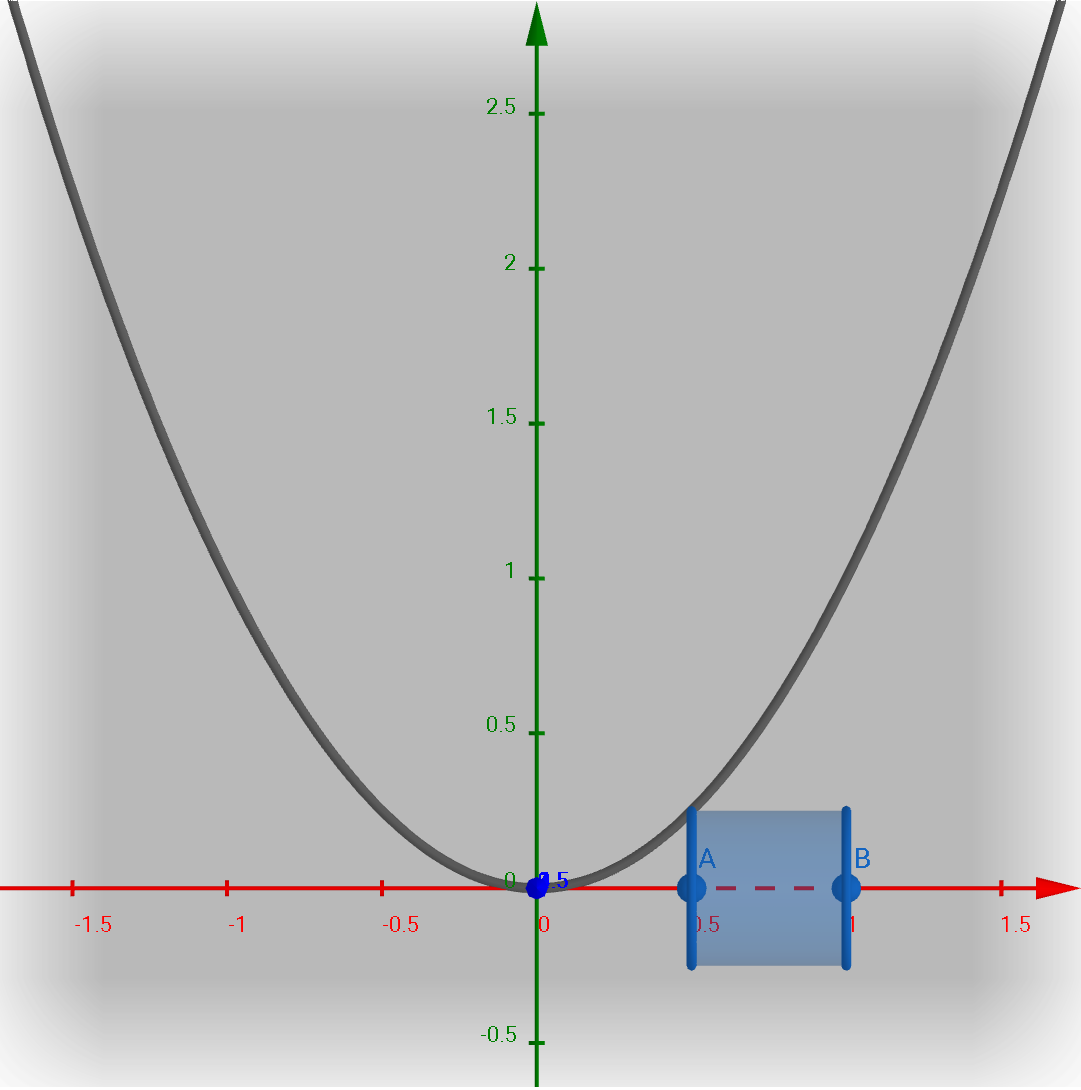
\includegraphics[width=0.4\textwidth, angle=0]{Grafico15.png}
\end{center}
\caption{}
\end{figure}

\begin{figure}[htbp]
\begin{center}
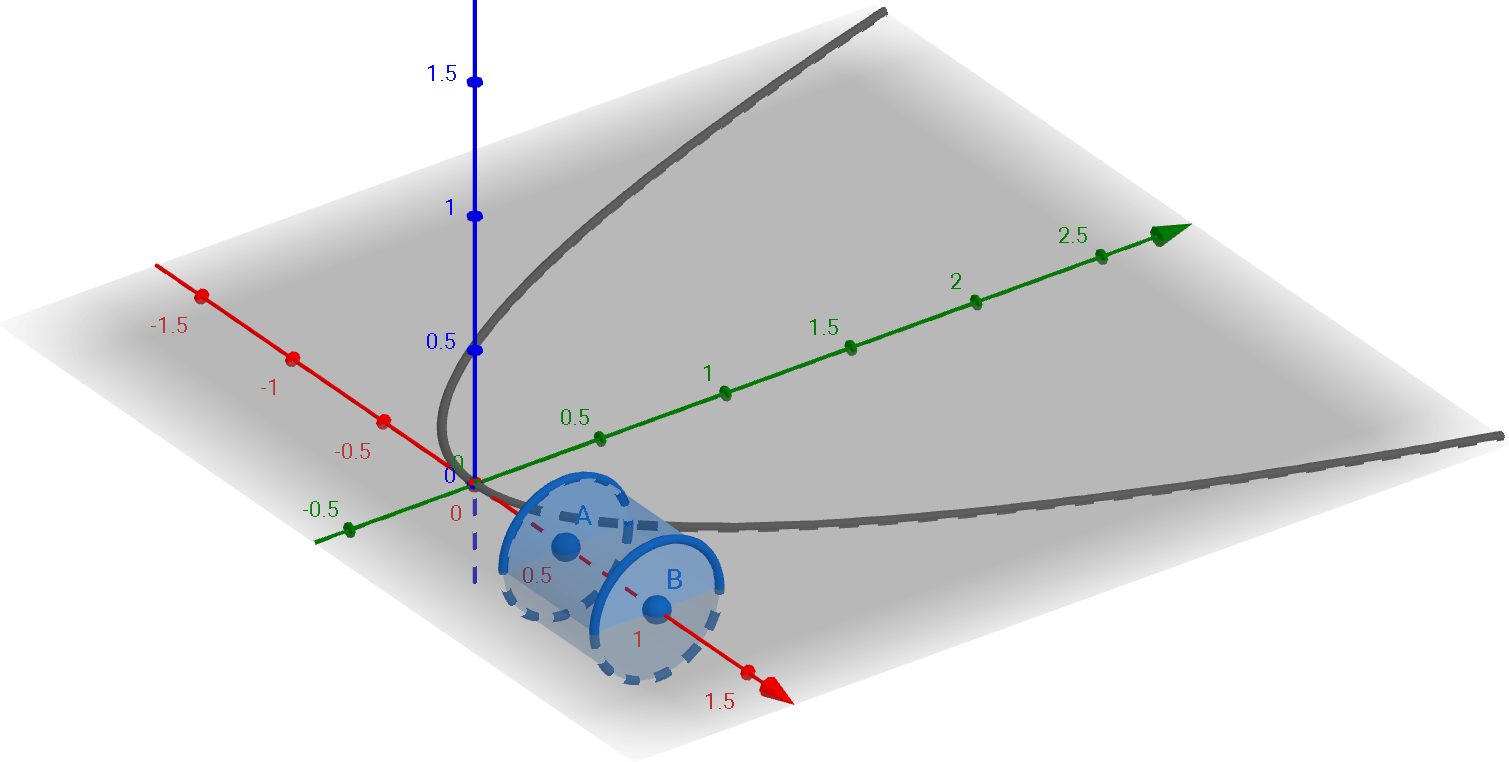
\includegraphics[width=0.6\textwidth, angle=0]{Grafico16.png}
\end{center}
\caption{}
\end{figure}

\par Note que o cilindro azul se aproxima do volume do sólido obtido pela rotação, em torno do eixo $x$, da parábola $y=x^2$. Agora, imagine que temos $n$ cilindros (também obtidos através de rotação) num intervalo $[a;b]$ de uma função $f$ contínua em $[a;b]$. O volume de $B$ será aproximadamente igual a soma dos volumes dos cilindros, isto é, $V\approx \displaystyle{\sum_{i=1}^{n}C_i}$, em que $C_i$ é o volume de cada cilindro. Suponha, sem perda de generalidade, que os cilindros tenham todos a mesma altura, isto é, a nossa partição $P:a= x_0 < x_1 < x_2 < \cdots < x_{i-1} < x_i < \cdots x_n =b$ de $[a;b]$ possui subintervalos de mesmo comprimento. Chamando de $\Delta x$ o comprimento de cada subintervalo, note que o volume de $B$ será dado por $\displaystyle{V = \lim_{n\to \infty }\sum_{i=1}^{n} \pi\cdot f^{2}(x_{i})\cdot\Delta x}$  que, pela definição de integral definida, se torna $$V=\pi\cdot\int_{a}^{b} f^{2}(x)\, dx.$$
\par
\vspace{0.3cm}
\textbf{Teorema de Papus}.\par
É possível mostrar que o volume do sólido obtido pela rotação, em torno de um eixo, de uma figura plana que não intercepta tal eixo é igual ao produto da área da figura pelo comprimento da circunferência formada, na rotação, pelo centro de massa (ou baricentro) da figura. Esse teorema será utilizado na próxima seção para demonstrar o volume do sólido obtido a partir da rotação, em torno do eixo $y$, de um conjunto $A$ do plano.
\par
\vspace{0.3cm}
Exemplos.
\par
\begin{flushleft}
1. Calcule o volume do sólido obtido pela rotação, em torno do eixo $x$, do conjunto de todos os pares $(x,y)$ tais que   
\end{flushleft}
\par
\begin{multicols}{3}
\hspace{-15pt}a) $\displaystyle{1\leq x\leq 3}$ e $\displaystyle{0\leq y\leq x}$\\
b) $\displaystyle{\frac{1}{2}\leq x\leq 2}$ e $\displaystyle{0\leq y\leq\frac{1}{x^2}}$\\
c) $\displaystyle{2x^{2} + y^{2}\leq 1}$ e $\displaystyle{y\geq 0}$
\end{multicols}
\par
\vspace{0.3cm}
\begin{flushleft}
1.1 Resolução.
\end{flushleft}
\par a) Os pares $(x,y)$ tais que $\displaystyle{1\leq x\leq 3}$ e $\displaystyle{0\leq y\leq x}$ definem a região delimitada pelas retas $y=x$, $x=1$ e $x=3$ e pelo eixo $x$. Observe a figura para melhor visualização.
\begin{figure}[htbp]
\begin{center}
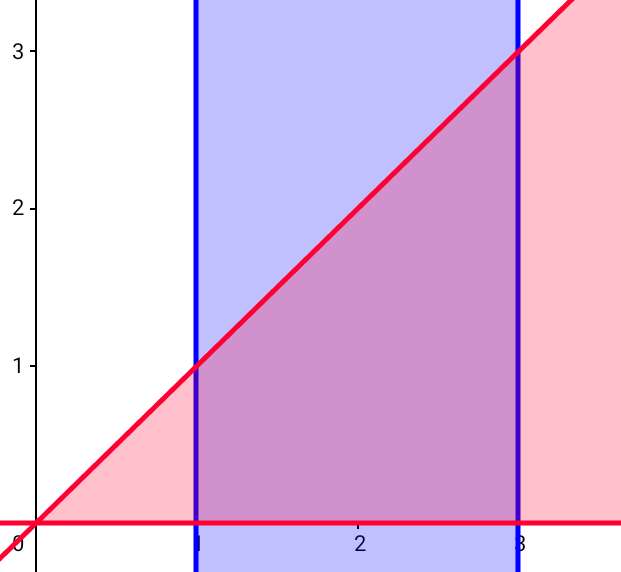
\includegraphics[width=0.5\textwidth, angle=0]{Grafico17.png}
\end{center}
\end{figure}
\par Daí, segue que o volume desejado será dado por:
\begin{equation*}\displaystyle{V = \pi\cdot\int_{1}^{3} x^{2}\, dx = \pi\cdot \Big(\frac{x^{3}}{3}\Big)\Big|^{3}_{1} = \frac{26\pi }{3}.}\end{equation*}
\par
\vspace{0.3cm}
b) Os pares $(x,y)$ tais que $\displaystyle{\frac{1}{2}\leq x\leq 2}$ e $\displaystyle{0\leq y\leq \frac{1}{x^2}}$ definem a região delimitada pelas retas $x=1$ e $x=4$, pelo gráfico de $y=\displaystyle{\frac{1}{x^2}}$ e pelo eixo $x$. Observe a figura 14 para melhor visualização.
\begin{figure}[htbp]
\begin{center}
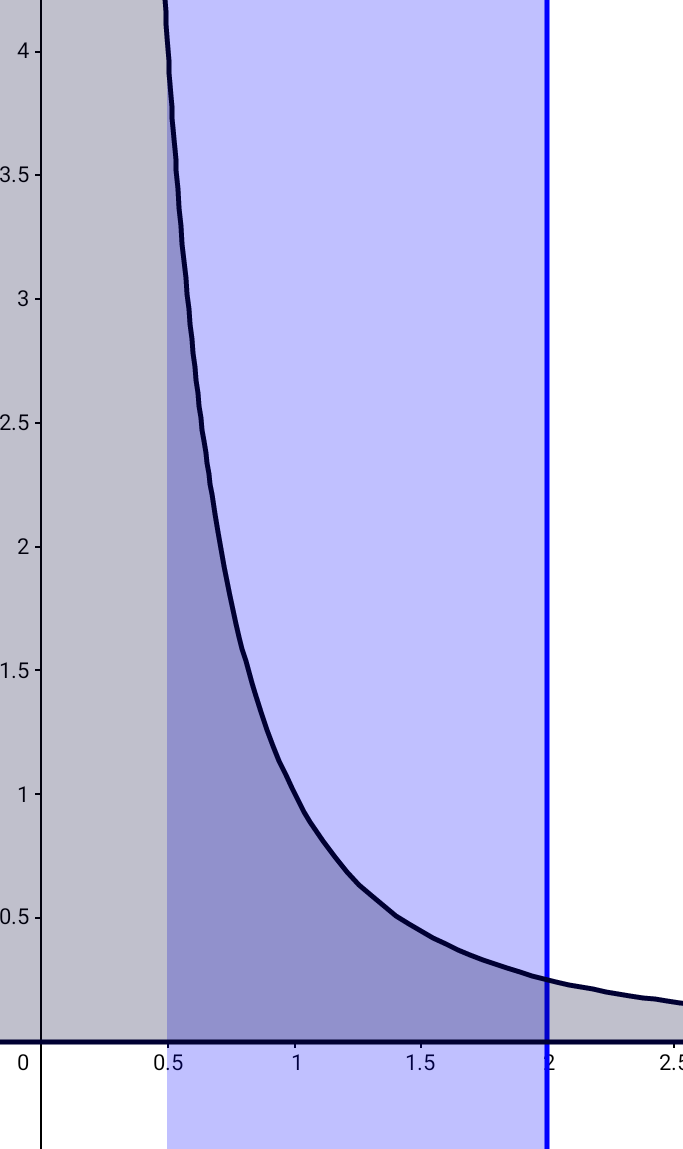
\includegraphics[width=0.4\textwidth, angle=0]{Grafico18.png}
\end{center}
\caption{}
\end{figure}
\par Logo, o volume desejado será:
\begin{equation*}\displaystyle{V = \pi\cdot\int_{\frac{1}{2}}^{2} \Big(\frac{1}{x^{2}}\Big)^{2}\, dx = \pi\cdot\int_{\frac{1}{2}}^{2} \frac{1}{x^{4}}\, dx = \pi\cdot \Big(-\frac{1}{3x^{3}}\Big)\Big|^{2}_{\frac{1}{2}} = \frac{21\pi }{8}.}\end{equation*}
\par
\vspace{0.3cm}
c) Note que se $\displaystyle{2x^2 + y^2 \leq 1}$ e $\displaystyle{y\geq 0}$, podemos escrever: $\displaystyle{y=\sqrt{1 - 2x^{2}}, -\frac{1}{\sqrt{2}}\leq x\leq \frac{1}{\sqrt{2}}}$. Observe a figura 15 para melhor visualização.
\begin{figure}[htbp]
\begin{center}
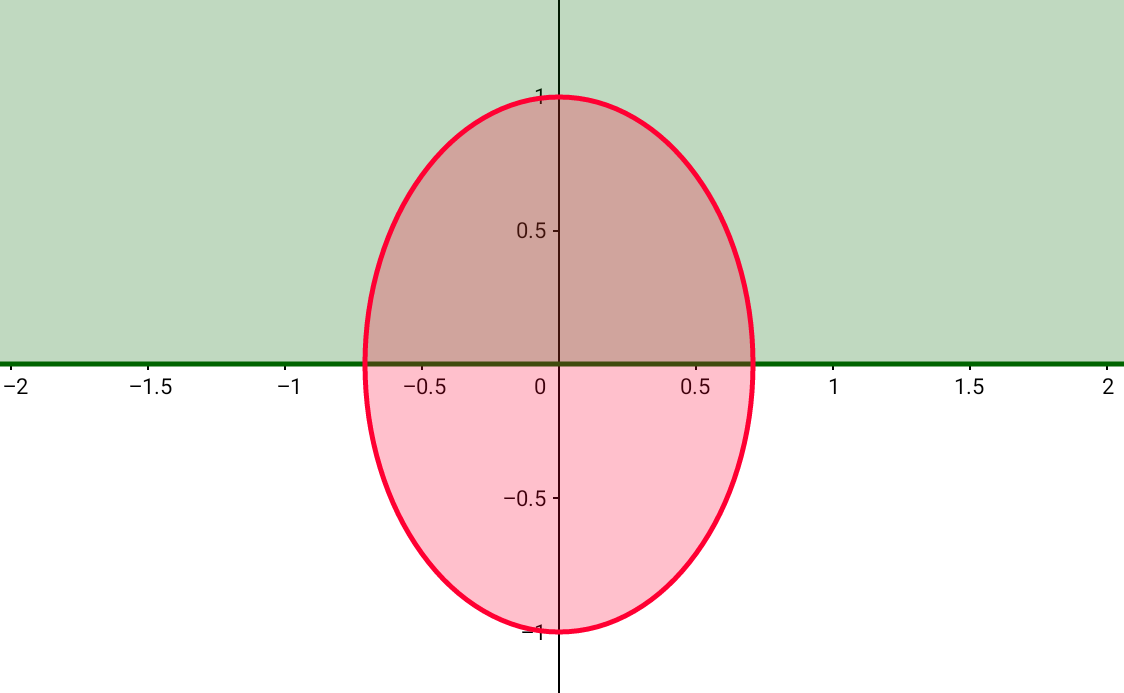
\includegraphics[width=0.5\textwidth, angle=0]{Grafico19.png}
\end{center}
\caption{}
\end{figure}
\par Por isso, temos que o volume pedido é:
\begin{equation*}\displaystyle{V = \pi\cdot\int_{-\frac{1}{\sqrt{2}}}^{\frac{1}{\sqrt{2}}} (1 - 2x^{2})\, dx = \pi\cdot\Big( x - \frac{2x^{3}}{3}\Big)\Big|^{\frac{1}{\sqrt{2}}}_{-\frac{1}{\sqrt{2}}} = \frac{2\sqrt{2}\pi}{3}.}\end{equation*}
\par
\vspace{0.3cm}
\subsection{Volume de sólido obtido pela rotação de um conjunto $A$ em torno do eixo $y$}
\hspace{12pt} Seja $f(x)\geq 0$ e contínua em $[a;b]$, com $a>0$. Seja $A$ o conjunto do plano de todos os pares $(x,y)$ tais que $\displaystyle{a\leq x\leq b}$ e $\displaystyle{0\leq y\leq f(x)}$. Seja $B$ o conjunto obtido pela rotação, em torno do eixo $y$, do conjunto $A$. Vamos mostrar que o volume $V$ de $B$ é igual a
$$\displaystyle{2\pi\cdot\int_{a}^{b}xf(x)\, dx.}$$
\par Observe a imagem.
\begin{figure}[htbp]
\begin{center}
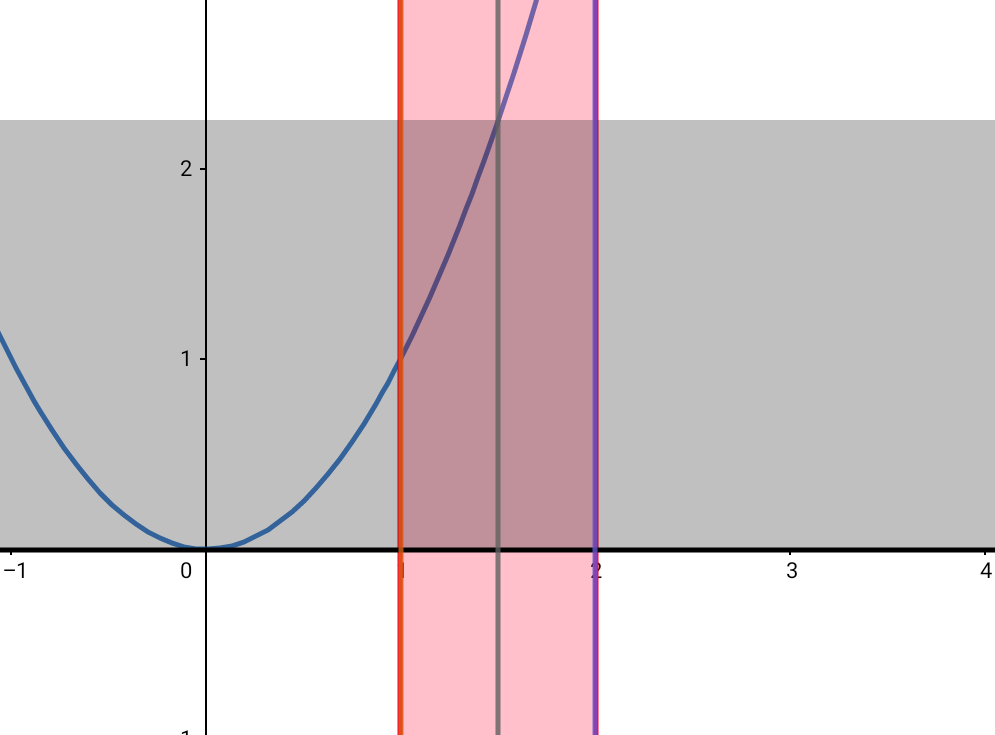
\includegraphics[width=0.5\textwidth, angle=0]{Grafico20.png}
\end{center}
\caption{note o retângulo formado pela intersecção entre $\displaystyle{0\leq y\leq 1,5^{2}}$ e $\displaystyle{1\leq x\leq 2}$.}
\end{figure}
\par
\textbf{Demonstração.}
\par
Seja $\displaystyle{P:a = x_0 < x_1 < x_2 < \cdots < x_{i-1} < x_i < \cdots < x_n = b}$ uma partição de $[a;b]$ e seja $c_i$ o ponto médio de $[x_{i-1};x_i]$. Suponha também que cada subintervalo de $[a;b]$ tem o mesmo comprimento, $\displaystyle{\Delta x = x_i - x_{i-1}}$. Seja $R_i$ o retângulo $\displaystyle{x_{i-1}\leq x\leq x_i}$ e $\displaystyle{0\leq y\leq f(c_i)}$. Pelo teorema de Papus, o volume do sólido gerado pela rotação, em torno do eixo $y$, de $R_i$ é
$$\displaystyle{2\pi c_{i}f(c_i)\Delta x}.$$
\par Assim, estamos interessados na soma dos volumes dos sólidos gerados a partir de cada retângulo formado na partição, isto é, queremos
$$\displaystyle{\sum_{i=1}^{n} 2\pi c_{i}f(c_i)\Delta x}.$$    
\par Contudo, esse somatório nos dá apenas um valor aproximado, e não exato, do volume. Aplicando o limite para $n\rightarrow \infty $, teremos o valor exato de $V$, que será:
$$\displaystyle{\lim_{n\to\infty } \sum_{i=1}^{n} 2\pi c_{i}f(c_i)\Delta x =  2\pi\cdot\int_{a}^{b}xf(x)\, dx.}$$\begin{flushright} $_{\blacksquare }$ \end{flushright}
\vspace{0.3cm}
\par\textbf{Observação 1:} é possível deduzir essa fórmula utilizando o volume de cascas/invólucros cilíndricas(os). O volume de cada invólucro será $\displaystyle{\pi\cdot f(x_i)(x_i - x_{i-1})(x_i + x_{i-1})}$. Note que somando os volumes e aplicando o limite para $n\rightarrow \infty $, $x_i + x_{i-1}$ tende a $2x$ e, portanto, teremos:
$$\displaystyle{\lim_{n\to\infty } 2\pi\sum_{i=1}^{n}xf(x_i)\Delta x       = 2\pi\cdot\int_{a}^{b}}xf(x)\, dx.$$
\par\textbf{Observação 2:} em situações que solicitem o volume obtido a partir da rotação, em torno do eixo $y$, de uma região $C$ do plano delimitada por $\displaystyle{c\leq y\leq d}$, $\displaystyle{0\leq x\leq b}$ e $\displaystyle{y\geq f(x)}$, com $f(a) = c$ e $f(b)=d$, basta fazer:
$$\displaystyle{\pi b^{2}(d-c) - 2\pi\cdot\int_{a}^{b}xf(x)\, dx + \pi\cdot c(b^{2}-a^{2})}.$$ \begin{center} Dica: esboçe o gráfico e pense no volume desejado em termos de uma diferença de volumes. \end{center}  

\par
\vspace{0.3cm}
Exemplos.
\par
\begin{flushleft}
1. Calcule o volume do sólido obtido pela rotação, em torno do eixo $y$, do conjunto de todos os $(x,y)$ tais que
\end{flushleft}
\par a) $\displaystyle{1\leq x\leq e}$ e $\displaystyle{0\leq y\leq\ln{x}}$
\hspace{0.3cm}
b) $\displaystyle{0\leq x\leq\pi}$ e $\displaystyle{0\leq y\leq\sin{x}}$
\hspace{0.3cm}
c) $\displaystyle{0\leq x\leq 1}$ e $\displaystyle{x\leq y\leq x^{2} + 1}$
\par
\vspace{0.3cm}
\begin{flushleft}
1.1 Resolução.
\end{flushleft}
\par a) O volume desejado será:
\begin{equation*}\displaystyle{2\pi\cdot\int_{1}^{e} x\ln{x}\, dx}.\end{equation*}
\par Integrando por partes, obtemos:
\begin{equation*}\displaystyle{2\pi\cdot\Big( \frac{1}{2}\cdot x^{2}\ln{}x - \frac{1}{4}\cdot x^{2}\Big)\Big|^{e}_{1} = \pi\cdot\Big(\frac{e^{2}+1}{2}\Big)} .\end{equation*}
\par Observe o gráfico para melhor visualização.
\begin{figure}[htbp]
\begin{center}
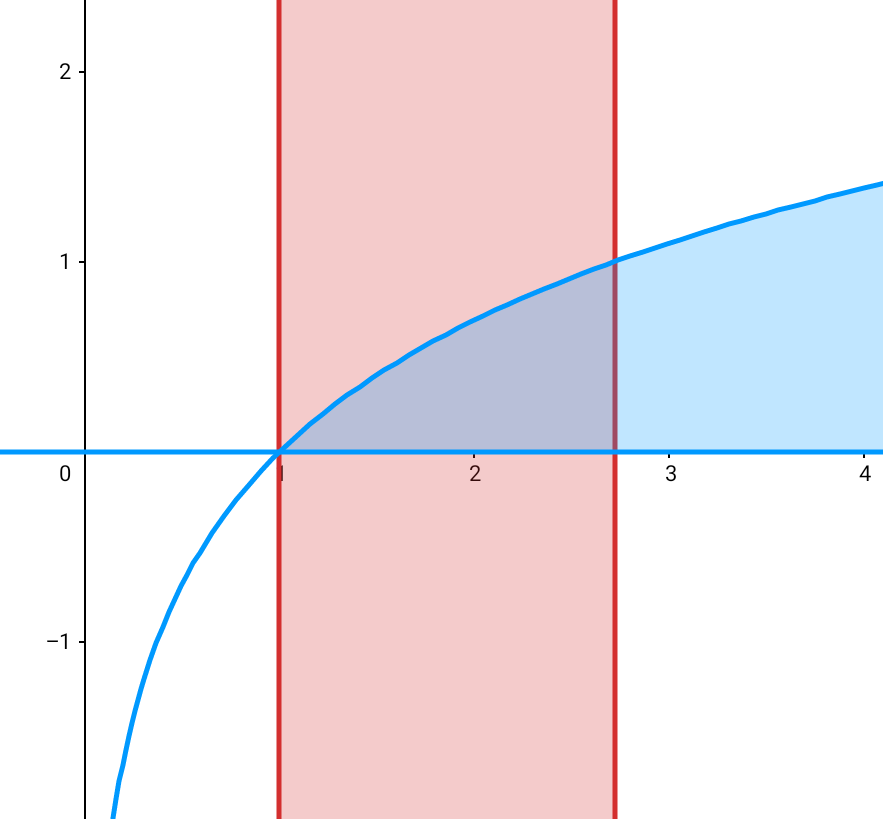
\includegraphics[width=0.5\textwidth, angle=0]{Grafico21.png}
\end{center}  
\end{figure}
\par
\vspace{0.3cm}
b) Note que o volume pedido é igual a:
\begin{equation*}\displaystyle{2\pi\cdot\int_{0}^{\pi } x\sin{x}\, dx.}\end{equation*}
\par Integrando por partes, vem:
\begin{equation*}\displaystyle{2\pi\cdot (\sin{x} - x\cos{x})\Big|_{0}^{\pi } = 2\pi^{2}.}\end{equation*}
\par Segue a figura 17 para melhor visualização.
\begin{figure}[htbp]
\begin{center}
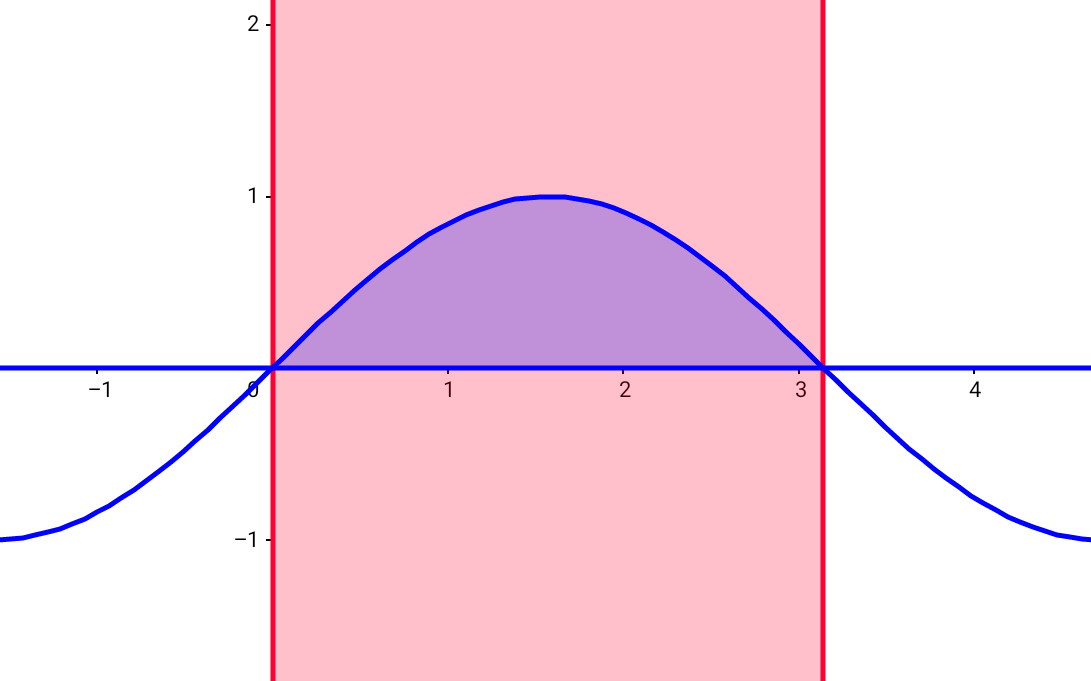
\includegraphics[width=0.5\textwidth, angle=0]{Grafico22.png}
\end{center}
\caption{}  
\end{figure}
\par
\vspace{1cm}
c) Primeiramente, observe a figura 18.
\begin{figure}[htbp]
\begin{center}
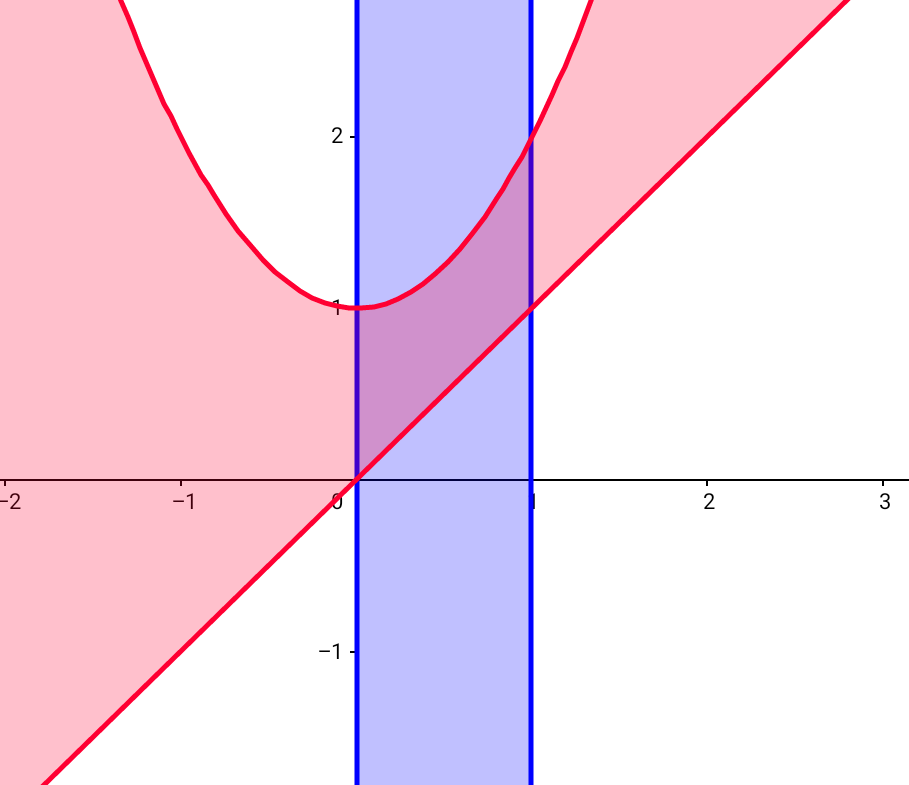
\includegraphics[width=0.5\textwidth, angle=0]{Grafico23.png}
\end{center}
\caption{}  
\end{figure}
\par Dela, segue que o volume desejado será:
\begin{equation*}\displaystyle{2\pi\cdot\int_{0}^{1}x(x^{2} + 1)\, dx - 2\pi\cdot\int_{0}^{1} x\cdot x\, dx = 2\pi\cdot\Big[ \Big(\frac{x^4}{4} + \frac{x^2}{2}\Big)\Big|^{1}_{0} - \Big(\frac{x^3}{3}\Big)\Big|^{1}_{0}    \Big] = \frac{5\pi }{6}.}\end{equation*}
\par
\vspace{0.3cm}
\subsection{Comprimento de gráfico de função}
\hspace{12pt}A seguir, vamos mostrar como obter o comprimento do gráfico de uma função num certo intervalo, dadas certas condições.
\par
\textbf{Demonstração.}
\par
Seja $y=f(x)$ com derivada contínua em $[a;b]$ e seja $P:a = x_0 < x_1 < x_2 < \cdots < x_{i-1} < x_i < \cdots < x_n = b$ uma partição de $[a;b]$. Indicando por $L(P)$ o comprimento da poligonal de vértices $P_{i} = (x_{i}, f(x_i)), i=1,2, ... , n$, temos:
$$\displaystyle{L(P) = \sum_{i=1}^{n}\sqrt{(x_i - x_{i-1})^2 + (f(x_i) - f(x_{i-1}))^2}.}$$
\par Geometricamente (pense no triângulo retângulo cuja hipotenusa é o comprimento aproximado da curva), podemos fazer $dx = x_i - x_{i-1}$ e $dy = f(x_i) - f(x_{i-1})$. Daí, segue que:
$$\displaystyle{L(P) = \sum_{i=1}^{n} \sqrt{(dx)^2 + (dy)^2} = \sum_{i=1}^{n} \sqrt{1 + \Big(\frac{dy}{dx}\Big)^2}\, dx .}$$
\par Calculando o limite para $n\rightarrow \infty $, temos que o comprimento $L$ de $y=f(x)$ em $[a;b]$ será:
$$\displaystyle{\lim_{n\to\infty }\sum_{i=1}^{n} \sqrt{1 + \Big(\frac{dy}{dx}\Big)^2}\, dx = \int_{a}^{b} \sqrt{1 + (f'(x))^2}\, dx .}$$\begin{flushright}$\blacksquare$ \end{flushright}
\par\textbf{Observação 1:} é possível provar essa fórmula usando o Teorema do Valor Médio, mas, como ele não foi apresentado aqui, essa prova não será mostrada.
\par\textbf{Observação 2:} note que calcular o comprimento de gráfico de função é, geralmente, mais difícil do que calcular o volume de um sólido de rotação.
\par
\vspace{0.3cm}
Exemplos.
\par
\begin{flushleft}
1. Calcule o comprimento do gráfico da função dada.
\end{flushleft}
\par
\begin{multicols}{3}
\hspace{-15pt}a) $\displaystyle{y = \frac{2}{3}x^{\frac{3}{2}}}$ , $\displaystyle{0\leq x\leq 1}$\\
b) $\displaystyle{y = e^{x}}$ , $\displaystyle{0\leq x\leq 1}$\\
c) $\displaystyle{y = \frac{e^x - e^{-x}}{2}}$ , $\displaystyle{0\leq x\leq 1}$
\end{multicols}
\vspace{0.3cm}
\par
\begin{flushleft}
1.1 Resolução.
\end{flushleft}
\par a) Como $y=\displaystyle{\frac{2}{3}x^{\frac{3}{2}}}$, $y' = \displaystyle{x^{\frac{1}{2}}}$. Logo, o comprimento $C$ de $y$ para $0\leq x\leq 1$ será:
\begin{equation*}\displaystyle{C = \int_{0}^{1} \sqrt{1 + x}\, dx = \frac{2}{3}\cdot (1+x)^{\frac{3}{2}}\Big|_{0}^{1} = \frac{2}{3} (2\sqrt{2} - 1).}\end{equation*}
\par
\vspace{0.3cm}
b) Note que $y' = e^{x}$. Portanto, o comprimento $C$ de $y$ para $0\leq x\leq 1$ é igual a:
\begin{equation*}\displaystyle{C = \int_{0}^{1} \sqrt{1 + e^{2x}}\, dx}.\end{equation*}
\par Tomando $u = \displaystyle{\sqrt{1 + e^{2x}}}$, segue:
\begin{equation*}\displaystyle{du = \frac{1}{2}2e^{2x}(1 + e^{2x})^{-\frac{1}{2}}\, dx \Rightarrow dx = \frac{u}{u^{2} - 1}\, du.}\end{equation*}
$$\displaystyle{\therefore C = \int_{\sqrt{2}}^{\sqrt{1 + e^{2}}} \frac{u^{2}}{u^{2} - 1}\, du = \int_{\sqrt{2}}^{\sqrt{1+e^{2}}}\, du + \int_{\sqrt{2}}^{\sqrt{1+e^{2}}} \frac{1}{u^{2} - 1}\, du.}$$
\par Utilizando frações parciais para a segunda integral, temos:
$$\displaystyle{C = \sqrt{1 + e^{2}} - \sqrt{2} + \frac{1}{2}\cdot\Big(\ln{\Big|\frac{u-1}{u+1}\Big|}\Big)\Big|_{\sqrt{2}}^{\sqrt{1+e^{2}}} = 1 + \sqrt{1 + e^{2}} - \sqrt{2} + \ln{\Big(\frac{1 + \sqrt{2}}{1 + \sqrt{1+e^{2}}}\Big)} .}$$        
\par
\vspace{0.3cm}
c) Note que $y' = \displaystyle{\frac{e^x - e^{-x}}{2}}$. Daí, segue que o comprimento $C$ de $y$ para $1\leq x\leq 0$ será:
\begin{equation*}\displaystyle{C = \int_{0}^{1} \sqrt{1 + \frac{e^{2x} - 2 + e^{-2x}}{4}} dx = \frac{1}{2}\int_{0}^{1} \sqrt{e^{2x} + 2 + e^{-2x}}\, dx = \frac{1}{2}\int_{0}^{1} e^x + e^{-x}\, dx = \frac{1}{2} (e^{x} - e^{-x})\Big|_{0}^{1} = \frac{1}{2}(e - e^{-1}).}\end{equation*}
\par
\vspace{0.3cm}
\subsection{Exercícios - Integral}
\par
\begin{flushleft}
1. Calcule $\displaystyle{\int \sec^{3}{x}\, dx}$.
\end{flushleft}
\par
\vspace{0.3cm}
\begin{flushleft}
1.1 Resolução.
\end{flushleft}
\par Note que $\displaystyle{\int \sec^{3}{x}\, dx = \int \sec^{2}{x}\cdot\sec{x}\, dx}$.
\par Fazendo $u = \sec{x}$ e $dv = \sec^{2}{x}\, dx$, segue:
\begin{equation*}\displaystyle{du = \sec{x}\tan{x}\, dx , v = \tan{x} .}\end{equation*}
\par Daí, vem:
\begin{equation*}\displaystyle{\begin{split}
\therefore\int\sec^{3}{x}\, dx &=\sec{x}\tan{x}-\int\tan^{2}{x}\sec{x}\, dx= \\ &=\sec{x}\tan{x}-\int (\sec^{3}{x}-\sec{x})\, dx= \\
&=\sec{x}\tan{x}-\int\sec^{3}{x}\, dx+\int\sec{x}\, dx
\therefore 2\cdot\int\sec^{3}{x}\, dx=\sec{x}\tan{x}+\int\sec{x}\, dx \\ \Rightarrow\int\sec^{3}{x}\, dx &=\frac{1}{2}\cdot\sec{x}\cdot\tan{x}+ \frac{1}{2}\cdot\ln{|\sec{x}+\tan{x}|}+c, c\in\mathbb{R}.
\end{split}}\end{equation*}
\par
\vspace{0.3cm}
\begin{flushleft}
2. Calcule, utilizando uma integral definida, a área do conjunto de todos os pontos $(x,y)\in\mathbb{R}^2$ tais que $\displaystyle{\frac{x^{2}}{a^{2}} + \frac{y^{2}}{b^{2}} \leq 1}$, com $a > 0$ e $b > 0$ fixos. 
\end{flushleft}
\par
\vspace{0.3cm}
\begin{flushleft}
2.1 Resolução.
\end{flushleft}
\par Suponha, sem perda de generalidade, que $y > 0$. A inequação $\displaystyle{\frac{x^{2}}{a^{2}} + \frac{y^{2}}{b^{2}} \leq 1}$ nos dá a região interna de uma elipse de equação $\displaystyle{\frac{x^2}{a^2} + \frac{y^2}{b^2} = 1}$. Isolando $y$, temos:
\begin{equation*}\displaystyle{\frac{y^2}{b^2} = 1 - \frac{x^2}{a^2} \Rightarrow y = \frac{b}{a}\sqrt{a^{2} - x^{2}} .}\end{equation*}
\par Logo, decorre da simetria que a área da elipse é dada por:
\begin{equation*}\displaystyle{2\cdot\int_{-a}^{a}\frac{b}{a}\sqrt{a^2 - x^2}\, dx = \frac{2b}{a}\cdot\int_{-a}^{a} \sqrt{a^2 - x^2}\, dx .}\end{equation*}
\par Note que $\displaystyle{\sqrt{a^2 - x^2}}$ pode ser visto como o segundo cateto de um triângulo retângulo de hipotenusa $a$ e cateto $x$. Chamando de $\theta $ o ângulo relativo a $x$, temos:
\begin{equation*}\displaystyle{\sin{\theta } = \frac{x}{a} \Rightarrow x = a\sin{\theta } \Rightarrow dx = a\cos{\theta }\, d\theta .}\end{equation*}
$$\displaystyle{\begin{split}\therefore \frac{2b}{a}\cdot\int_{-a}^{a} \sqrt{a^2 - x^2}\, dx &= \frac{2b}{a}\cdot\int_{-\frac{\pi }{2}}^{\frac{\pi }{2}} \sqrt{a^2 - a^{2}\sin^{2}{\theta }} \cdot a\cos{\theta } \, d\theta = \\ &= \frac{2b}{a}\cdot\int_{-\frac{\pi }{2}}^{\frac{\pi }{2}} a^{2}\sqrt{\cos^{2}{\theta }} \cdot\cos{\theta }\, d\theta = \\ &= 2ab\cdot\int_{-\frac{\pi }{2}}^{\frac{\pi }{2}} \cos^{2}{\theta }\, d\theta = \\ &= 2ab\cdot\int_{-\frac{\pi }{2}}^{\frac{\pi }{2}} \Big(\frac{1}{2} + \frac{1}{2}\cos{2\theta }\Big)\,  d\theta = \\ &= ab\cdot\Big(\theta + \frac{\sin{2\theta }}{2}\Big)\Big|_{-\frac{\pi }{2}}^{\frac{\pi }{2}} = \\ &= \pi ab .\end{split}}$$
\par
\vspace{0.3cm}
\begin{flushleft}
3. Calcule, utilizando uma integral definida, o volume de uma calota esférica de raio $r$ e altura $h$.
\end{flushleft}
\par
Seja $R$ o raio da esfera. Note que podemos obter tal esfera rotacionando, em torno do eixo $x$, a região definida pelos pontos $(x,y)\in\mathbb{R}^2$ tais que $\displaystyle{0\leq y \leq\sqrt{R^{2} - x^{2}}}$ e $\displaystyle{-R\leq x\leq R}$. Similarmente, a calota esférica pode ser obtida rotacionando-se a região, em torno do eixo $x$, definida pelos pontos $(x,y)\in\mathbb{R}^2$ tais que $\displaystyle{0\leq y\leq\sqrt{R^{2} - x^{2}}}$ e $\displaystyle{R-h \leq x \leq R}$. Daí, segue que o volume da calota será dado por:
\begin{equation*}\displaystyle{\pi\cdot\int_{R-h}^{R} y^{2}\, dx = \pi\cdot\int_{R-h}^{R} (R^{2} - x^{2})\, dx = \pi\cdot\Big(xR^{2} - \frac{x^3}{3}\Big)\Big|_{R-h}^{R} = \frac{\pi h^{2}}{3}(3R - h).}\end{equation*}

\end{newpage}}\end{document}